%%!TEX root = ./marylie.tex
%%--.----1----.----2----.----3----.----4----.----5----.----6----.----7----.-!

\chapter{Simple Examples of Use of MaryLie}

\section{Overview}
     Subsequent  chapters of this manual are devoted to an exposition of the theory and application of \Maryend.  The purpose of this chapter is to
intrigue the reader with a few simple, sometimes whimsical, examples of the
use of \Maryend.  At this stage, the reader may read as much or as little of
these examples as desired.  It is suggested that the reader look at the
first example, and then at any other examples of interest.  For
convenience, the examples and their section numbers are listed below.
Further examples are given in Chapter 10.  It
will be seen that \Mary is essentially a {\em programming language}
that enables the user to simulate, analyze, and manipulate a vast variety
of both beamlines and circular machines.

\contentsline {section}{\numberline {2.2}Simple Spot Forming System}{\pageref{simplespot}}
\contentsline {section}{\numberline {2.3}Simple Imaging System}{\pageref{simpleimage}}
\contentsline {section}{\numberline {2.4}Simple Spectrometer}{\pageref{simplespec}}
\contentsline {section}{\numberline {2.5}Small Static Storage Ring}{\pageref{staticstorage}}
\contentsline {section}{\numberline {2.6}Small Storage Ring with Bunchers}{\pageref{ringbunchers}}
\contentsline {section}{\numberline {2.7}Large Storage Ring}{\pageref{largering}}

     The first three examples are of single pass systems, and the remaining
examples are of circulating storage systems.  Each of these examples could
be a research project in its own right.  In general, this research has not
been done.  Consequently, the parameter values employed may not be optimal,
and are not necessarily even of physical interest.

The \Mary 3.0 input and output for these examples will be given in detail,
and may be of interest to the reader for later reference.  However, only
the highlights of the calculations will be described.  After the reader
has read the remainder of the manual, she or he should be able to
understand the examples in detail.

\section{Simple Spot Forming System}
\label{simplespot}
     Consider the simple spot forming system\index{spot forming system} shown in figure 2.2.1 below.
It consists of a quadrupole triplet followed by a drift space.\index{triplet}  The
quadrupole strengths and the drift lengths have been selected in such a way
that (in linear paraxial approximation) incoming parallel rays are brought
to a final point focus.  Such a system could be the basis of a microprobe.\index{microprobe}


\begin{figure}[htbp]
  \centering
  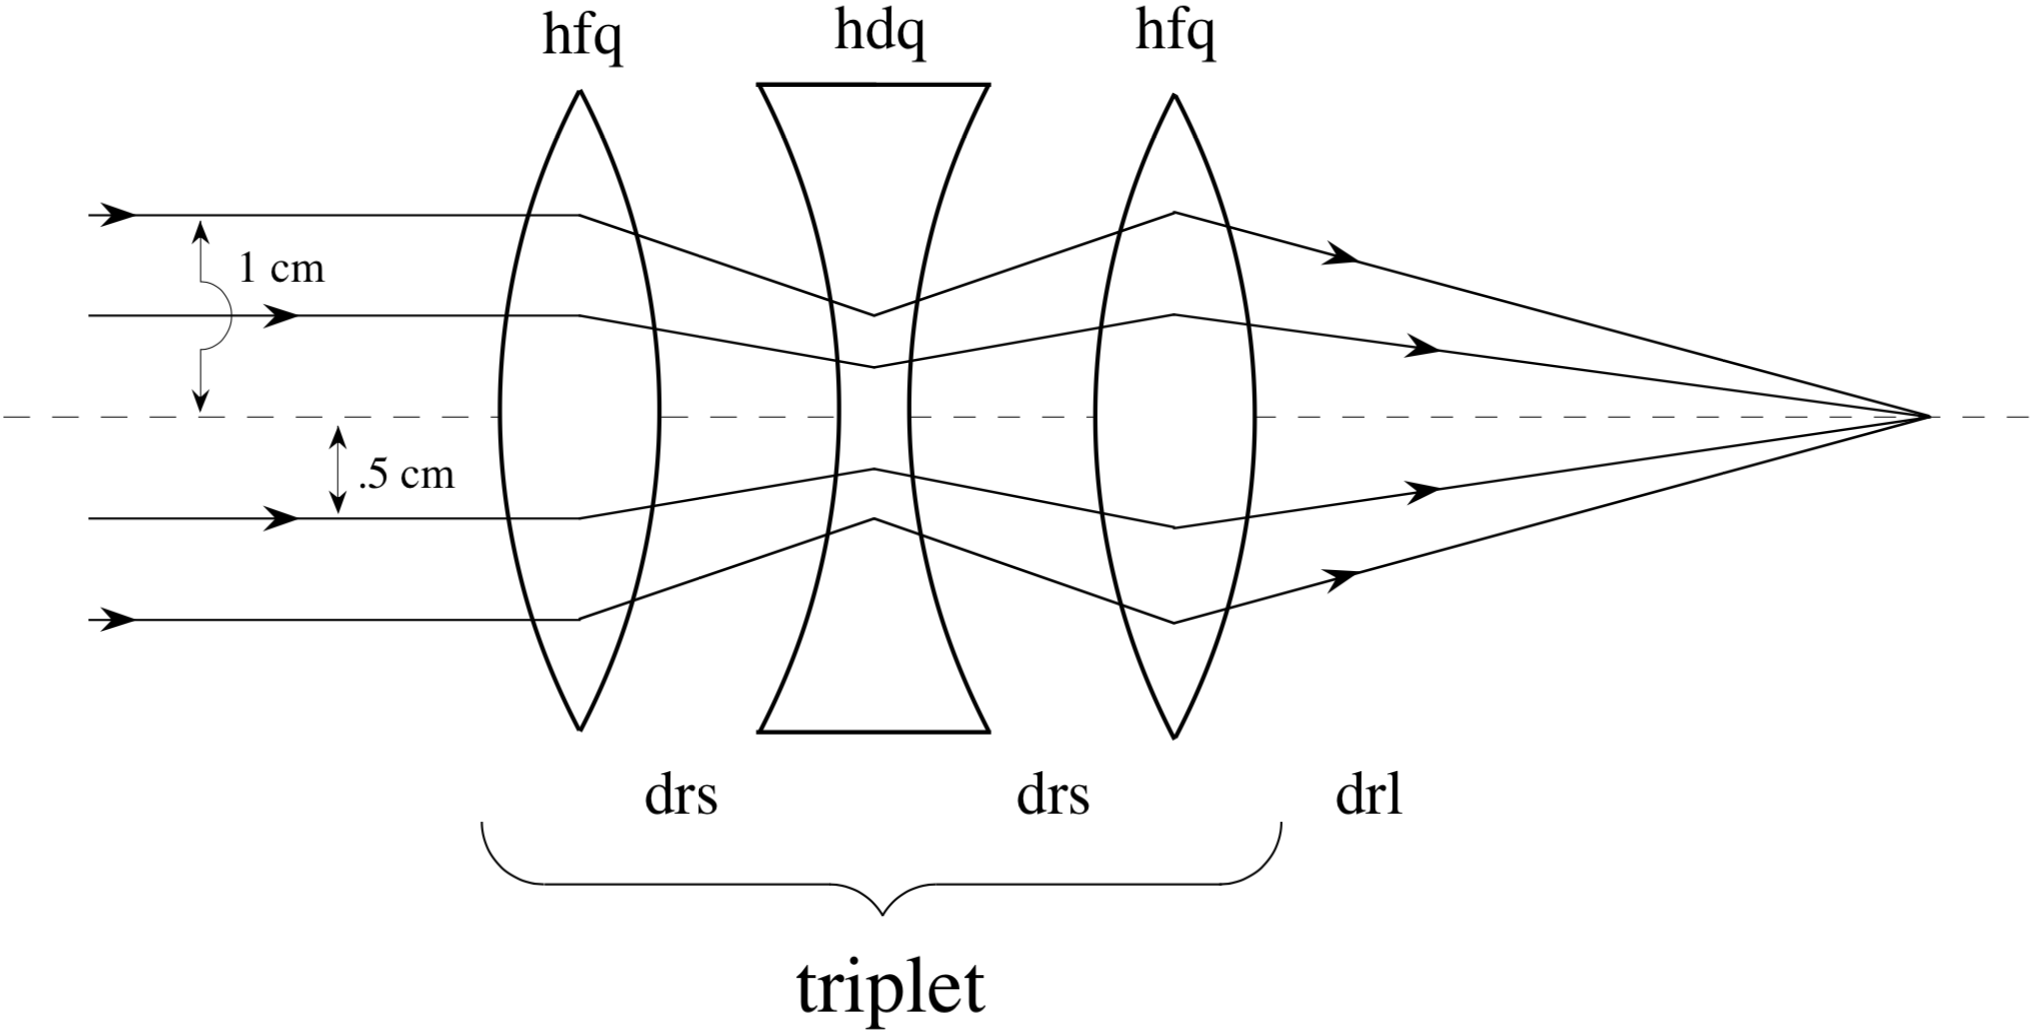
\includegraphics[scale=0.453]{Triplet}
  \caption{Schematic of Simple Spot Forming System.}
\end{figure}

\pagebreak

   How well does this system work when account is taken of nonlinear
effects? Shown below is the Master Input File for a \Mary 3.0 run set up
to trace rays through this system.

{\footnotesize\tt
\begin{verbatim}
 #comment
  Exhibit 2.2.1.
  This is a study of a simple spot forming system.
 #beam
   1.035274408519500
  5.3289019605700000E-02
   1.000000000000000
   1.000000000000000
 #menu
  drs      drft
   0.500000000000000
  drl      drft
    20.0026000000000
  hfq      quad
    1.50000000000000      8.630000000000000E-02   1.00000000000000
    1.00000000000000
  hdq      quad
    3.00000000000000     -8.289450000000000E-02   1.00000000000000
    1.00000000000000
  fileout  pmif
    1.00000000000000       12.0000000000000       3.00000000000000
  mapout   ptm
    3.00000000000000       3.00000000000000      0.000000000000000E+00
   0.000000000000000E+00   1.00000000000000
  rays     rt
    13.0000000000000       14.0000000000000       5.00000000000000
    1.00000000000000       1.00000000000000      0.000000000000000E+00
  end      end
 #lines
  trip
      1*hfq         1*drs         1*hdq         1*drs         1*hfq
  spot
      1*trip        1*drl
 #lumps
 #loops
 #labor
     1*fileout
     1*spot
     1*rays
     1*end
\end{verbatim}}

     The reader will observe that the Master Input File\index{master input file} is organized into
seven components.  They are {\em \#comments}, {\em \#beam}, {\em \#menu}, {\em \#lines}, {\em \#lumps},
{\em \#loops}, and {\em \#labor}, respectively.  The {\em \#comments} component allows the user
to write comments about the system under study, the calculations to be
performed, etc. The {\em \#beam} component specifies the design magnetic rigidity
(in Tesla-meters) and the corresponding relativistic $\beta$ and $\gamma$ factors for
the beam to be ``transported'' by the system.  It also specifies $|q/e|$,
the absolute charge in units of $e$, and the scale
length to be employed for the spatial components of phase-space
variables.  See Section 5.6.3.
For this example, the incoming beam is taken to consist of 50 MeV protons,
and the scale length is taken to be 1 meter.

The {\em \#menu} component is a list of user specified beamline elements and
commands.  Each item on the menu consists of a user specified name followed
by a \Mary type code mnemonic.  The numbers following each menu item
specify lengths, strengths, and other required parameters.  For example,
{\em drs } is a short drift of length .5 meters.  Similarly, {\em hfq }is a horizontally
focusing quadrupole of length 1.5 meters and strength .0863 Tesla/meter.
The two remaining parameters for this quadrupole (both set equal to +1 in
this example) indicate that it is to be treated as having hard-edge leading
and trailing fringe fields.  Finally, {\em fileout}, {\em mapout}, {\em rays}, and {\em end }are four commands.

The {\em \#lines} component contains a list of user specified names for
collections of elements and/or commands drawn from the menu.  In this case,
{\em trip } refers to the quadrupole triplet system, and {\em spot } refers to the entire
spot forming system.  See figure 2.2.1.

     In this simple example, the {\em \#lumps} and {\em \#loops} components are empty,
and are not used.  Their function will be described in later examples.

Finally, the {\em \#labor} component specifies the system to be considered, and
the actual operations and calculations to be performed.  In this case,
{\em fileout } causes the Master Input File to be printed out; {\em spot } causes the
calculation of the transfer map for the entire system; {\em rays } produces a
trace of rays through the system; and {\em end } signifies the end of the
calculation.  Note that so far, in this example, the command {\em mapout } is not
actually used since it neither appears nor is referenced in {\em \#labor}.

When \Mary 3.0 is run using the Master Input File just described,
the following output is produced:

{
\footnotesize\tt
\begin{verbatim}
 #comment
  Exhibit 2.2.2.
  This is a study of a simple spot forming system.
 #beam
   1.035274408519500
  5.3289019605700000E-02
   1.000000000000000
   1.000000000000000
 #menu
  drs      drft
   0.500000000000000
  drl      drft
    20.0026000000000
  hfq      quad
    1.50000000000000      8.630000000000000E-02   1.00000000000000
    1.00000000000000
  hdq      quad
    3.00000000000000     -8.289450000000000E-02   1.00000000000000
    1.00000000000000
  fileout  pmif
    1.00000000000000       12.0000000000000       3.00000000000000
  mapout   ptm
    3.00000000000000       3.00000000000000      0.000000000000000E+00
   0.000000000000000E+00   1.00000000000000
  rays     rt
    13.0000000000000       14.0000000000000       5.00000000000000
    1.00000000000000       1.00000000000000      0.000000000000000E+00
  time     time
   1.00000000000000       12.0000000000000       3.00000000000000
  end      end

 #lines
  trip
      1*hfq         1*drs         1*hdq         1*drs         1*hfq
  spot
      1*trip        1*drl
 #lumps
 #loops
 #labor
     1*fileout
     1*spot
     1*rays
     1*time
     1*end

  execution time in seconds =   6.48
\end{verbatim}}
\noindent Note that the Master Input File is printed as a result of the presence of
the command {\em fileout } in {\em \#labor}.  However, relatively little else is printed.

    The major task of this run is to trace rays.  This is accomplished by
the presence of the {\em rays } command in {\em \#labor}.  When this command is
encountered, initial conditions are read in from a previously prepared
external file.  The total transfer map for the system is then applied to
each initial condition, and the results are written on another external
file.  The first few lines of each of these files are shown below:
\vspace{5mm}
\pagebreak

First few lines of initial condition file for ray traces
\begin{footnotesize}
\begin{tt}
\begin{tabbing}
0.100\=0E-01 0.000\=0E+00 0.000\=0E+00 0.000\=0E+00 0.000\=0E+00 0.000\=0E+00 \kill
\>$X$ \>$P_x$ \>$Y$ \>$P_y$ \>$\tau$ \>$P_{\tau}$
\end{tabbing}
\end{tt}
\vspace{-5mm}
\begin{verbatim}
0.1000E-01 0.0000E+00 0.0000E+00 0.0000E+00 0.0000E+00 0.0000E+00
0.9980E-02 0.0000E+00 0.6279E-03 0.0000E+00 0.0000E+00 0.0000E+00
0.9921E-02 0.0000E+00 0.1253E-02 0.0000E+00 0.0000E+00 0.0000E+00
0.9823E-02 0.0000E+00 0.1874E-02 0.0000E+00 0.0000E+00 0.0000E+00
\end{verbatim}
\end{footnotesize}
\vspace{5mm}

First few lines of final condition file resulting from ray traces
\begin{footnotesize}
\begin{tt}
\begin{tabbing}
-1.699\=89E-07 -4.012\=00E-04 -9.380\=35E-08 -5.491\=85E-05 9.898\=83E-06 0.000\= \kill
\>$X$ \>$P_x$ \>$Y$ \>$P_y$ \>$\tau$ \>$P_{\tau}$
\end{tabbing}
\end{tt}
\vspace{-5mm}
\begin{verbatim}
-1.61053E-07 -4.04394E-04  0.00000E+00  0.00000E+00 9.78473E-06 0.00000E+00
-1.63302E-07 -4.03585E-04 -4.72204E-08 -2.75206E-05 9.81295E-06 0.00000E+00
-1.69989E-07 -4.01200E-04 -9.38035E-08 -5.49185E-05 9.89883E-06 0.00000E+00
 1.80829E-07 -3.97237E-04 -1.39245E-07 -8.21367E-05 1.00411E-05 0.00000E+00
\end{verbatim}
\end{footnotesize}

There are six numbers in each line corresponding to the coordinates in
6-dimensional phase space.  The first four coordinates describe the
transverse phase space.  The last two describe the differential time of
flight $\tau$ and its conjugate momentum $P_\tau$  (which, as will be described later,
is related to energy deviation).

As indicated in figure 2.2.1, the incoming rays are selected
to be {\em parallel} to the optical axis and to lie on two cylinders having radii of
1.0 cm and 0.5 cm respectively.  Consequently, the $P_x$  and $P_y$  entries in
the initial condition file (those entries which describe transverse momenta)
are all zero.  Figure 2.2.2 below shows the result of plotting the first and
third columns (the X and Y phase space coordinates) of the initial
condition file. Altogether, 200 rays are shown.  As advertized, the
incoming rays do indeed lie on two cylinders.

\begin{figure}[hbp]
  \centering
  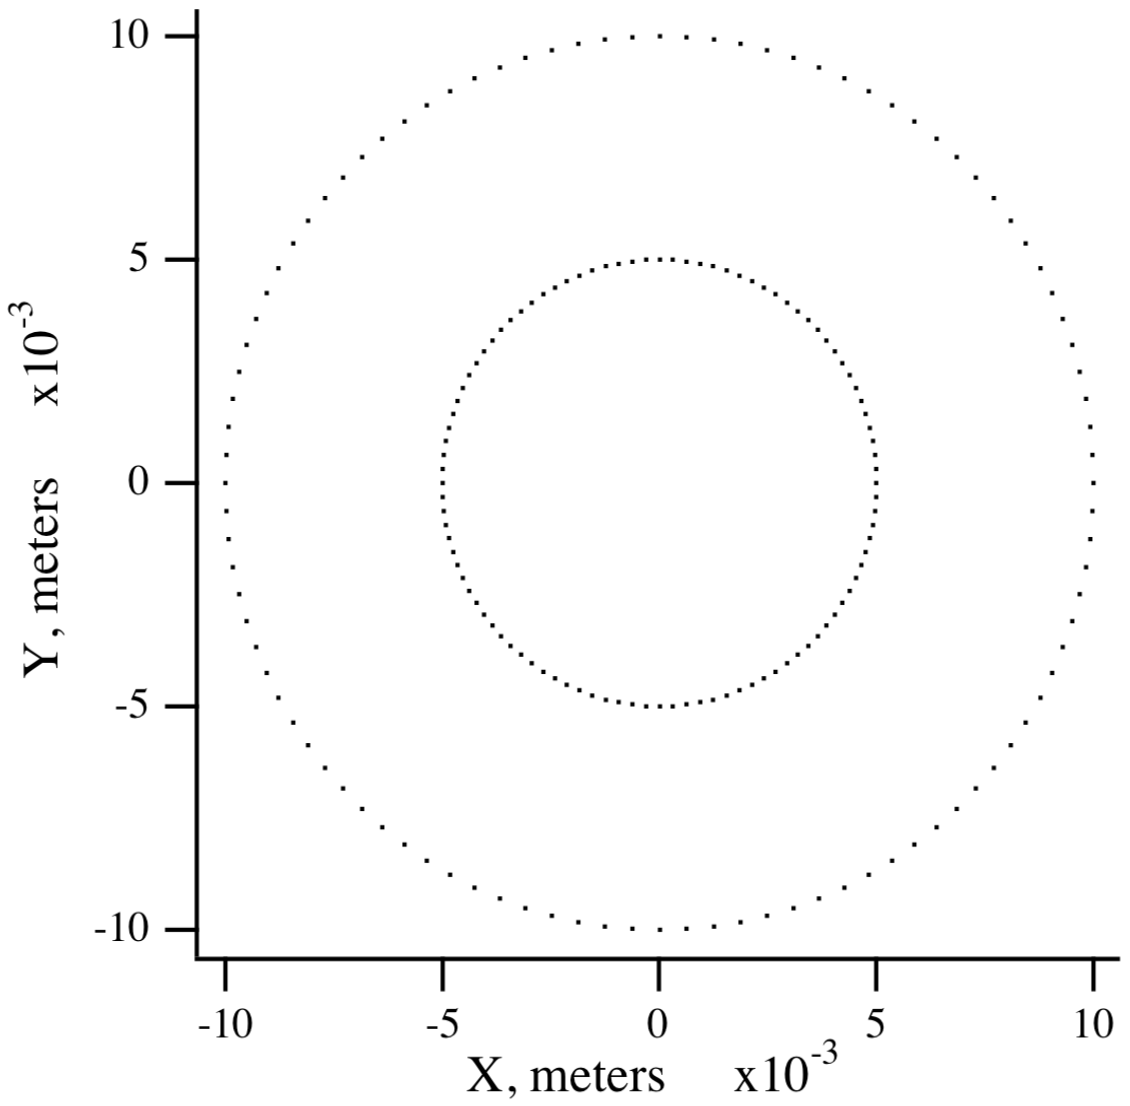
\includegraphics[height=3.5in]{spot}
  \caption{Plot of Initial Conditions for Incoming Rays of Spot Forming System.}
\end{figure}

     If the performance of the spot forming system were perfect, the X and
Y entries in the final condition file (resulting from the ray trace) would
all be zero.  Inspection of the first few lines of the final condition file
shows that the X and Y entries are indeed small.  However, they are not
zero.  In fact, their finite value is due to the presence of third-order
``spherical type'' aberrations.  These aberrations come primarily from
nonlinear effects associated with quadrupole fringe fields.

Figure 2.2.3 displays the result of plotting the X and Y entries of the
final condition file.  It shows that the incoming cylinders of parallel
rays are not focused to a single point spot.  Rather, they produce two
``hour glass'' shaped figures.  The inner and outer hour glasses come from
the inner and outer cylinders respectively.

     Examination of the figure shows that the relative sizes of the two
hour glasses is about 8 to 1.  By contrast, the ratio of the two cylinder
sizes in figure 2.2.2 is 2 to 1.  This is just what is to be expected from
third-order aberration effects since $2^3=8$.

\begin{figure}[hbp]
  \centering
  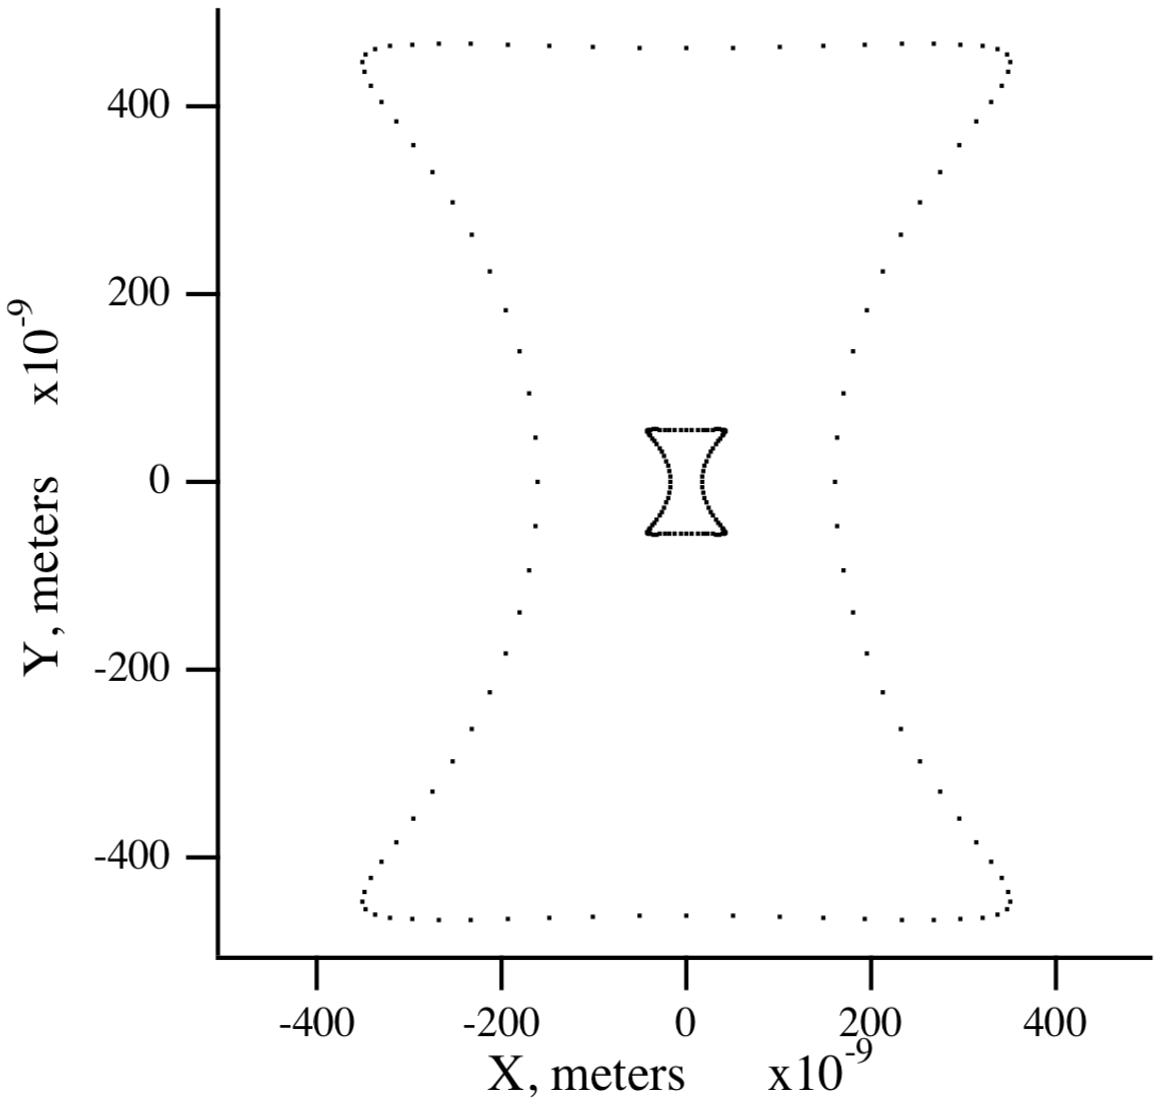
\includegraphics[height=3.5in]{spotfin}
  \caption{Focal spot pattern produced by two incoming cylinders of parallel rays.}
\end{figure}

     The relative importance of the various aberrations (through third
order) can be examined in quantitative detail by printing out the Lie
algebraic representation of the total transfer map for the spot forming
system.  This can be accomplished by including the command {\em mapout} in
{\em \#labor}.  Shown below is the result of such a \Mary 3.0 run.
\pagebreak

{
\footnotesize\tt
\begin{verbatim}
 #comment
  Exhibit 2.2.3.
  This is a study of a simple spot forming system.
 #beam
   1.035274408519500
  5.3289019605700000E-02
   1.000000000000000
   1.000000000000000
 #menu
  drs      drft
   0.500000000000000
  drl      drft
    20.0026000000000
  hfq      quad
    1.50000000000000      8.630000000000000E-02   1.00000000000000
    1.00000000000000
  hdq      quad
    3.00000000000000     -8.289450000000000E-02   1.00000000000000
    1.00000000000000
  fileout  pmif
    1.00000000000000       12.0000000000000       3.00000000000000
  mapout   ptm
    3.00000000000000       3.00000000000000      0.000000000000000E+00
   0.000000000000000E+00   1.00000000000000
  rays     rt
    13.0000000000000       14.0000000000000       5.00000000000000
    1.00000000000000       1.00000000000000      0.000000000000000E+00
  end      end
 #lines
  trip
      1*hfq         1*drs         1*hdq         1*drs         1*hfq
  spot
      1*trip        1*drl
 #lumps
 #loops
 #labor
     1*fileout
     1*spot
     1*mapout
     1*end

 matrix for map is :

 7.43444E-07  2.47288E+01  0.00000E+00  0.00000E+00 0.00000E+00 0.00000E+00
-4.04387E-02  8.08880E-01  0.00000E+00  0.00000E+00 0.00000E+00 0.00000E+00
 0.00000E+00  0.00000E+00  7.22568E-07  2.28173E+01 0.00000E+00 0.00000E+00
 0.00000E+00  0.00000E+00 -4.38264E-02  8.76642E-01 0.00000E+00 0.00000E+00
 0.00000E+00  0.00000E+00  0.00000E+00  0.00000E+00 1.00000E+00 2.46784E+02
 0.00000E+00  0.00000E+00  0.00000E+00  0.00000E+00 0.00000E+00 1.00000E+00

 nonzero elements in generating polynomial are :

  f( 33)=f( 20 00 01 )=-0.45766053436970D-01
  f( 38)=f( 11 00 01 )= 0.14345982412058D+01
  f( 53)=f( 02 00 01 )=-0.59832851277335D+02
  f( 67)=f( 00 20 01 )=-0.10955092926799D+00
  f( 70)=f( 00 11 01 )= 0.46810944831432D+01
  f( 76)=f( 00 02 01 )=-0.88881809079482D+02
  f( 83)=f( 00 00 03 )=-0.39290849771004D+03
  f( 84)=f( 40 00 00 )=-0.16965902443077D-02
  f( 85)=f( 31 00 00 )= 0.16215419632088D+00
  f( 90)=f( 22 00 00 )=-0.59484282516103D+01
  f( 95)=f( 20 20 00 )=-0.16646388617124D-01
  f( 96)=f( 20 11 00 )= 0.75198181482571D+00
  f( 99)=f( 20 02 00 )=-0.85538134290315D+01
  f(104)=f( 20 00 02 )=-0.19073142049137D+00
  f(105)=f( 13 00 00 )= 0.99159110467675D+02
  f(110)=f( 11 20 00 )= 0.80660002769129D+00
  f(111)=f( 11 11 00 )=-0.36679597123554D+02
  f(114)=f( 11 02 00 )= 0.41993959894126D+03
  f(119)=f( 11 00 02 )= 0.78836842993921D+01
  f(140)=f( 04 00 00 )=-0.63693341340996D+03
  f(145)=f( 02 20 00 )=-0.10046981396547D+02
  f(146)=f( 02 11 00 )= 0.45984530773432D+03
  f(149)=f( 02 02 00 )=-0.53047221347237D+04
  f(154)=f( 02 00 02 )=-0.30942962923253D+03
  f(175)=f( 00 40 00 )=-0.51353235082385D-02
  f(176)=f( 00 31 00 )= 0.46634415070127D+00
  f(179)=f( 00 22 00 )=-0.15935461945328D+02
  f(184)=f( 00 20 02 )=-0.58685382925631D+00
  f(185)=f( 00 13 00 )= 0.24279242171843D+03
  f(190)=f( 00 11 02 )= 0.32524382342626D+02
  f(195)=f( 00 04 00 )=-0.13944546806254D+04
  f(200)=f( 00 02 02 )=-0.60171761738398D+03
  f(209)=f( 00 00 04 )=-0.15330379170756D+04
\end{verbatim}}

     Again, the Master Input File is printed because the command {\em fileout } is
still in {\em \#labor}.  In addition, the transfer matrix is printed as a result
of the command {\em mapout } in {\em \#labor}.  Note that the 1,1 and 3,3 entries for the
transfer matrix are very small.  (Indeed, they could be made to vanish
exactly by slightly adjusting various parameter values.)  That, of course,
is what is required of a spot forming system.

Finally, again as a result of the command {\em mapout}, the nonzero elements
in the Lie algebraic generating polynomial are printed.  As will be
described later, this polynomial characterizes the nonlinear parts of the
transfer map. In particular, ``spherical type'' aberrations are controlled by
the coefficients numbered 140, 149, and 195.  Inspection shows that these
coefficients are quite large in this example.

\section{Simple Imaging System}
\label{simpleimage}
     Consider the problem of analyzing the performance of a simple imaging
system\index{imaging system}, half of which is shown in figure 2.3.1 below.  The system is
required to provide unit magnification when acting on rays of 20 TeV
protons, and is made with superconducting magnets.  It consists of four
quadrupole doublets, and various drifts.\index{doublet}
\pagebreak


\begin{figure}[htb]
  \centering
  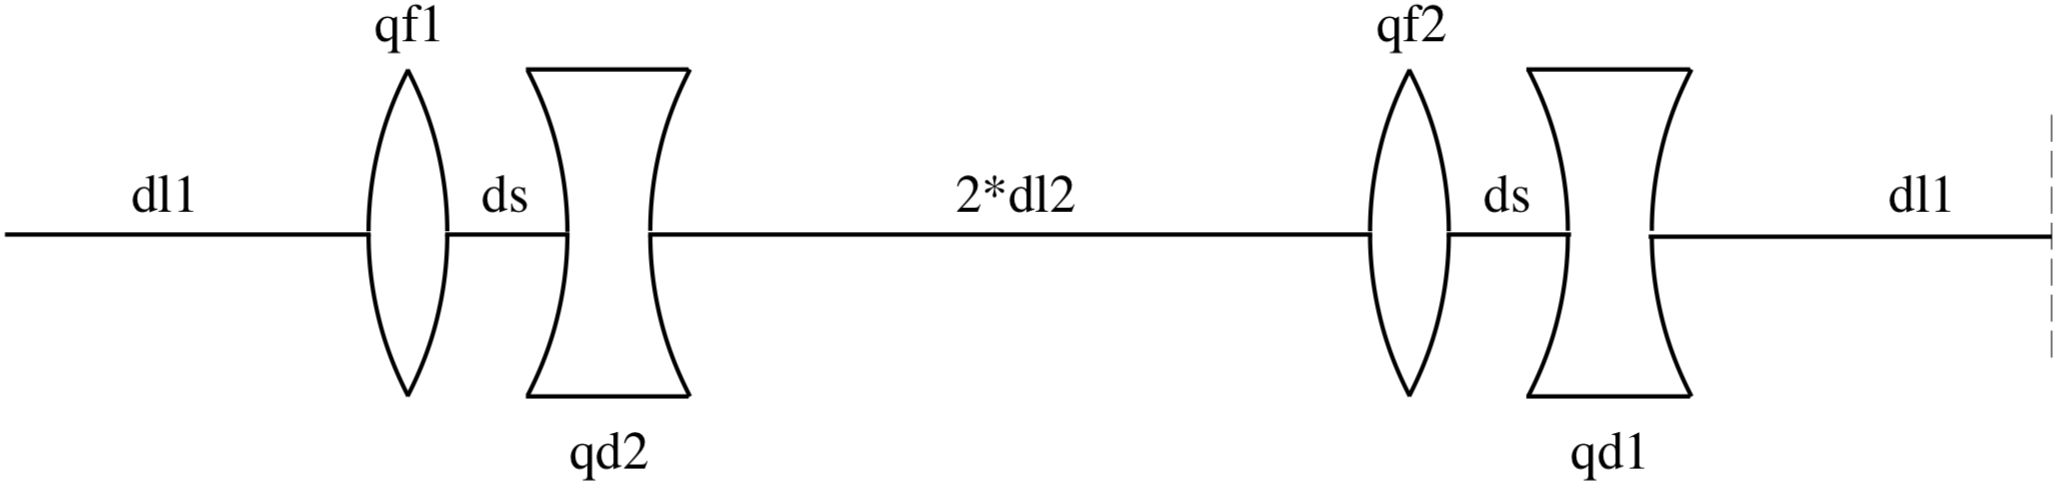
\includegraphics[scale=0.453]{HalfCell}
  \caption{Half Cell of Simple Quadrupole Imaging System.}
\end{figure}

The result of a \Mary 3.0 run, structured to compute the transfer
map for this system and then trace rays, is shown below:

{
\footnotesize\tt
\begin{verbatim}
 #comment
  Exhibit 2.3.1.
  This is a study of a simple imaging system.
 #beam
   66710.00000000000
   21315.00000000000
   1.000000000000000
   1.000000000000000
 #menu
  dl1      drft
    99.9898870000000
  dl2      drft
    100.000000000000
  ds       drft
    5.00000000000000
  qf1      quad
    10.0000000000000       192.642380000000       1.00000000000000
    1.00000000000000
  qf2      quad
    10.0000000000000       192.642395000000       1.00000000000000
    1.00000000000000
  qd1      quad
    10.0000000000000      -192.642380000000       1.00000000000000
    1.00000000000000
  qd2      quad
    10.0000000000000      -192.642395000000       1.00000000000000
    1.00000000000000
  end      end
  rays     rt
    13.0000000000000       14.0000000000000       5.00000000000000
    1.00000000000000       1.00000000000000      0.000000000000000E+00
  mapout   ptm
    3.00000000000000       3.00000000000000      0.000000000000000E+00
   0.000000000000000E+00   1.00000000000000
  fileout  pmif
    1.00000000000000       12.0000000000000       3.00000000000000
 #lines
  half
      1*dl1         1*qf1         1*ds          1*qd2         2*dl2
&
      1*qf2         1*ds          1*qd1         1*dl1
  image
      2*half
 #lumps
 #loops
 #labor
     1*fileout
     1*image
     1*mapout
     1*end


 matrix for map is :

 9.99856E-01 -1.28018E-06  0.00000E+00  0.00000E+00 0.00000E+00 0.00000E+00
-3.22156E-06  1.00014E+00  0.00000E+00  0.00000E+00 0.00000E+00 0.00000E+00
 0.00000E+00  0.00000E+00  1.00014E+00 -1.28018E-06 0.00000E+00 0.00000E+00
 0.00000E+00  0.00000E+00 -3.22156E-06  9.99856E-01 0.00000E+00 0.00000E+00
 0.00000E+00  0.00000E+00  0.00000E+00  0.00000E+00 1.00000E+00 1.98067E-06
 0.00000E+00  0.00000E+00  0.00000E+00  0.00000E+00 0.00000E+00 1.00000E+00
 nonzero elements in generating polynomial are :

  f( 33)=f( 20 00 01 )=-0.38872686692784D-01
  f( 38)=f( 11 00 01 )= 0.34566885965630D+01
  f( 53)=f( 02 00 01 )=-0.48798663436745D+03
  f( 67)=f( 00 20 01 )=-0.38872615870228D-01
  f( 70)=f( 00 11 01 )=-0.34598333034969D+01
  f( 76)=f( 00 02 01 )=-0.48812740619185D+03
  f( 83)=f( 00 00 03 )=-0.99033373115764D-06
  f( 84)=f( 40 00 00 )=-0.83288898279040D-04
  f( 85)=f( 31 00 00 )= 0.25161405938893D-01
  f( 90)=f( 22 00 00 )=-0.62836326304276D+01
  f( 95)=f( 20 20 00 )=-0.30874907661279D-03
  f( 96)=f( 20 11 00 )= 0.23903124877554D-03
  f( 99)=f( 20 02 00 )=-0.39026732544282D+01
  f(104)=f( 20 00 02 )=-0.97111094673821D-01
  f(105)=f( 13 00 00 )= 0.32933448063609D+03
  f(110)=f( 11 20 00 )=-0.31327507049347D-03
  f(111)=f( 11 11 00 )=-0.15267268376928D+02
  f(114)=f( 11 02 00 )= 0.17231939107284D+02
  f(119)=f( 11 00 02 )= 0.86317322338312D+01
  f(140)=f( 04 00 00 )=-0.13424150978119D+05
  f(145)=f( 02 20 00 )=-0.39004786583392D+01
  f(146)=f( 02 11 00 )=-0.17546489785270D+02
  f(149)=f( 02 02 00 )=-0.49593499786268D+05
  f(154)=f( 02 00 02 )=-0.39715437881394D+03
  f(175)=f( 00 40 00 )=-0.83321956145577D-04
  f(176)=f( 00 31 00 )=-0.25194640841094D-01
  f(179)=f( 00 22 00 )=-0.62868169322496D+01
  f(184)=f( 00 20 02 )=-0.97110897267768D-01
  f(185)=f( 00 13 00 )=-0.32960255997846D+03
  f(190)=f( 00 11 02 )=-0.86342917628377D+01
  f(195)=f( 00 04 00 )=-0.13431897330774D+05
  f(200)=f( 00 02 02 )=-0.39726895527551D+03
  f(209)=f( 00 00 04 )=-0.99033373279231D-06
\end{verbatim}}

     The {\em \#lines} component of the Master Input File defines the entire
optical system in terms of the line called {\em image}.  The contents of the line
{\em image } is in turn defined in terms of the line {\em half}.  The contents of the
line {\em half } is the same as that shown in figure 2.3.1.

     The key entries in the {\em \#labor} component of the Master Input File are {\em image}, {\em mapout}, and {\em rays}.  The entry {\em image } calls for the computation of the transfer map described by the line {\em image}.  The commands {\em mapout } and {\em rays } then call for the printing of the map and the tracing of rays through the system

   Inspection of the transfer matrix for the system shows that the transverse components are described by what is very nearly a 4 x 4 identity
matrix.  Consequently, in linear paraxial approximation, the system is
imaging with unit magnification as advertised.

   However, as indicated by the list of nonzero elements in the
generating polynomial, the system has a large number of aberrations.  The
quantitative importance of these aberrations may be read off from the list,
and their effect may be readily seen in ray traces.

     Figure 2.3.2 below shows the image formed when 1377 rays are traced
from an object composed of the word MARYLIE (written in two lines).  The
reader familiar with the subject of image formation will recognize the
presence of two major aberrations.  First, there is distortion.  It
accounts for the deformation of the letters M and Y in MARYLIE.  Second,
there are aberrations that depend also on ray direction.  They account for
the blur in the image. Detailed analysis shows that the total effect is
caused mainly by the interplay of third-order distortion, astigmatism,
curvature of field, and their higher order consequences due to
symplectification.\index{distortion}

     It is interesting to note that object size governs the relative
importance of the aberrations that depend on position as compared to those
that depend on ray direction.  Figure 2.3.3 shows the result of a \Mary
run when the size of the object (the word MARYLIE) is reduced, but the
angular spread in the rays coming from each point in the object is kept
unchanged. Now the quality of the image is dominated by ``spherical type''
aberrations.\index{spherical aberration} \index{aberrations}

     It can be shown that most of the aberrations that control the
performance of the simple imaging system (as well as the spot forming
system) arise from quadrupole fringe field effects.  Exhibit 2.3.2 shows a \Mary 3.0
run for which the hard-edge quadrupole fringe fields have been turned off.
(Observe that the last two parameters describing each quadrupole in \#menu
are now set equal to zero.)  Inspection of the list of nonzero elements in
the generating polynomial shows that the dominant entries are now much
smaller.  Correspondingly, figure 2.3.4 displays the image of the (full
sized) word MARYLIE when the effect of quadrupole fringe fields is
neglected.  Now there are no apparent aberration effects.

Of course, a real quadrupole does have fringe fields.  Moreover, it
can be shown that, in many cases of interest, the effect of real fringe
fields is essentially the same as that simulated by the hard-edged
quadrupole fringe fields routinely available in \Maryend.

\newpage
\begin{figure}[ht]
  \centering
  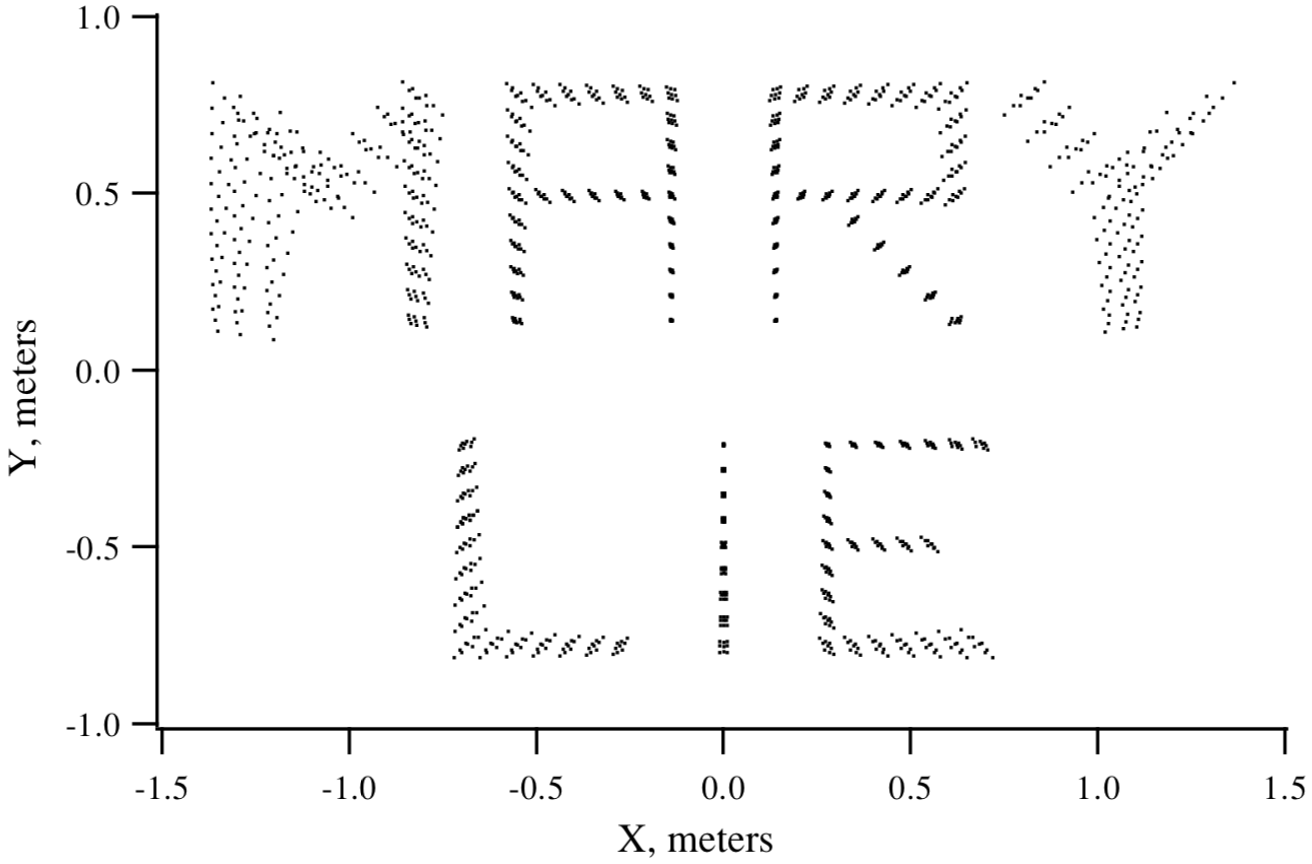
\includegraphics[height=2.75in]{imagenorm}
  \caption{Image of the word \Mary produced by
                  simple imaging system including effect of
                     hard-edge quadrupole fringe fields.}
\end{figure}

\begin{figure}[h]
  \centering
  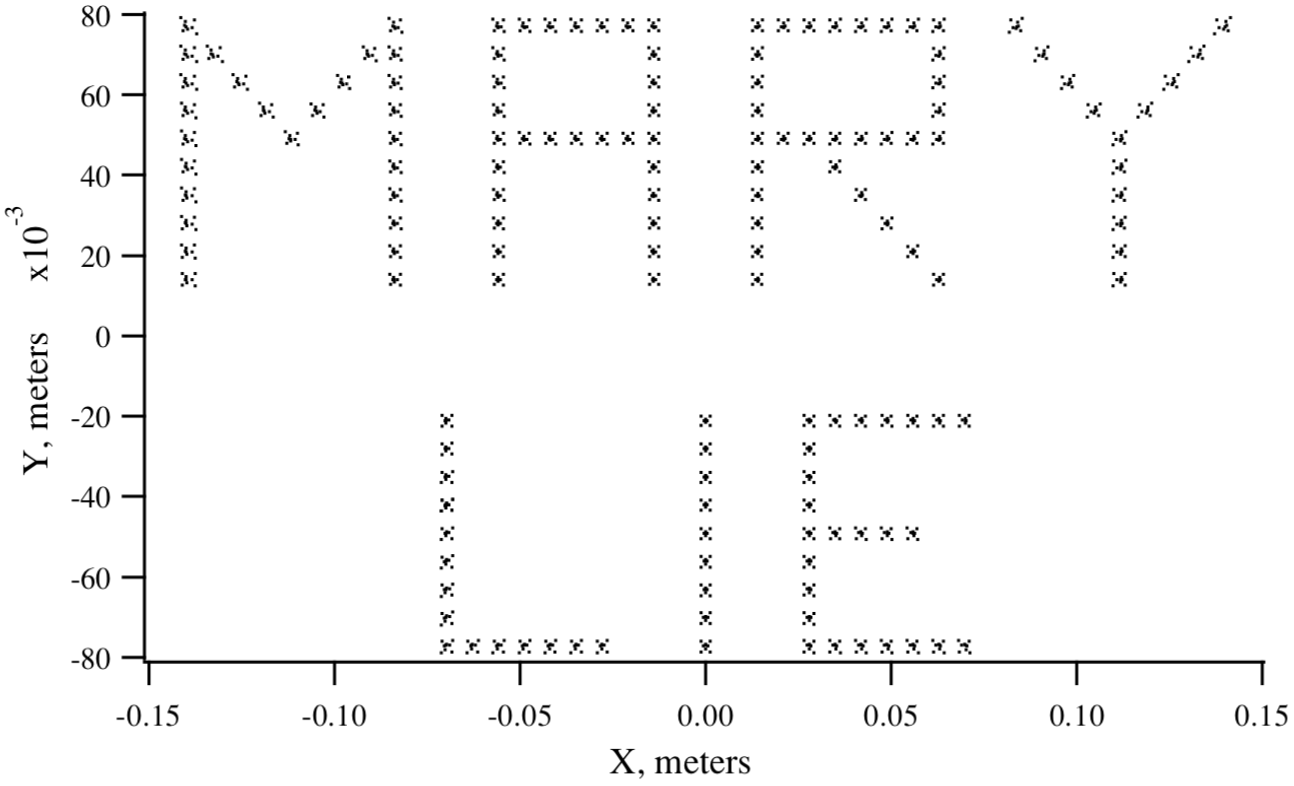
\includegraphics[height=2.5in]{imagesmall}
  \caption{Image of the word \Mary produced
               by the same simple imaging system when the size
                          of the object is reduced.}
\end{figure}

\newpage
\begin{figure}[htp]
  \centering
  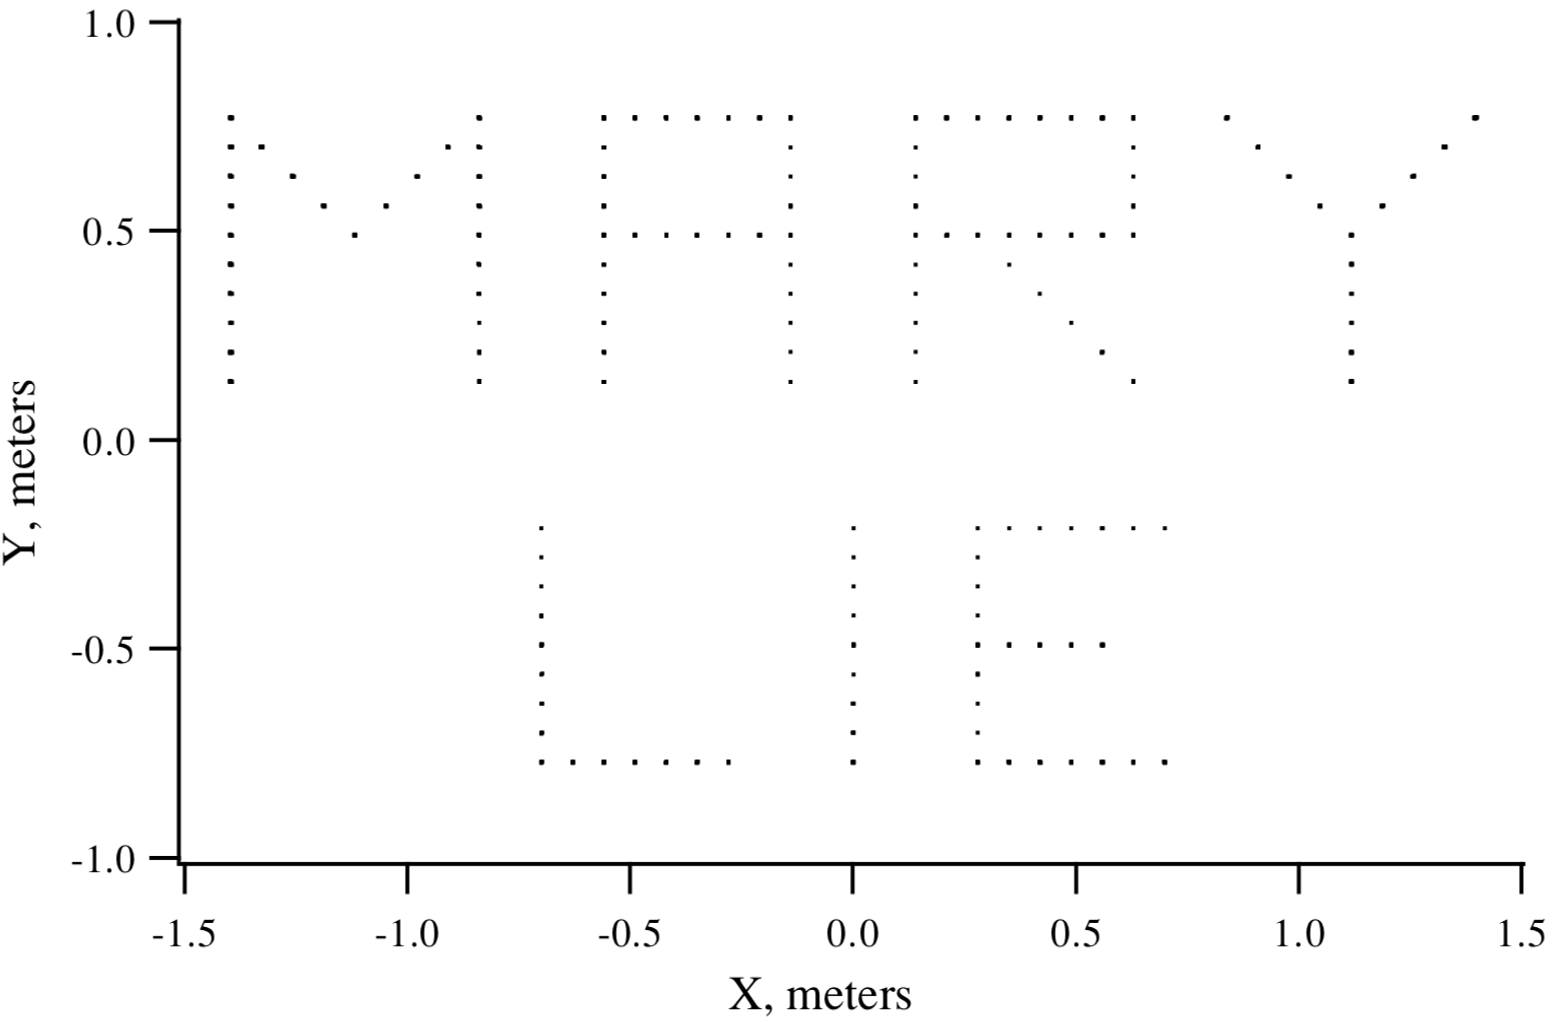
\includegraphics[height=3.25in]{imagenoquad}
  \caption{Image of the word \Mary
                  produced when the effect of quadrupole
                  fringe fields is neglected.}
\end{figure}

{
\footnotesize\tt
\begin{verbatim}
 #comment
  Exhibit 2.3.2.
  This is a study of a simple imaging system with the
  effect of quadrupole fringe fields neglected.
 #beam
   66710.00000000000
   21315.00000000000
   1.000000000000000
   1.000000000000000
 #menu
  dl1      drft
    99.9898870000000
  dl2      drft
    100.000000000000
  ds       drft
    5.00000000000000
  qf1      quad
    10.0000000000000       192.642380000000      0.000000000000000E+00
   0.000000000000000E+00
  qf2      quad
    10.0000000000000       192.642395000000      0.000000000000000E+00
   0.000000000000000E+00
  qd1      quad
    10.0000000000000      -192.642380000000      0.000000000000000E+00
   0.000000000000000E+00
  qd2      quad
    10.0000000000000      -192.642395000000      0.000000000000000E+00
   0.000000000000000E+00
  end      end
  rays     rt
    13.0000000000000       14.0000000000000       5.00000000000000
    1.00000000000000       1.00000000000000      0.000000000000000E+00
  mapout   ptm
    3.00000000000000       3.00000000000000      0.000000000000000E+00
   0.000000000000000E+00   1.00000000000000

  fileout  pmif
    1.00000000000000       12.0000000000000       3.00000000000000
 #lines
  half
      1*dl1         1*qf1         1*ds          1*qd2         2*dl2
&
      1*qf2         1*ds          1*qd1         1*dl1
  image
      2*half
 #lumps
 #loops
 #labor
     1*fileout
     1*image
     1*mapout
     1*end

 matrix for map is :
 9.99856E-01 -1.28018E-06  0.00000E+00  0.00000E+00 0.00000E+00 0.00000E+00
-3.22156E-06  1.00014E+00  0.00000E+00  0.00000E+00 0.00000E+00 0.00000E+00
 0.00000E+00  0.00000E+00  1.00014E+00 -1.28018E-06 0.00000E+00 0.00000E+00
 0.00000E+00  0.00000E+00 -3.22156E-06  9.99856E-01 0.00000E+00 0.00000E+00
 0.00000E+00  0.00000E+00  0.00000E+00  0.00000E+00 1.00000E+00 1.98067E-06
 0.00000E+00  0.00000E+00  0.00000E+00  0.00000E+00 0.00000E+00 1.00000E+00

 nonzero elements in generating polynomial are :

  f( 33)=f( 20 00 01 )=-0.38872686692784D-01
  f( 38)=f( 11 00 01 )= 0.34566885965630D+01
  f( 53)=f( 02 00 01 )=-0.48798663436745D+03
  f( 67)=f( 00 20 01 )=-0.38872615870228D-01
  f( 70)=f( 00 11 01 )=-0.34598333034969D+01
  f( 76)=f( 00 02 01 )=-0.48812740619185D+03
  f( 83)=f( 00 00 03 )=-0.99033373115764D-06
  f( 84)=f( 40 00 00 )=-0.36576395844088D-05
  f( 85)=f( 31 00 00 )= 0.72452798622020D-03
  f( 90)=f( 22 00 00 )=-0.25247349820513D+00
  f( 95)=f( 20 20 00 )=-0.71223902931457D-05
  f( 96)=f( 20 11 00 )=-0.55678664776493D-03
  f( 99)=f( 20 02 00 )=-0.77780590984358D-01
  f(104)=f( 20 00 02 )=-0.97111094673821D-01
  f(105)=f( 13 00 00 )= 0.18656675553303D+02
  f(110)=f( 11 20 00 )= 0.55541554577229D-03
  f(111)=f( 11 11 00 )=-0.22030609589099D+00
  f(114)=f( 11 02 00 )=-0.41123941842952D+01
  f(119)=f( 11 00 02 )= 0.86317322338312D+01
  f(140)=f( 04 00 00 )=-0.78894230698405D+03
  f(145)=f( 02 20 00 )=-0.77722499566606D-01
  f(146)=f( 02 11 00 )= 0.41071535499672D+01
  f(149)=f( 02 02 00 )=-0.62932224711005D+03
  f(154)=f( 02 00 02 )=-0.39715437881394D+03
  f(175)=f( 00 40 00 )=-0.36578660092510D-05
  f(176)=f( 00 31 00 )=-0.72594612592996D-03
  f(179)=f( 00 22 00 )=-0.25265388679573D+00
  f(184)=f( 00 20 02 )=-0.97110897267768D-01
  f(185)=f( 00 13 00 )=-0.18672228901964D+02
  f(190)=f( 00 11 02 )=-0.86342917628377D+01
  f(195)=f( 00 04 00 )=-0.78939756209382D+03
  f(200)=f( 00 02 02 )=-0.39726895527551D+03
  f(209)=f( 00 00 04 )=-0.99033373279231D-06
\end{verbatim}}

\section{Simple Spectrometer}
\label{simplespec}
     The examples of the simple spot forming system and the simple imaging
system both dealt with monoenergtic rays.  This example treats rays with
differing energies.

Consider the simple spectrometer\index{spectrometer} shown in figure 2.4.1 below.  It
consists of a $90^{\circ}$  normal entry and exit dipole bending magnet preceded and
followed by identical drifts.  The system employs a 0.5 Telsa dipole field
strength and is designed to work with 200 MeV electrons.  As indicated in
the figure, the drift lengths have been adjusted so that (in the linear
approximation) the system is focusing (imaging) in the horizontal
direction.  Because the dipole is employed with normal entry and exit, the
system is not focusing in the vertical direction.  That is, the system is
not double focusing.

\begin{figure}[htp]
  \centering
  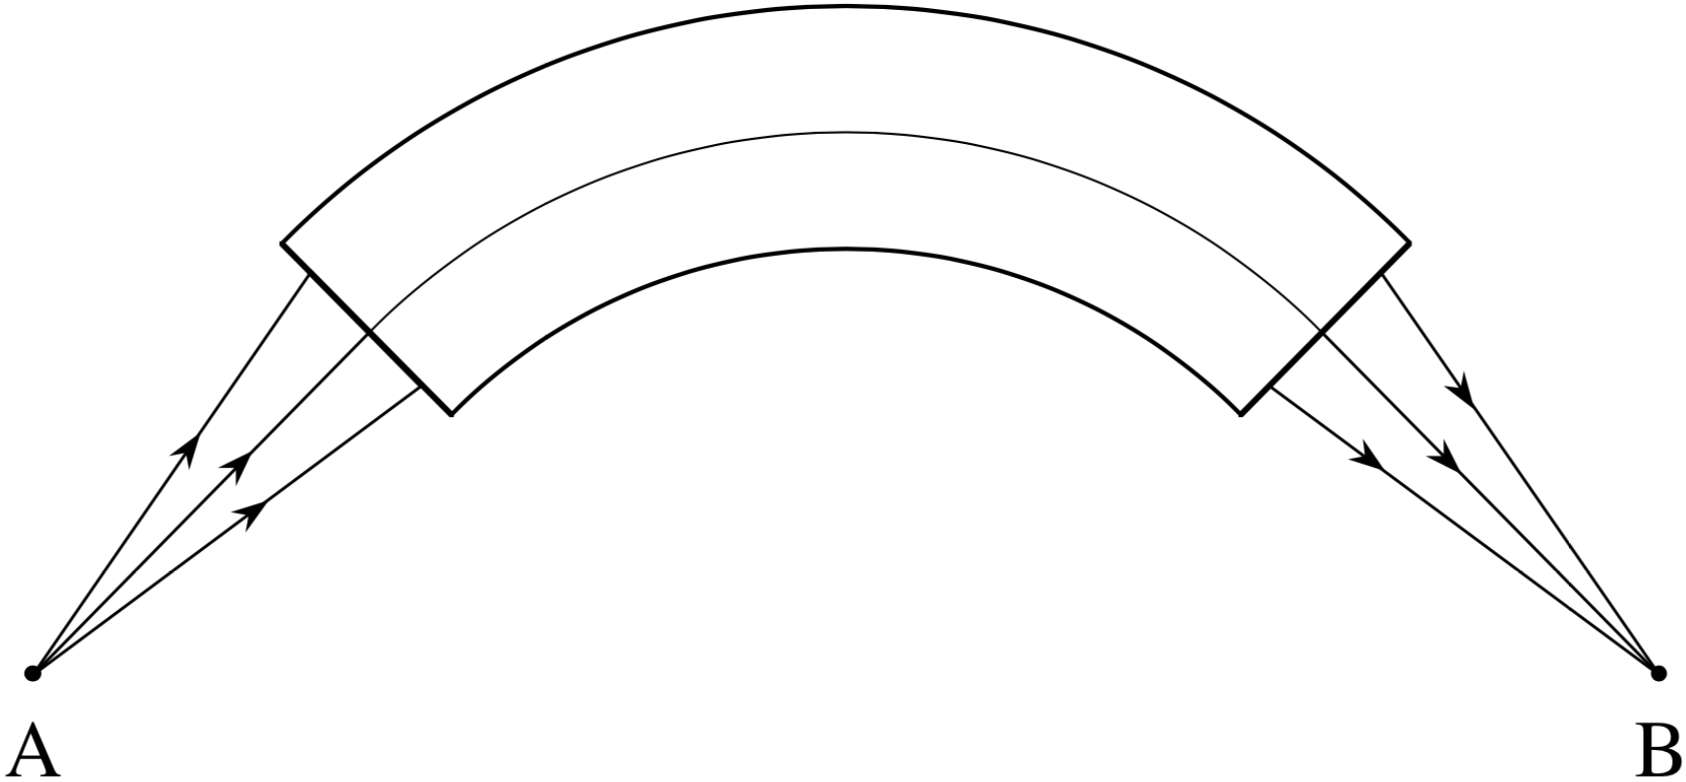
\includegraphics[scale=0.453]{Spectrometer}
  \caption{A simple spectrometer.  Electrons in the
           horizontal plane emanating from point A, and having an
           energy of 200 MeV, are brought to a focus at point B.}
\end{figure}

     The result of a \Mary 3.0 run set up to study this system is shown
below:

{
\footnotesize\tt
\begin{verbatim}
 #comment
  Exhibit 2.4.
  This is a study of a simple electron spectrometer.
 #beam
  0.6688305422661700
   391.3868283459600
   1.000000000000000
   1.000000000000000
 #menu
  dipole   nbnd
    90.0000000000000      0.000000000000000E+00  0.500000000000000
   0.500000000000000       1.00000000000000       1.00000000000000
  end      end
  mapout   ptm
    3.00000000000000       3.00000000000000      0.000000000000000E+00
   0.000000000000000E+00   1.00000000000000
  trmat    ptm
   0.000000000000000E+00  0.000000000000000E+00   3.00000000000000
    3.00000000000000       1.00000000000000
  fileout  pmif
    1.00000000000000       12.0000000000000       3.00000000000000
  rays     rt
    13.0000000000000       14.0000000000000       5.00000000000000
    1.00000000000000       1.00000000000000      0.000000000000000E+00
  dr       drft
    1.33766000000000
 #lines
  spec
      1*dr          1*dipole      1*dr
 #lumps
 #loops
 #labor
     1*fileout
     1*spec
     1*mapout
     1*trmat
     1*rays
     1*end

 matrix for map is :

-9.99999E-01  2.16906E-06 0.00000E+00 0.00000E+00  0.00000E+00 -2.67533E+00
-7.47574E-01 -9.99999E-01 0.00000E+00 0.00000E+00  0.00000E+00 -1.00000E+00
 0.00000E+00  0.00000E+00 1.00000E+00 4.77651E+00  0.00000E+00  0.00000E+00
 0.00000E+00  0.00000E+00 0.00000E+00 1.00000E+00  0.00000E+00  0.00000E+00
 1.00000E+00  2.67533E+00 0.00000E+00 0.00000E+00  1.00000E+00 -7.63506E-01
 0.00000E+00  0.00000E+00 0.00000E+00 0.00000E+00  0.00000E+00  1.00000E+00

 nonzero elements in generating polynomial are :

  f( 28)=f( 30 00 00 )=-0.93144360270528D-01
  f( 29)=f( 21 00 00 )= 0.37378645487843D+00
  f( 33)=f( 20 00 01 )=-0.74757564052220D+00
  f( 34)=f( 12 00 00 )=-0.49999918923267D+00
  f( 38)=f( 11 00 01 )= 0.20000040626018D+01
  f( 39)=f( 10 20 00 )=-0.27943308081159D+00
  f( 40)=f( 10 11 00 )= 0.19218586424872D+01
  f( 43)=f( 10 02 00 )=-0.38044947926129D+01
  f( 48)=f( 10 00 02 )=-0.15000121790723D+01
  f( 49)=f( 03 00 00 )= 0.44588648591172D+00
  f( 53)=f( 02 00 01 )=-0.20064948891860D+01
  f( 54)=f( 01 20 00 )= 0.74757321281106D+00
  f( 55)=f( 01 11 00 )=-0.35707926209417D+01
  f( 58)=f( 01 02 00 )= 0.64267805042870D+01
  f( 63)=f( 01 00 02 )= 0.20065106354604D+01
  f( 67)=f( 00 20 01 )=-0.37378797178870D+00
  f( 70)=f( 00 11 01 )= 0.25708038645726D+01
  f( 76)=f( 00 02 01 )=-0.64268055010847D+01
  f( 83)=f( 00 00 03 )=-0.89179523414583D+00
  f( 84)=f( 40 00 00 )=-0.52224150326159D-01
  f( 85)=f( 31 00 00 )= 0.27943262770116D+00
  f( 89)=f( 30 00 01 )=-0.37257842445493D+00
  f( 90)=f( 22 00 00 )=-0.65412546263926D+00
  f( 94)=f( 21 00 01 )= 0.16820436001359D+01
  f( 95)=f( 20 20 00 )=-0.52224192667846D-01
  f( 96)=f( 20 11 00 )= 0.41914950793973D+00
  f( 99)=f( 20 02 00 )=-0.13347157761221D+01
  f(104)=f( 20 00 02 )=-0.13082632129161D+01
  f(105)=f( 13 00 00 )= 0.74999817577475D+00
  f(109)=f( 12 00 01 )=-0.30000042696722D+01
  f(110)=f( 11 20 00 )=-0.29921602979568D+00
  f(111)=f( 11 11 00 )= 0.97520757686635D+00
  f(114)=f( 11 02 00 )= 0.23370935338336D+01
  f(119)=f( 11 00 02 )= 0.45000280175421D+01
  f(123)=f( 10 20 01 )=-0.55886786323843D+00
  f(126)=f( 10 11 01 )= 0.34170158616280D+01
  f(132)=f( 10 02 01 )=-0.78753142617592D+01
  f(139)=f( 10 00 03 )=-0.20000280110477D+01
  f(140)=f( 04 00 00 )=-0.50162182216850D+00
  f(144)=f( 03 00 01 )= 0.21179659236963D+01
  f(145)=f( 02 20 00 )= 0.40024916288944D+00
  f(146)=f( 02 11 00 )=-0.19117958694217D+01
  f(149)=f( 02 02 00 )=-0.16758500076646D+01
  f(154)=f( 02 00 02 )=-0.48490507651341D+01
  f(158)=f( 01 20 01 )= 0.72111221900917D+00
  f(161)=f( 01 11 01 )=-0.40517040534188D+01
  f(167)=f( 01 02 01 )= 0.12766450201372D+02
  f(174)=f( 01 00 03 )= 0.36786182170241D+01
  f(175)=f( 00 40 00 )=-0.52224192667846D-01
  f(176)=f( 00 31 00 )= 0.49889908271819D+00
  f(179)=f( 00 22 00 )=-0.18588566566436D+01
  f(184)=f( 00 20 02 )=-0.65413213721516D+00
  f(185)=f( 00 13 00 )= 0.31876425698809D+01
  f(190)=f( 00 11 02 )= 0.38208251163414D+01
  f(195)=f( 00 04 00 )=-0.28789752521441D+01
  f(200)=f( 00 02 02 )=-0.94839470235307D+01
  f(209)=f( 00 00 04 )=-0.10590132322744D+01

 nonzero elements in second order matrix are :

  t1(  7)=t1( 20 00 00 )=-0.37378675793264D+00
  t1(  8)=t1( 11 00 00 )=-0.99999918923235D+00
  t1( 12)=t1( 10 00 01 )=-0.20000056841418D+01
  t1( 13)=t1( 02 00 00 )=-0.13376594577343D+01
  t1( 17)=t1( 01 00 01 )=-0.40129908629061D+01
  t1( 18)=t1( 00 20 00 )=-0.74757321281106D+00
  t1( 19)=t1( 00 11 00 )=-0.35707938944926D+01
  t1( 22)=t1( 00 02 00 )=-0.64267835458532D+01
  t1( 27)=t1( 00 00 02 )=-0.20065122622686D+01
  t2(  7)=t2( 20 00 00 )=-0.13877787807814D-16
  t2(  8)=t2( 11 00 00 )=-0.13877787807814D-16
  t2( 12)=t2( 10 00 01 )=-0.27755575615629D-16
  t2( 13)=t2( 02 00 00 )=-0.50000000000000D+00
  t2( 17)=t2( 01 00 01 )=-0.10000024366857D+01
  t2( 18)=t2( 00 20 00 )=-0.27943308081159D+00
  t2( 19)=t2( 00 11 00 )=-0.74757290975685D+00
  t2( 22)=t2( 00 02 00 )=-0.99999918923267D+00
  t2( 27)=t2( 00 00 02 )=-0.32474612975120D-05
  t3(  9)=t3( 10 10 00 )=-0.74757290975685D+00
  t3( 10)=t3( 10 01 00 )=-0.15707934317094D+01
  t3( 14)=t3( 01 10 00 )=-0.35707938944926D+01
  t3( 15)=t3( 01 01 00 )=-0.42023767872970D+01
  t3( 21)=t3( 00 10 01 )=-0.10000024366857D+01
  t3( 24)=t3( 00 01 01 )= 0.57413261902772D+00
  t4(  9)=t4( 10 10 00 )=-0.55886616162317D+00
  t4( 10)=t4( 10 01 00 )=-0.19218586424872D+01
  t4( 14)=t4( 01 10 00 )=-0.14951464256221D+01
  t4( 15)=t4( 01 01 00 )=-0.35707926209417D+01
  t4( 21)=t4( 00 10 01 )=-0.74757594357739D+00
  t4( 24)=t4( 00 01 01 )=-0.25708038645726D+01
  t5(  7)=t5( 20 00 00 )= 0.37378766873350D+00
  t5(  8)=t5( 11 00 00 )= 0.10000016259161D+01
  t5( 12)=t5( 10 00 01 )= 0.10000121790723D+01
  t5( 13)=t5( 02 00 00 )= 0.20064959737214D+01
  t5( 17)=t5( 01 00 01 )= 0.26753536674612D+01
  t5( 18)=t5( 00 20 00 )= 0.37378797178870D+00
  t5( 19)=t5( 00 11 00 )= 0.10000024366857D+01
  t5( 22)=t5( 00 02 00 )= 0.26753286879845D+01
  t5( 27)=t5( 00 00 02 )= 0.66887561213844D+00

 nonzero elements in third order matrix are :

  u1( 28)=u1( 30 00 00 )=-0.27943285425628D+00
  u1( 29)=u1( 21 00 00 )=-0.11213584554734D+01
  u1( 33)=u1( 20 00 01 )=-0.14951509779892D+01
  u1( 34)=u1( 12 00 00 )=-0.19999963515485D+01
  u1( 38)=u1( 11 00 01 )=-0.50000097511198D+01
  u1( 39)=u1( 10 20 00 )=-0.27943308081159D+00
  u1( 40)=u1( 10 11 00 )=-0.14951464256221D+01
  u1( 43)=u1( 10 02 00 )=-0.40707942998761D+01
  u1( 48)=u1( 10 00 02 )=-0.35000272002167D+01
  u1( 49)=u1( 03 00 00 )=-0.20064878309384D+01
  u1( 53)=u1( 02 00 01 )=-0.60194852098259D+01
  u1( 54)=u1( 01 20 00 )= 0.80049927785190D+00
  u1( 55)=u1( 01 11 00 )= 0.46089928282951D+01
  u1( 58)=u1( 01 02 00 )=-0.14759688968051D+01
  u1( 63)=u1( 01 00 02 )=-0.86948546235550D+01
  u1( 67)=u1( 00 20 01 )=-0.14951512810444D+01
  u1( 70)=u1( 00 11 01 )=-0.85708168631484D+01
  u1( 76)=u1( 00 02 01 )=-0.17986352150007D+02
  u1( 83)=u1( 00 00 03 )=-0.26753683263812D+01
  u2( 28)=u2( 30 00 00 )=-0.20816681711722D-16
  u2( 33)=u2( 20 00 01 )=-0.14571677198205D-15
  u2( 34)=u2( 12 00 00 )=-0.20816681711722D-16
  u2( 38)=u2( 11 00 01 )= 0.11102230246252D-15
  u2( 39)=u2( 10 20 00 )=-0.69388939039072D-17
  u2( 40)=u2( 10 11 00 )=-0.27755575615629D-16
  u2( 43)=u2( 10 02 00 )=-0.55511151231258D-15
  u2( 48)=u2( 10 00 02 )=-0.61062266354384D-15
  u2( 49)=u2( 03 00 00 )=-0.49999959461617D+00
  u2( 53)=u2( 02 00 01 )=-0.50000162372801D+00
  u2( 55)=u2( 01 11 00 )= 0.74757351586528D+00
  u2( 58)=u2( 01 02 00 )= 0.49999959461617D+00
  u2( 63)=u2( 01 00 02 )=-0.10000089316083D+01
  u2( 67)=u2( 00 20 01 )=-0.27943398825823D+00
  u2( 70)=u2( 00 11 01 )=-0.14951506749340D+01
  u2( 76)=u2( 00 02 01 )=-0.20000040626022D+01
  u2( 83)=u2( 00 00 03 )=-0.32474718438813D-05
  u3( 30)=u3( 20 10 00 )= 0.16653345369377D-15
  u3( 31)=u3( 20 01 00 )=-0.37378645487842D+00
  u3( 35)=u3( 11 10 00 )= 0.42671126479216D+00
  u3( 36)=u3( 11 01 00 )=-0.14292029772358D+01
  u3( 42)=u3( 10 10 01 )=-0.14951506749340D+01
  u3( 45)=u3( 10 01 01 )=-0.61416043756418D+01
  u3( 50)=u3( 02 10 00 )=-0.92920500415430D+00
  u3( 51)=u3( 02 01 00 )=-0.29623833617786D+01
  u3( 57)=u3( 01 10 01 )=-0.60000142721308D+01
  u3( 60)=u3( 01 01 01 )=-0.17768425853934D+02
  u3( 64)=u3( 00 30 00 )=-0.27943285425628D+00
  u3( 65)=u3( 00 21 00 )=-0.13347140878695D+01
  u3( 68)=u3( 00 12 00 )=-0.25707905366266D+01
  u3( 73)=u3( 00 10 02 )=-0.20000146157580D+01
  u3( 74)=u3( 00 03 00 )=-0.76352754186107D+00
  u3( 79)=u3( 00 01 02 )=-0.48712382645289D+01
  u4( 30)=u4( 20 10 00 )=-0.12143064331838D-16
  u4( 31)=u4( 20 01 00 )=-0.55886616162317D+00
  u4( 35)=u4( 11 10 00 )= 0.87786491384764D+00
  u4( 36)=u4( 11 01 00 )=-0.10684345547215D+01
  u4( 42)=u4( 10 10 01 )=-0.55886797651645D+00
  u4( 45)=u4( 10 01 01 )=-0.41645921082604D+01
  u4( 50)=u4( 02 10 00 )= 0.80049802272480D+00
  u4( 51)=u4( 02 01 00 )=-0.17146015460171D+01
  u4( 57)=u4( 01 10 01 )=-0.10684370723398D+01
  u4( 60)=u4( 01 01 01 )=-0.95708180262792D+01
  u4( 64)=u4( 00 30 00 )=-0.20889677067138D+00
  u4( 65)=u4( 00 21 00 )=-0.12772310196927D+01
  u4( 68)=u4( 00 12 00 )=-0.26694299940634D+01
  u4( 73)=u4( 00 10 02 )=-0.74758079901346D+00
  u4( 74)=u4( 00 03 00 )=-0.25707934317102D+01
  u4( 79)=u4( 00 01 02 )=-0.45708327407763D+01
  u5( 28)=u5( 30 00 00 )= 0.93144662752742D-01
  u5( 29)=u5( 21 00 00 )= 0.37378766873350D+00
  u5( 33)=u5( 20 00 01 )= 0.11213693785478D+01
  u5( 34)=u5( 12 00 00 )= 0.10000020313009D+01
  u5( 38)=u5( 11 00 01 )= 0.40000267991940D+01
  u5( 39)=u5( 10 20 00 )= 0.55886774996041D+00
  u5( 40)=u5( 10 11 00 )= 0.19218642775287D+01
  u5( 43)=u5( 10 02 00 )= 0.22337069932108D+01
  u5( 48)=u5( 10 00 02 )= 0.25000422192713D+01
  u5( 49)=u5( 03 00 00 )= 0.17835517356330D+01
  u5( 53)=u5( 02 00 01 )= 0.60195177898336D+01
  u5( 54)=u5( 01 20 00 )= 0.11213630062007D+01
  u5( 55)=u5( 01 11 00 )= 0.15707977220230D+01
  u5( 58)=u5( 01 02 00 )= 0.23191094090778D+01
  u5( 63)=u5( 01 00 02 )= 0.60195775186149D+01
  u5( 67)=u5( 00 20 01 )= 0.11213696816060D+01
  u5( 70)=u5( 00 11 01 )= 0.45708292655895D+01
  u5( 76)=u5( 00 02 01 )= 0.83386436657300D+01
  u5( 83)=u5( 00 00 03 )= 0.15606846026334D+01
\end{verbatim}}


     The {\em \#menu} component of the Master Input File contains, among other
entries, the element {\em dipole}.  The first two parameters under this element
specify the dipole bend angle and strength, respectively.  The remaining
two parameters (both set equal to +1 in this example) indicate that the
dipole is to be treated as having hard-edge leading and trailing fringe
fields.  The {\em \#lines} component of the Master Input File defines the simple
spectrometer in terms of the line called {\em spec}.  The key entries in the
{\em \#labor} component are {\em spec}, {\em mapout}, {\em tmat}, and {\em rays}.  The entry {\em spec } calls
for the computation of the transfer map described by the line {\em spec}.  The
command {\em mapout } calls for the printing of the transfer map for the system.
The command {\em tmat } calls for the printing of the second- and third-order
transfer matrices for the system.  Finally, {\em rays } produces a ray trace.

     There are several observations to be made about the \Mary output.
First, note that the 1,2 component of the transfer matrix vanishes, and the
3,4 component does not.  Thus the system is indeed imaging in the
horizontal plane, but not in the vertical plane.  Second, note that the 1,6
component of the transfer matrix is nonzero.  Consequently, the system is
dispersive as desired for a spectrometer.  Finally, observe that there are
a large number of entries in the generating polynomial describing the
nonlinear behavior of the system.  As a result, the system has a large
number of second and third order aberrations.  Many of these aberrations
arise primarily from the dipole fringe fields.

     It will be shown in a later section that aberrations are completely
and most compactly described in terms of the Lie algebraic generating
polynomial for the nonlinear portion of the transfer map.  Indeed, second
order aberrations are described by the monomials numbered 28 through 83,
and third order aberrations are described by the monomials numbered 84
through 209.  However, as also will be shown later, it is possible as well
to characterize a transfer map in terms of a Taylor series expansion.  When
this is done through third order, there is a set of coefficients $T_{ijk}$    (the
so-called T matrix or second-order transfer matrix) for the quadratic
terms, and a set of coefficients $U_{ijkl}$     for the cubic terms.

     If desired, \Mary can be used to produce these Taylor series coefficients.
In this particular \Mary run, the second- and third-order
transfer matrix for the simple spectrometer have been produced as a result
of the command {\em tmat}. Note that these matrices fill several pages.  By
contrast, the Lie algebraic representation of all the same information
requires only a single page.  Consequently, preliminary (and perhaps most)
analyses of the importance of aberrations are most easily made using the
Lie algebraic representation.

     How well does this simple spectrometer work?  To study this question,
two sets of rays may be launched from the point A of figure 2.4.1.  The
first set is selected to have $P_{\tau}= 5\times 10^{-5}$ and 25 different combinations
of $P_x$ and $P_y$  values.  The second set is selected to have
$P_{\tau}=-5\times 10^{-5}$,
and the same combination of $P_x$  and $P_y$  values.  (As indicated earlier, and
will be described later, the quantity $P_{\tau}$  is related to energy deviation.)
The phase-space coordinates for all these rays are stored in an initial
condition file.  The first few lines of this file are shown below:
\vspace{5mm}

First few lines of  initial condition file for spectrometer ray traces
\begin{footnotesize}
\begin{tt}
\begin{tabbing}
-1.699\=89E-07 -4.012\=00E-04 -9.380\=35E-08 -5.491\=85E-05 9.898\=83E-06 0.000\= \kill
\>$X$ \>$P_x$ \>$Y$ \>$P_y$ \>$\tau$ \>$P_{\tau}$
\end{tabbing}
\end{tt}
\vspace{-5mm}
\begin{verbatim}
0.0000E+00  -0.4000E-02  0.0000E+00  -0.4000E-02  0.0000E+00  0.5000E-04
0.0000E+00  -0.4000E-02  0.0000E+00  -0.2000E-02  0.0000E+00  0.5000E-04
0.0000E+00  -0.4000E-02  0.0000E+00   0.0000E+00  0.0000E+00  0.5000E-04
0.0000E+00  -0.4000E-02  0.0000E+00   0.2000E-02  0.0000E+00  0.5000E-04
0.0000E+00  -0.4000E-02  0.0000E+00   0.4000E-02  0.0000E+00  0.5000E-04
\end{verbatim}
\end{footnotesize}

     Note that the X, Y, and $\tau$ coordinates of all rays are taken to be
zero. This is because the point A has been selected to lie on the ``design
orbit'' or ``chief ray'' for the spectrometer.  Also, the $P_x$  and $P_y$  values
have been selected from a square array.  Figure 2.4.2 below shows the result
of plotting the second and fourth (the $P_x$  and $P_y$  phase-space coordinates)
of the initial condition file.

     Now suppose \Mary is used to trace these two sets of rays through
the spectrometer to the final point B\@.  Figure 2.4.3 shows the result
obtained in the $X,Y$ plane, and figure 2.4.4 shows the same final rays in
terms of the variables $P_{\tau}$  and $X$.


     Inspection of figures 2.4.3 and 2.4.4 shows that the rays arrive at
approximately two horizontal ($X$) locations depending on their $P_{\tau}$  values.
Thus, the system is horizontally focusing as expected.  Moreover, there is
a wide spread of $Y$ values since the system is not vertically focusing.
Finally, there is some spread in the two horizontal arrival values
depending on the $P_x$  and $P_y$  values.  It can be shown that this spread arises
primarily from second-order aberrations described by the coefficients
numbered 49 and 58 in the Lie algebraic generating polynomial for the total
transfer map.

     The observant reader may wonder why Fig. 2.4.3 appears to have only 30
points as the result of tracing 50 rays.  The explanation is that the
arrival point of a ray is nearly the same for corresponding  initial $P_x$
values.

\begin{figure}[hbp]
  \centering
  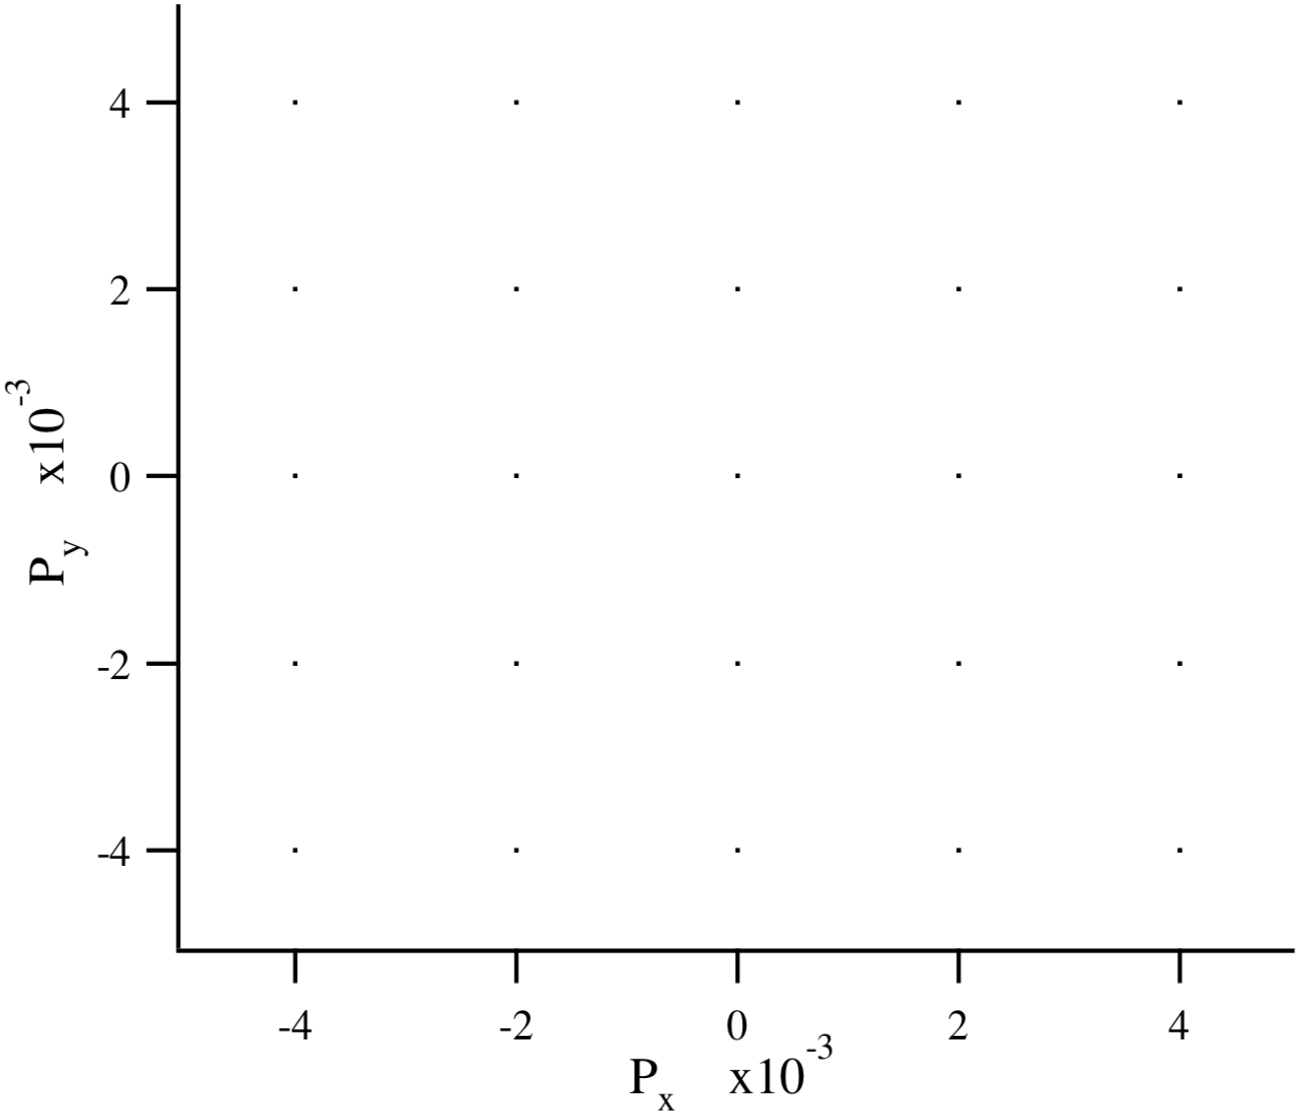
\includegraphics[scale=0.453]{espec}
  \caption{Plot of Initial Conditions for
                Incoming Rays of the Simple Spectrometer.}
\end{figure}

\begin{figure}[hbp]
  \centering
  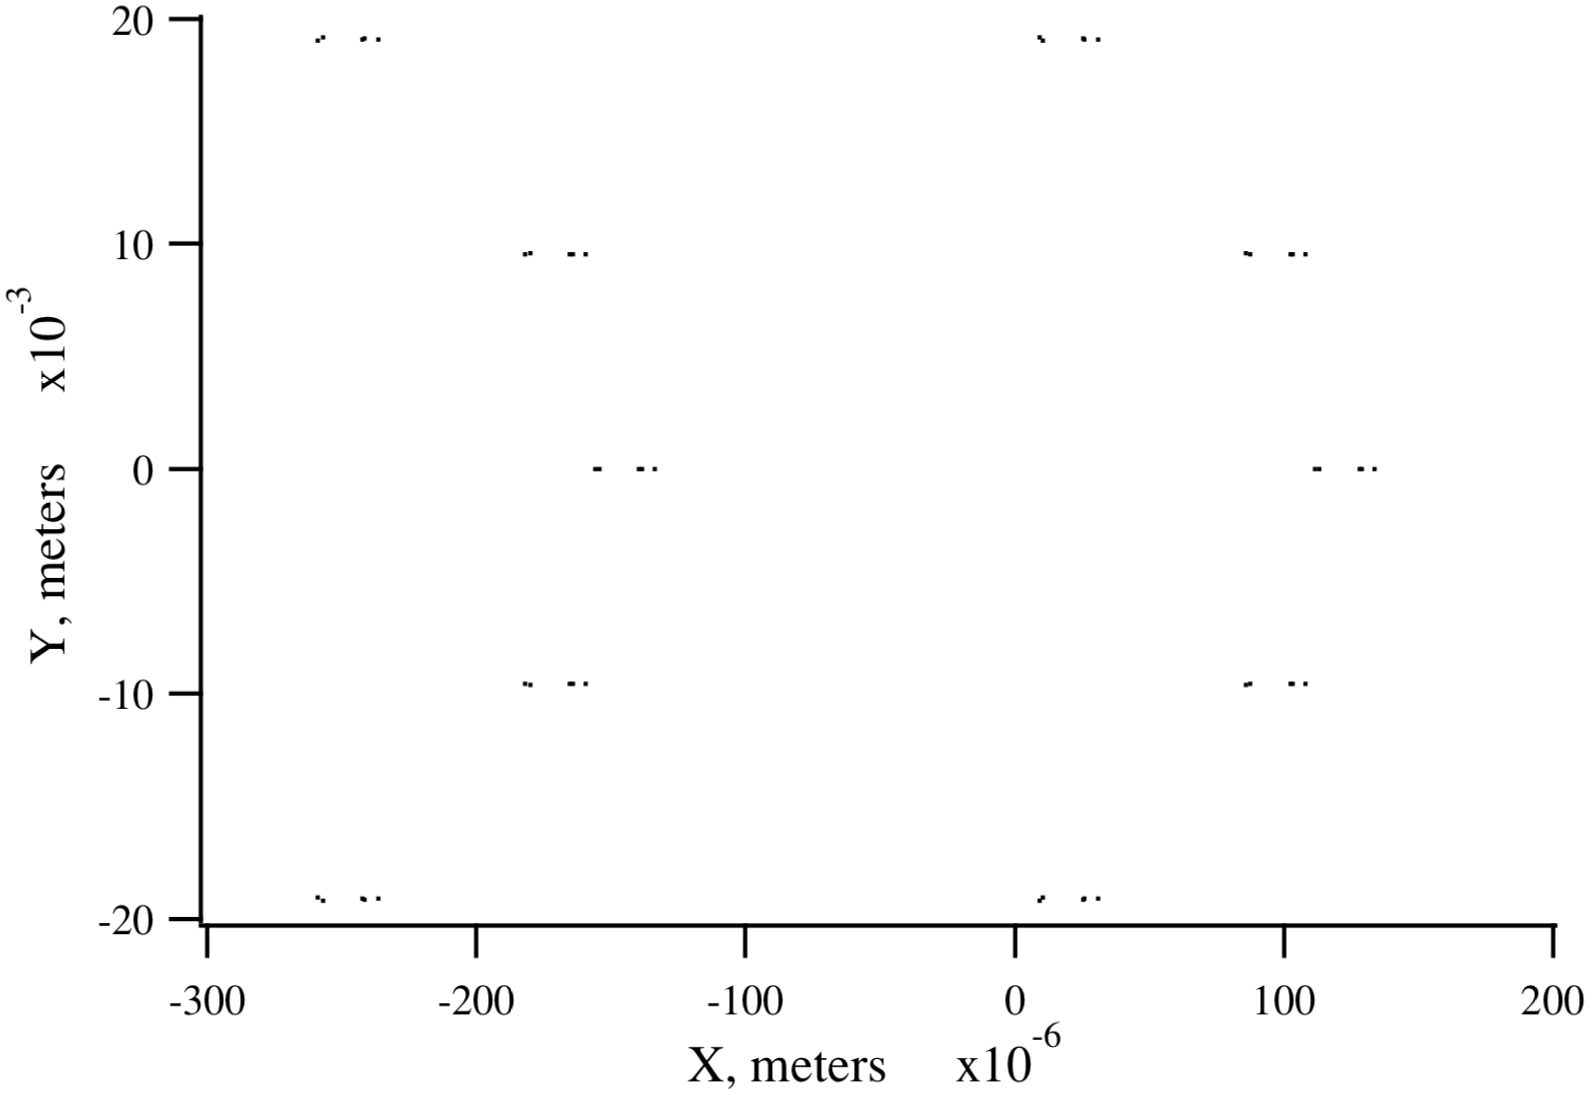
\includegraphics[scale=0.453]{especnorm1}
  \caption{Plot of the pattern produced at the focus B of
        the spectrometer as the result of two sets of incoming rays.}
\end{figure}
\clearpage

\begin{figure}[hbp]
  \centering
  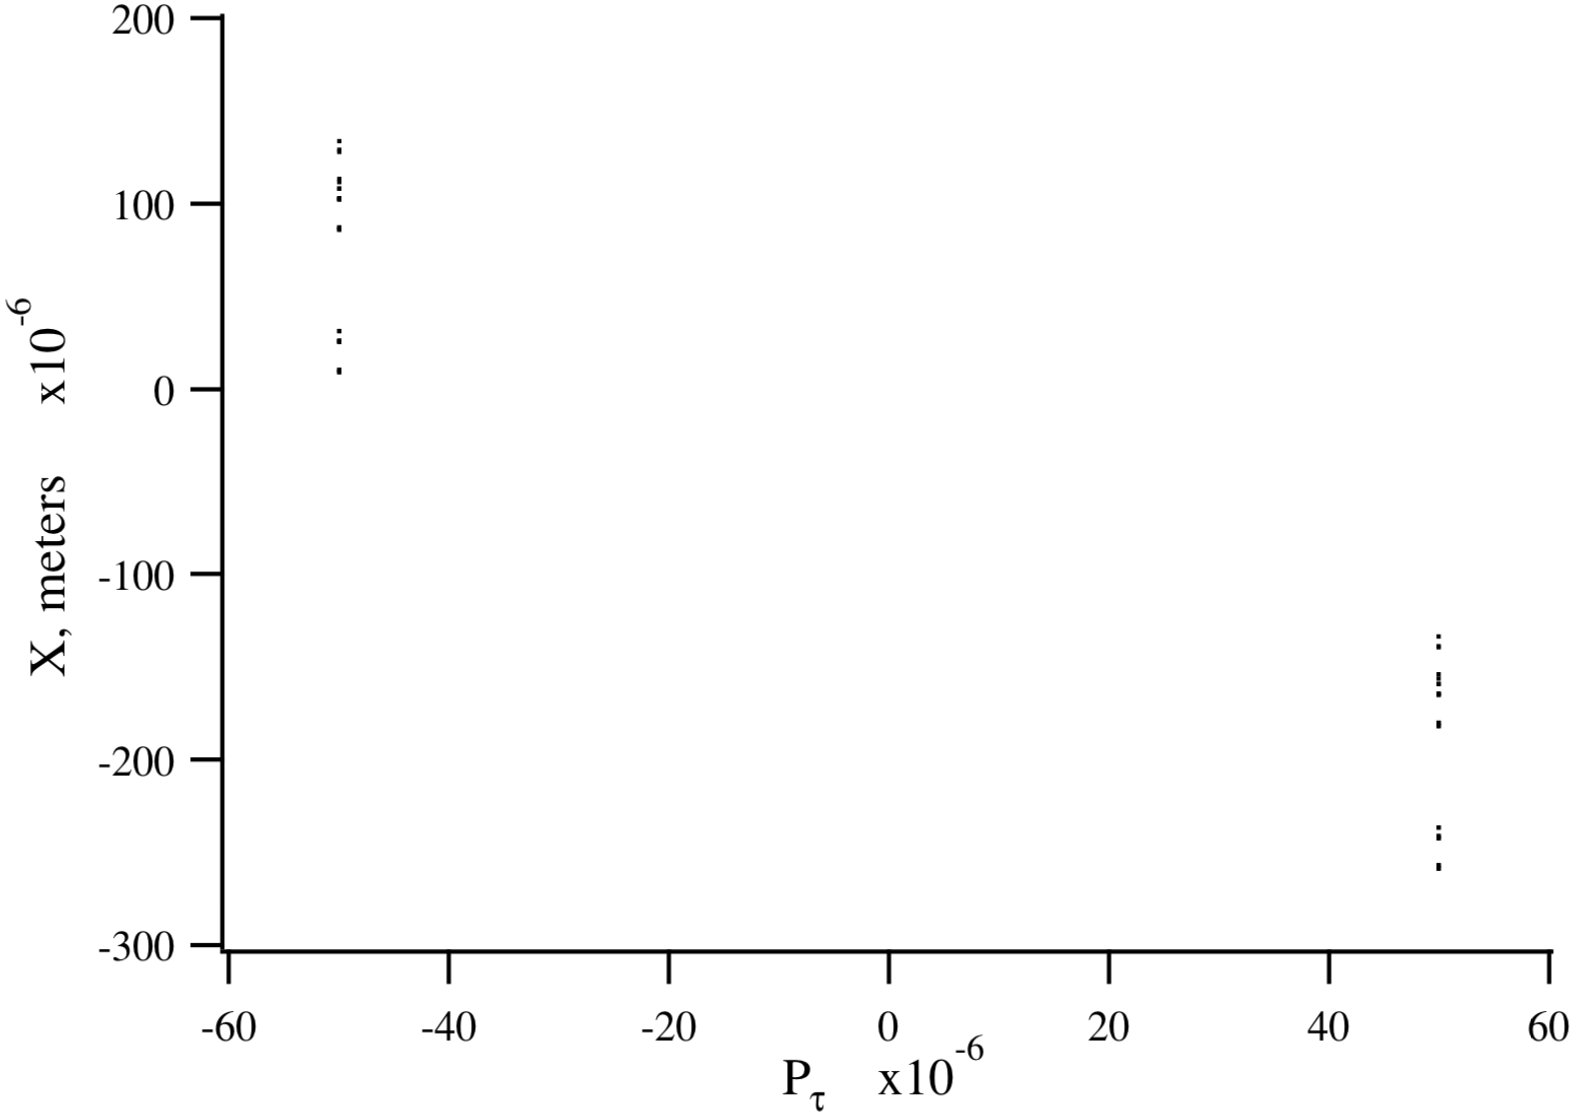
\includegraphics[scale=0.453]{especnorm2}
  \caption{Horizontal arrival point $x$ of final rays
            as a function of energy deviation.}
\end{figure}

As can be seen from either of figures 2.4.3 and 2.4.4, the two sets of rays
with different values of $P_{\tau}$  are well separated in $X$.  Therefore, the
spectrometer has been able to resolve the two different values of $P_{\tau}$.
Now suppose the angular spread of the incoming rays is increased by a
factor of 1.5 so that $P_x$, $P_y$  now reach the extreme values  .006, and
suppose the two $P_{\tau}$  values are the same as before.  Figures 2.4.5
and 2.4.6 show the
result of ray tracing for this case.  Evidently, the $X$ values of the two
sets of rays now overlap due to aberration effects.  Correspondingly, the
two $P_{\tau}$  values are no longer resolved.


\begin{figure}[hbp]
  \centering
  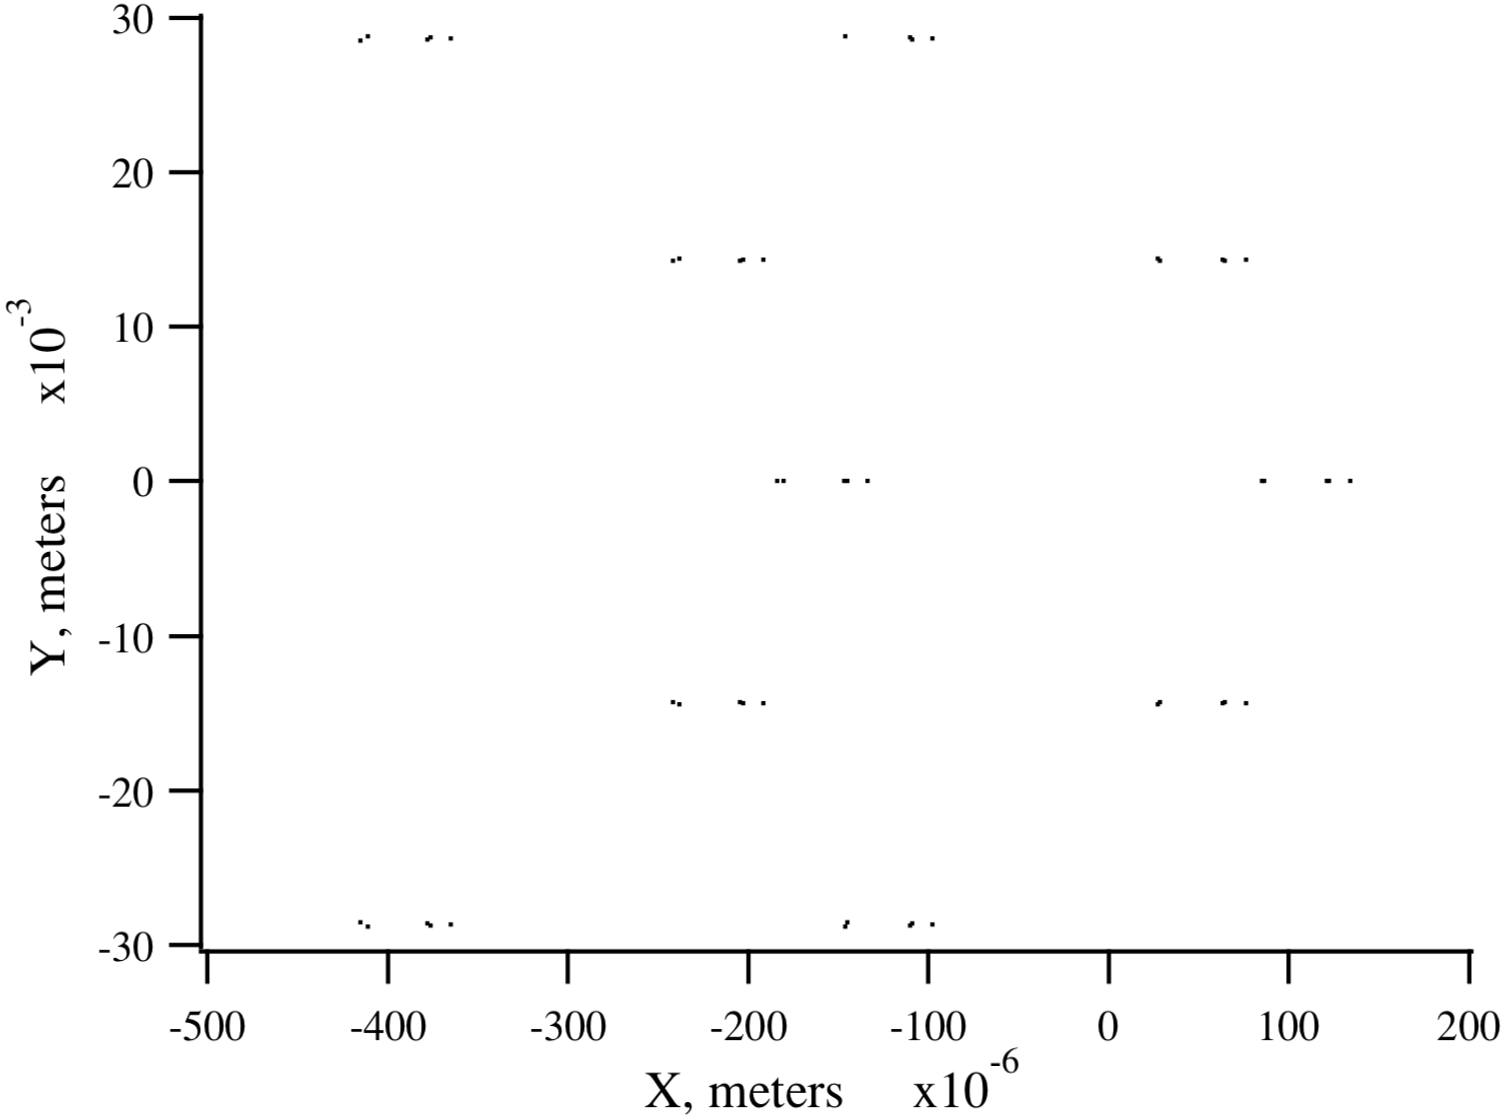
\includegraphics[scale=0.453]{especwide1}
  \caption{Plot of the final ray pattern produced at B
          when the angular spread of the incoming rays is increased.}
\end{figure}


\begin{figure}[hbp]
  \centering
  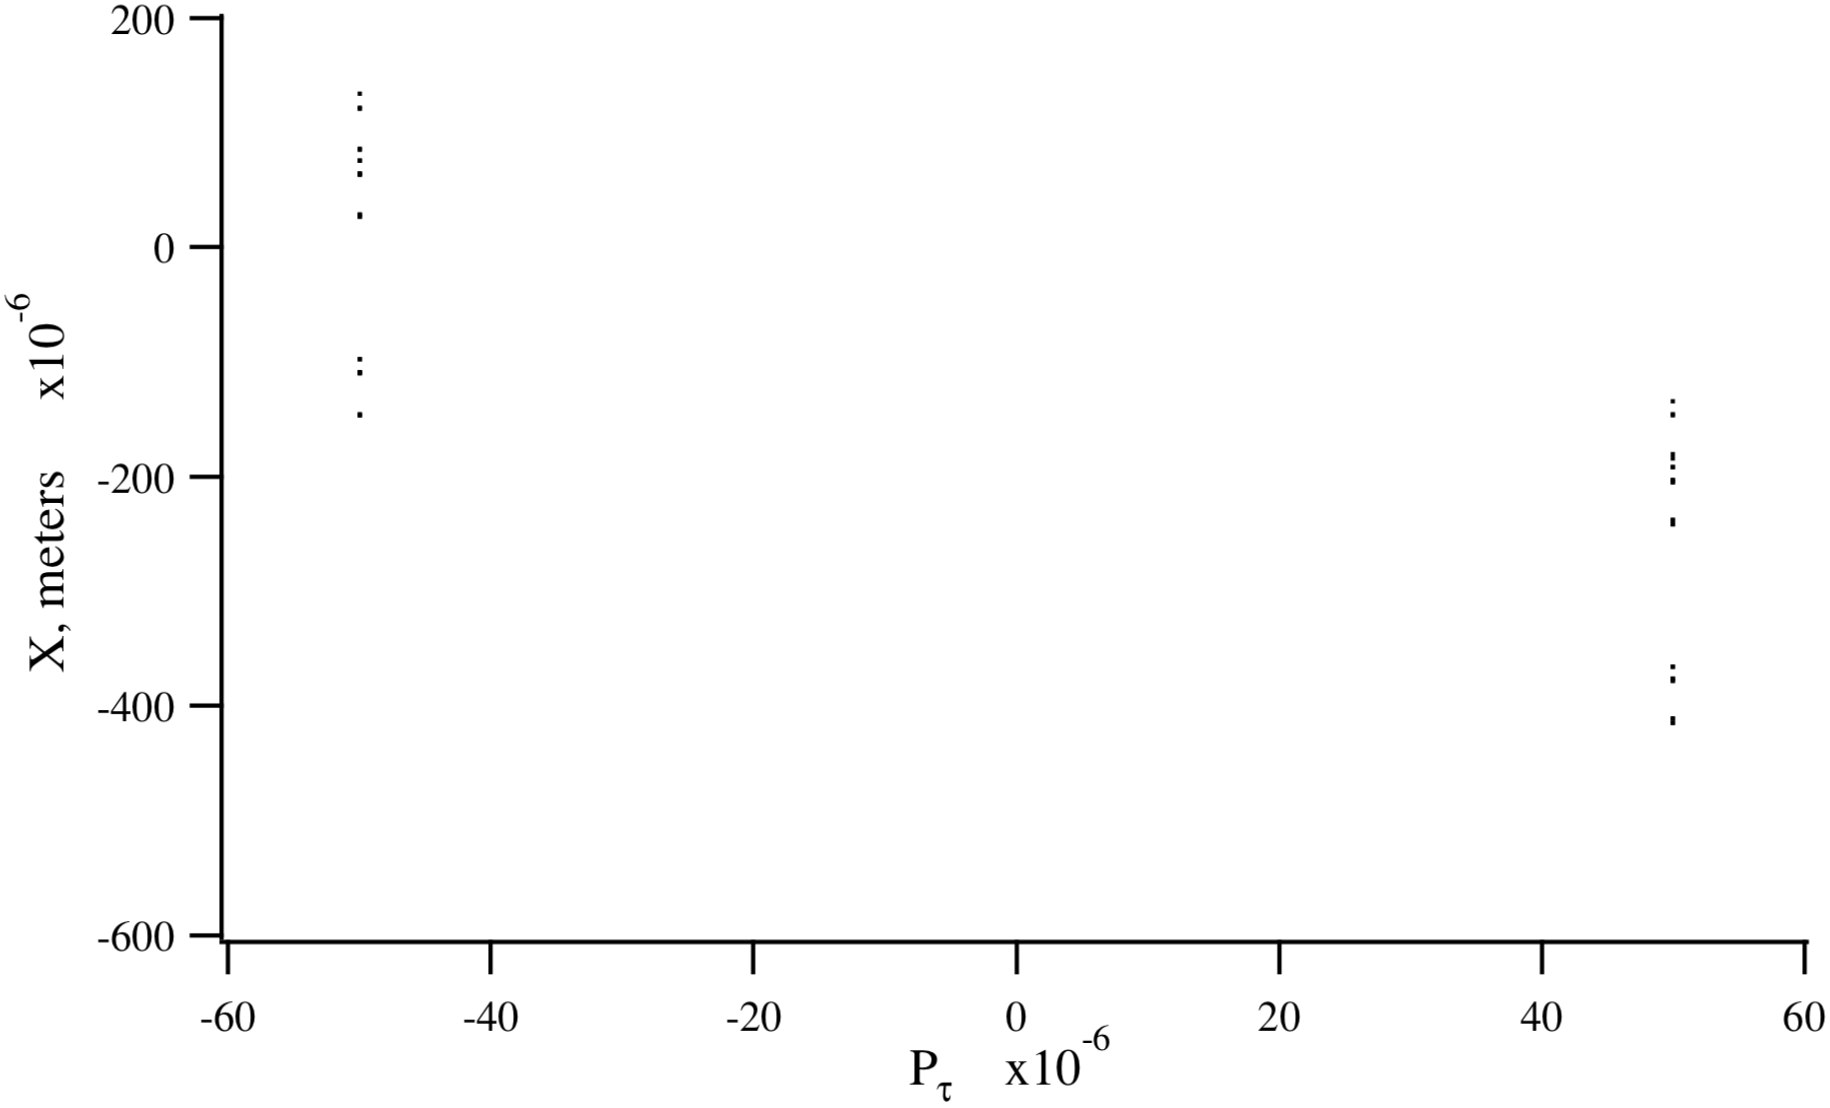
\includegraphics[scale=0.453]{especwide2}
  \caption{Horizontal arrival point $x$ of final rays
           as a function of energy deviation in the case where
           the angular spread of the incoming rays is increased.}
\end{figure}
\clearpage

\section{Small Static Storage Ring}
\label{staticstorage}
     The examples of the simple spot forming system, the simple imaging
system, and the simple spectrometer all dealt with single pass systems.
They were therefore not concerned with the long-term behavior of
trajectories.  By contrast, this example treats a circulating storage
system for which long-term behavior is of paramount importance.

     Consider the small Proton Storage Ring\index{storage ring} (called the PSR and similar to that at the Los
Alamos National Laboratory) shown in figure 2.5.1 below.  It is designed to
store protons with a nominal energy of 800 MeV using $\mbox{H}^-$  injection, and is
arranged as a ten-sided separated function lattice consisting of straight
sections and bends.  The lattice is composed entirely of dipoles,
quadrupoles, and drifts with the exception of two pairs of sextupoles.
When these sextupoles are turned off, the lattice has ten identical
periods.  When the sextupoles are turned on, the symmetry of the lattice is
reduced.  Inspection of figure 2.5.1 shows that in this latter case the
lattice can be viewed as consisting of two identical halves, and thus it
has two identical periods.

\begin{figure}[hbp]
  \centering
  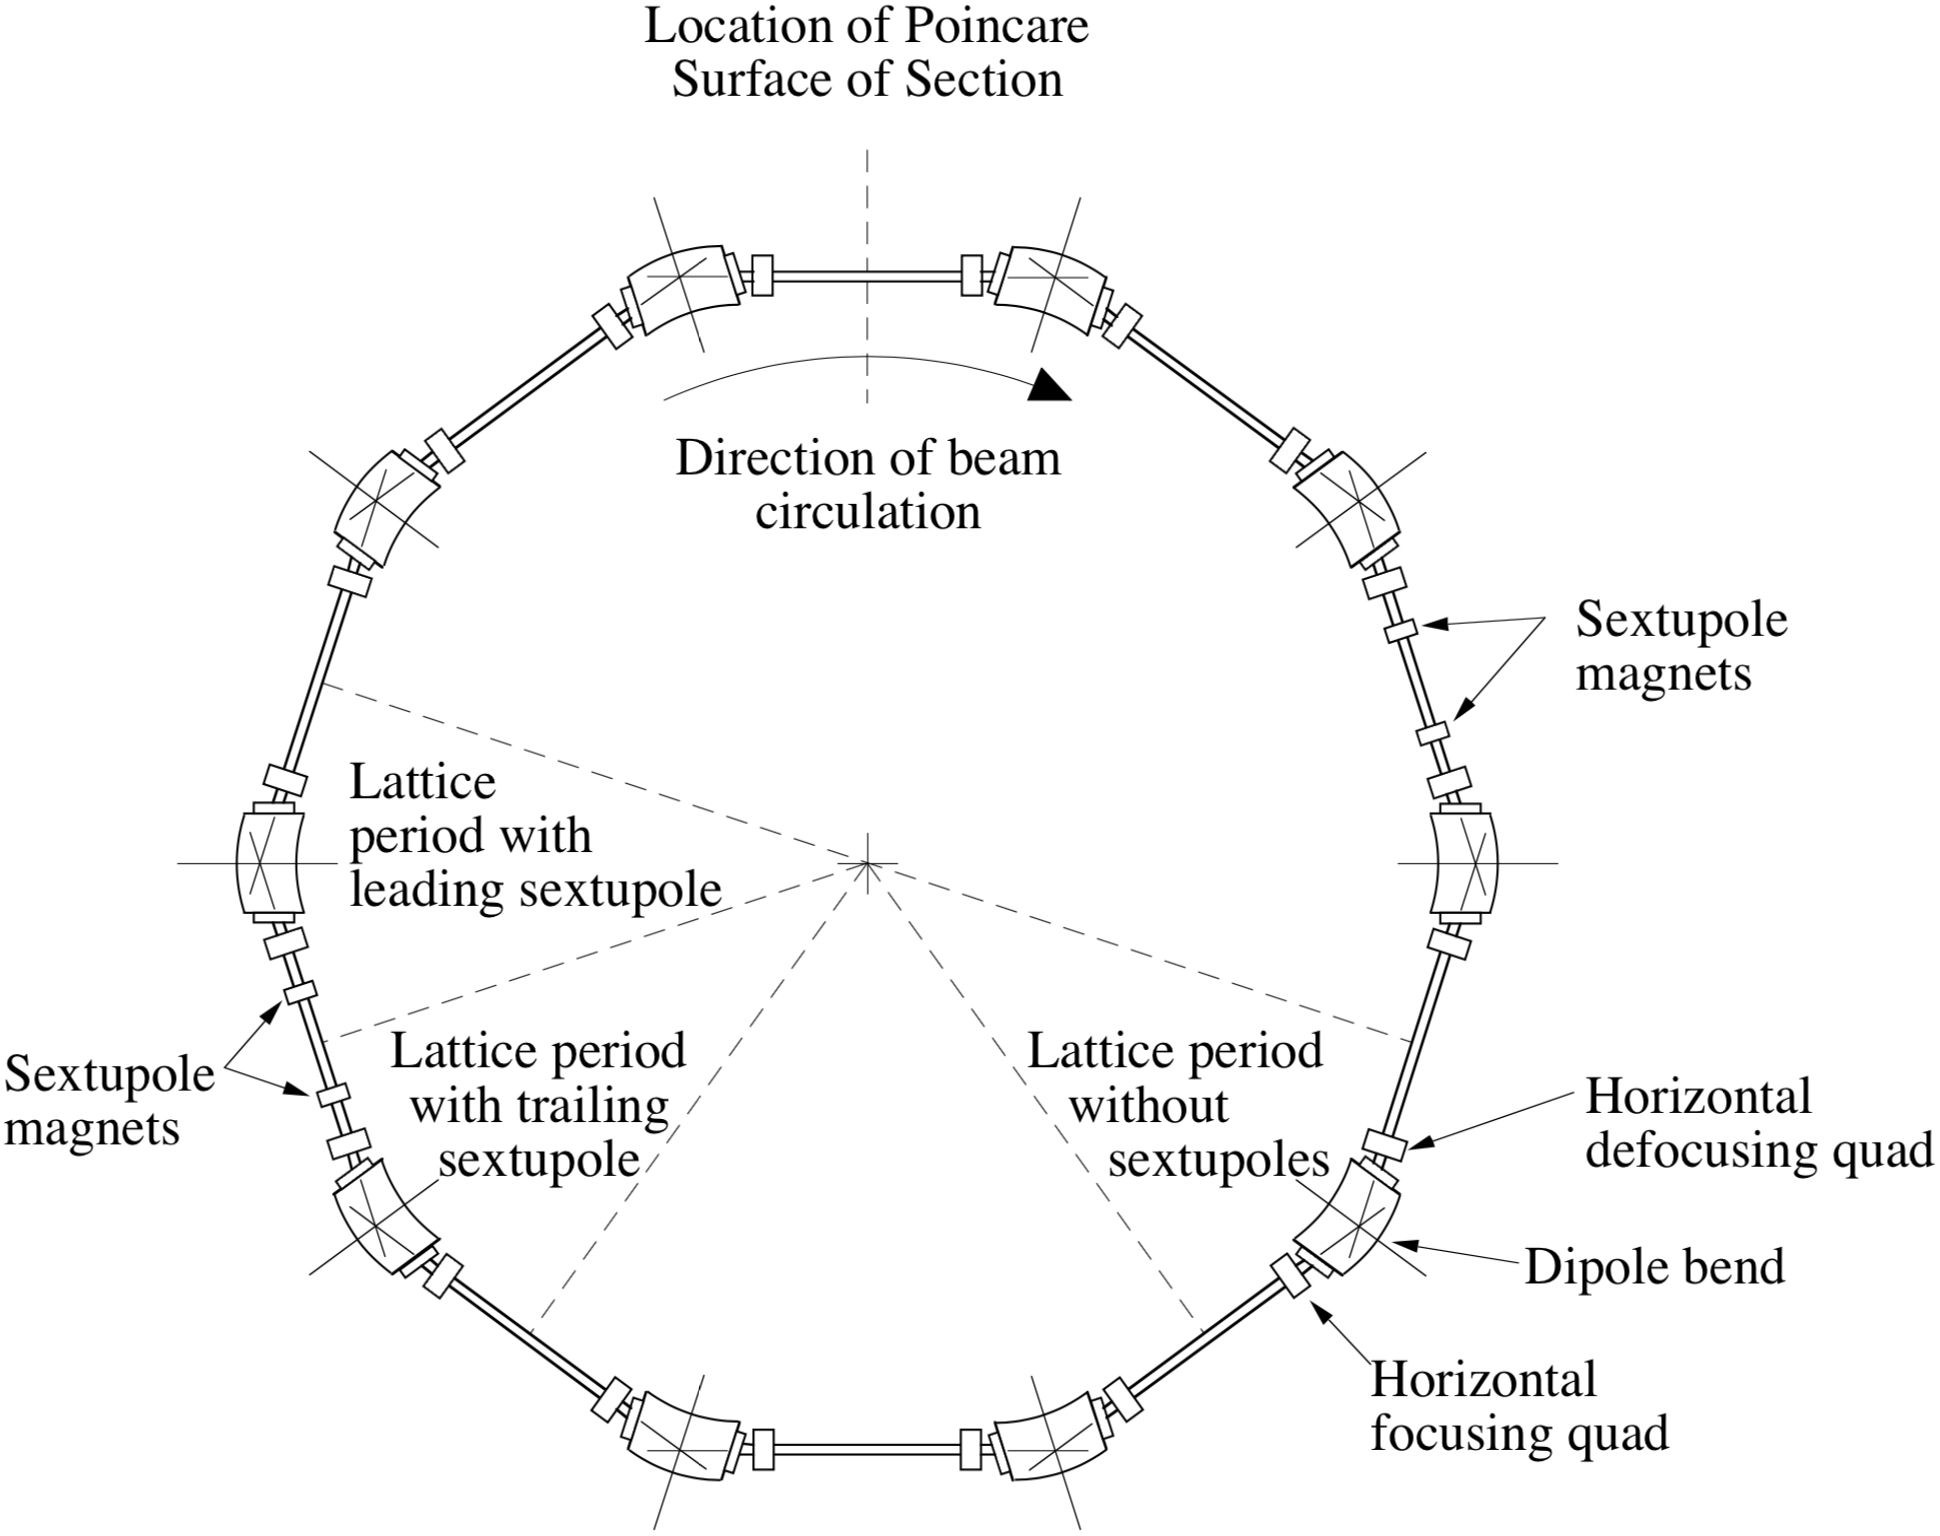
\includegraphics[scale=0.453]{ProtonLayout}
  \caption{Layout of Proton Storage Ring.}
\end{figure}

     Further inspection of the lattice shows that it can be viewed as being
composed of three kinds of periods.  These periods and their contents are
shown in figure 2.5.2.

\begin{figure}[htb]
  \centering
  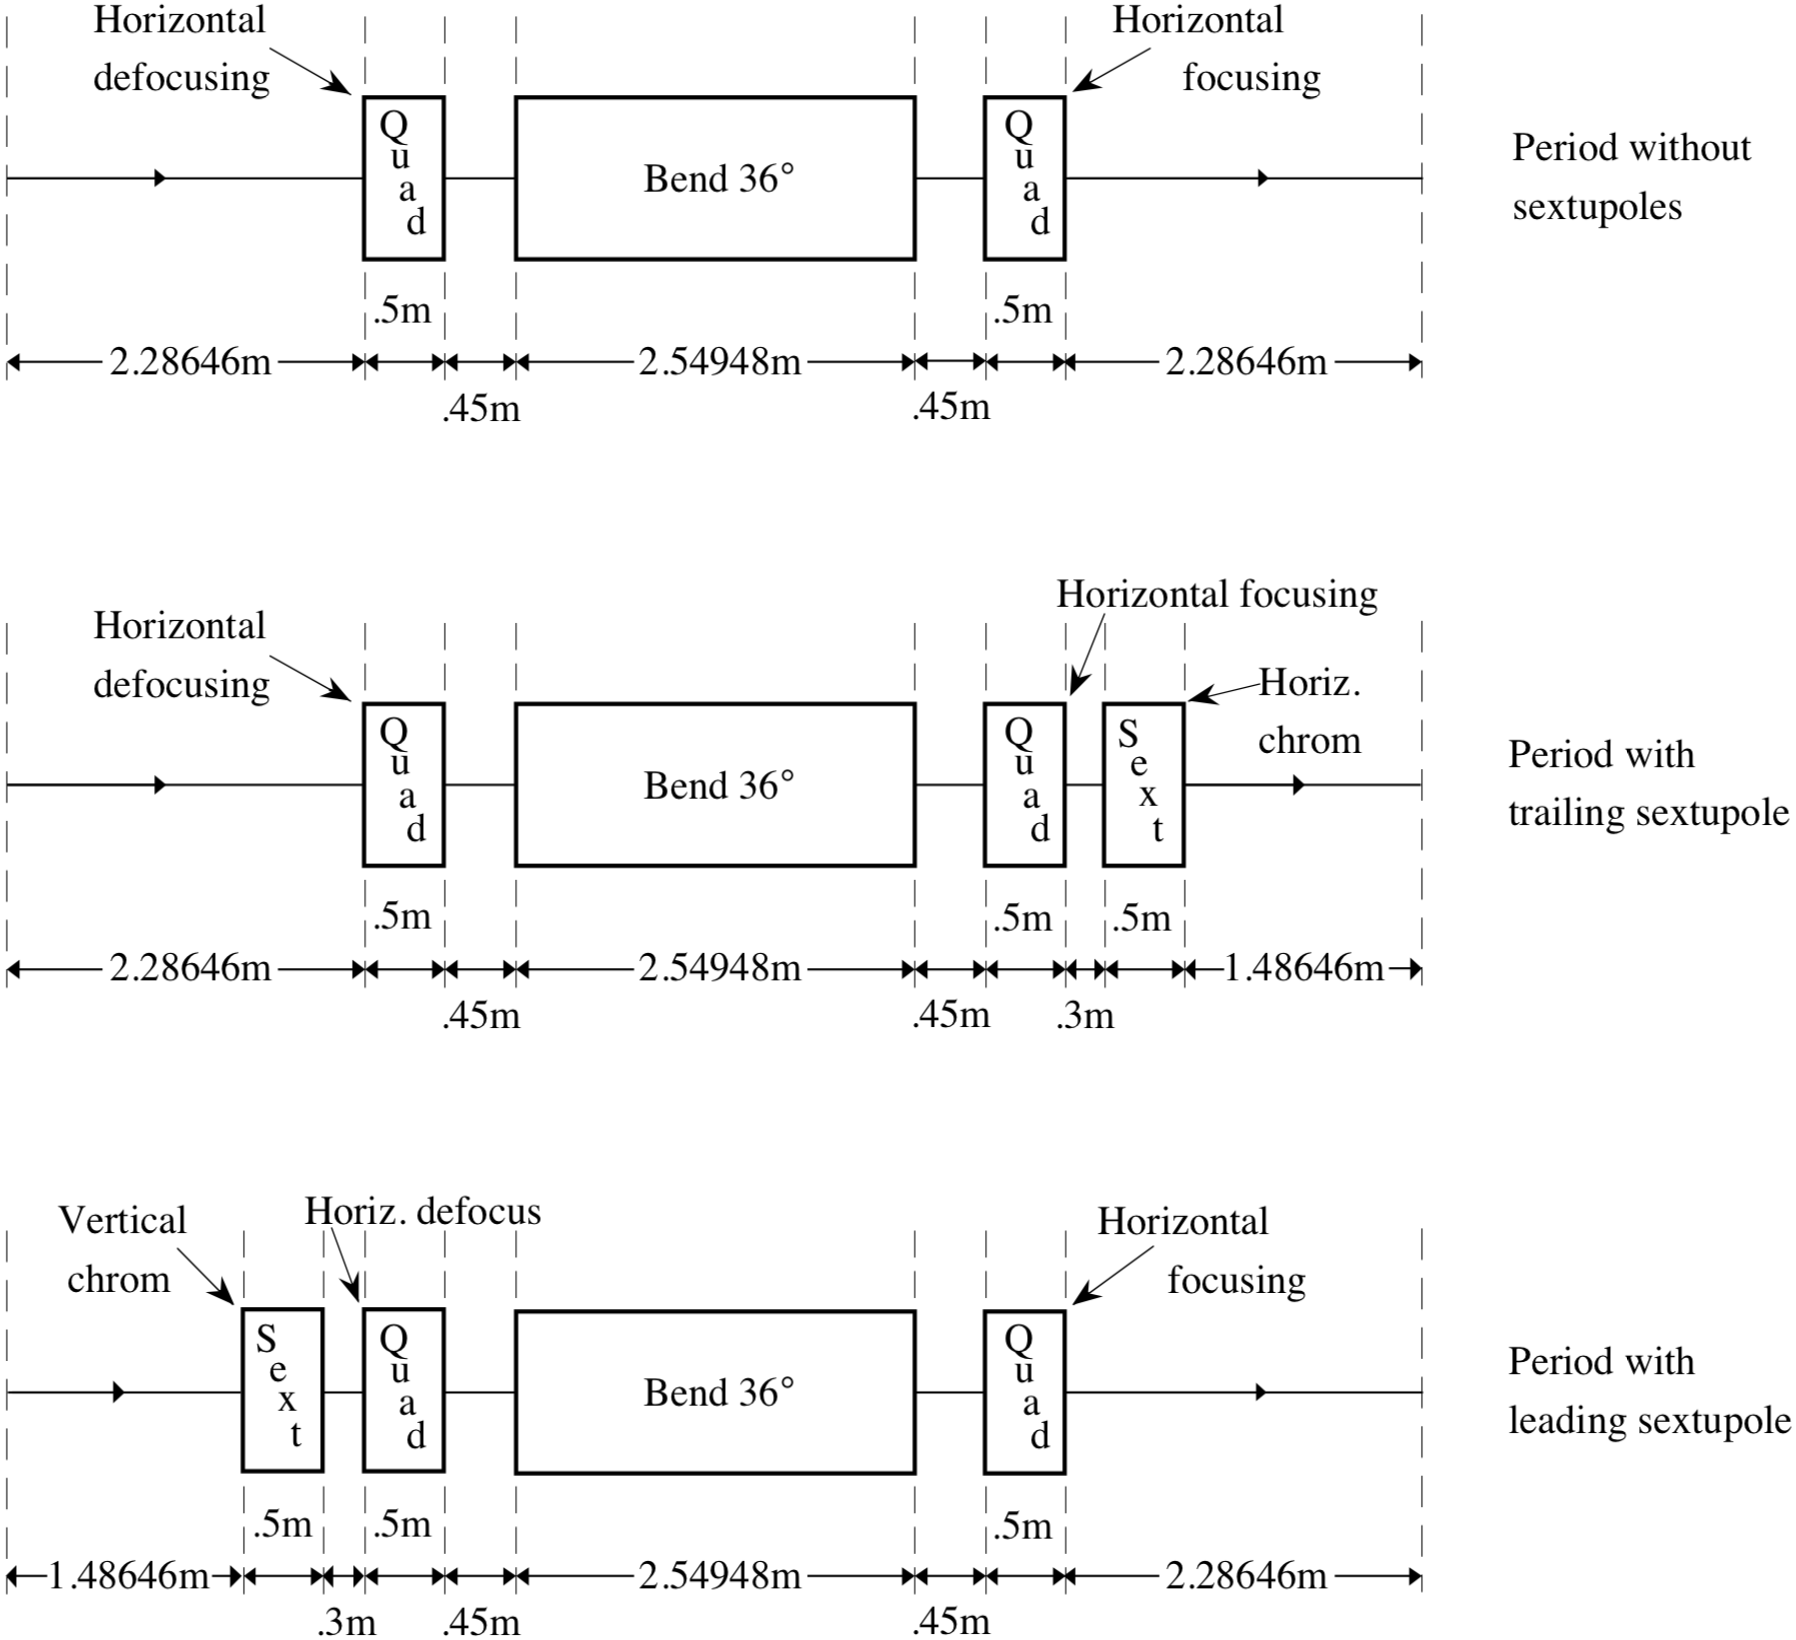
\includegraphics[scale=0.453]{ProtonRing}
  \caption{Details and dimensions of constituent
                       periods of Proton Storage Ring.}
\end{figure}


     To analyze the performance of the proton storage ring, it is useful to
make two sets of \Mary runs.  The first set of runs will be made to study
the one-turn transfer map for the ring.  The second set will examine
long-term orbit behavior.

     The results of a preliminary run to study the one-turn transfer map
are shown below:

{
\footnotesize\tt
\begin{verbatim}

#comment
 Exhibit 2.5.1
 This is a study of a small static storage ring.
 This MARYLIE run will analyze the one lattice period
 and one turn transfer maps.
#beam
  4.86914813175970
 0.849425847892200
  1.00000000000000
  1.00000000000000
#menu
 drvs     drft
  0.300000000000000
 drs      drft
  0.450000000000000
 drml     drft
   1.48646000000000
 drl      drft
   2.28646000000000
 bend     pbnd
   36.0000000000000      0.000000000000000E+00  0.500000000000000
   1.20000000000000
 hfq      quad
  0.500000000000000       2.72000000000000      0.000000000000000E+00
  0.000000000000000E+00
 hdq      quad
  0.500000000000000      -1.92000000000000      0.000000000000000E+00
  0.000000000000000E+00
 hcs      sext
  0.500000000000000      0.000000000000000E+00
 vcs      sext
  0.500000000000000      0.000000000000000E+00
 fileout  pmif
   1.00000000000000       12.0000000000000       3.00000000000000
 mapout   ptm
   3.00000000000000       3.00000000000000      0.000000000000000E+00
  0.000000000000000E+00   1.00000000000000
 raysin   rt
   13.0000000000000       14.0000000000000      -1.00000000000000
  0.000000000000000E+00  0.000000000000000E+00  0.000000000000000E+00
 track    rt
   13.0000000000000       14.0000000000000       5.00000000000000
   500.000000000000       1.00000000000000      0.000000000000000E+00
 chrom    tasm
   2.00000000000000      1.000000000000000E-03   1.00000000000000
  0.000000000000000E+00   3.00000000000000      0.000000000000000E+00
 iden     iden
 fin      end
#lines
 nsex
     1*drl         1*hdq         1*drs         1*bend        1*drs      &
     1*hfq         1*drl
 tsex
     1*drl         1*hdq         1*drs         1*bend        1*drs      &
     1*hfq         1*drvs        1*hcs         1*drml
 lsex
     1*drml        1*vcs         1*drvs        1*hdq         1*drs      &
     1*bend        1*drs         1*hfq         1*drl
 half
     1*nsex        1*tsex        1*lsex        1*nsex        1*nsex
 ring
     2*half
#lumps
#loops
#labor
    1*fileout
    1*nsex
    1*chrom
    1*iden
    1*ring
    1*chrom
    1*mapout
    1*fin

twiss analysis of static map

tunes and chromaticities for delta defined in terms of momentum deviation:

horizontal tune =  0.225410281174760
first order horizontal chromaticity = -9.281703934545682E-002
second order horizontal chromaticity =  0.104559371148683
horizontal tune when delta =  1.000000000000000E-003
 0.225317568694785

vertical tune =  0.225543770585176
first order vertical chromaticity = -0.211132387676014
second order vertical chromaticity =  0.252919932812798
vertical tune when delta =  1.000000000000000E-003
 0.225332891117433

tune separation when delta=  1.000000000000000E-003
-1.532242264759565E-005

normalized anharmonicities
 hhn=  7.695357766309113E-003
 vvn=  1.802675106441745E-002
 hvn=  2.675634626130963E-002

twiss analysis of static map

tunes and chromaticities for delta defined in terms of momentum deviation:

horizontal tune =  0.254102811747596
first order horizontal chromaticity = -0.928170393454570
second order horizontal chromaticity =   1.04559371148684
horizontal tune when delta =  1.000000000000000E-003
 0.253175686947853

vertical tune =  0.255437705851761
first order vertical chromaticity =  -2.11132387676014
second order vertical chromaticity =   2.52919932812798
vertical tune when delta =  1.000000000000000E-003
 0.253328911174329

tune separation when delta=  1.000000000000000E-003
-1.532242264760675E-004

normalized anharmonicities
 hhn=  7.695357766309278E-002
 vvn=  0.180267510644177
 hvn=  0.267563462613096

matrix for map is :

 8.79899E-01  6.43546E+00  0.00000E+00  0.00000E+00  0.00000E+00 -3.09884E+00
-2.82743E-01 -9.31451E-01  0.00000E+00  0.00000E+00  0.00000E+00 -3.07914E-01
 0.00000E+00  0.00000E+00 -9.04734E-01  6.22828E+00  0.00000E+00  0.00000E+00
 0.00000E+00  0.00000E+00 -2.82058E-01  8.36415E-01  0.00000E+00  0.00000E+00
 1.14711E+00  4.86799E+00  0.00000E+00  0.00000E+00  1.00000E+00  1.30681E+01
 0.00000E+00  0.00000E+00  0.00000E+00  0.00000E+00  0.00000E+00  1.00000E+00

nonzero elements in generating polynomial are :

 f( 28)=f( 30 00 00 )=-1.14530840551473E-02
 f( 29)=f( 21 00 00 )= 2.67517165681652E-02
 f( 33)=f( 20 00 01 )= -1.1736777355489
 f( 34)=f( 12 00 00 )= 8.77407347896805E-04
 f( 38)=f( 11 00 01 )= -6.7730221731743
 f( 39)=f( 10 20 00 )=-6.01680421031948E-02
 f( 40)=f( 10 11 00 )= 0.67669439436590
 f( 43)=f( 10 02 00 )= -1.8306262274435
 f( 48)=f( 10 00 02 )= -6.0154921926825
 f( 49)=f( 03 00 00 )= 0.16593635071889
 f( 53)=f( 02 00 01 )= -23.642071165236
 f( 54)=f( 01 20 00 )=-3.44440710710079E-02
 f( 55)=f( 01 11 00 )= 3.85161039824409E-02
 f( 58)=f( 01 02 00 )=  1.4627612575911
 f( 63)=f( 01 00 02 )= -8.7202857803725
 f( 67)=f( 00 20 01 )= -2.4822497040586
 f( 70)=f( 00 11 01 )=  16.699387190479
 f( 76)=f( 00 02 01 )= -57.101990751187
 f( 83)=f( 00 00 03 )= -34.310069304168
 f( 84)=f( 40 00 00 )=-1.37013931670580E-02
 f( 85)=f( 31 00 00 )=-0.16784866108730
 f( 89)=f( 30 00 01 )=-0.31703479901659
 f( 90)=f( 22 00 00 )=-0.92855072951694
 f( 94)=f( 21 00 01 )= -2.9203989725275
 f( 95)=f( 20 20 00 )=-0.12024362379291
 f( 96)=f( 20 11 00 )= 0.62813570271803
 f( 99)=f( 20 02 00 )= -1.3387286297467
 f(104)=f( 20 00 02 )= -3.4667565555761
 f(105)=f( 13 00 00 )= -2.6538649658506
 f(109)=f( 12 00 01 )= -8.5904681059051
 f(110)=f( 11 20 00 )=-0.57379494301836
 f(111)=f( 11 11 00 )=  2.4415653749948
 f(114)=f( 11 02 00 )= -6.2836394557255
 f(119)=f( 11 00 02 )= -22.589602187849
 f(123)=f( 10 20 01 )= -1.5269177137599
 f(126)=f( 10 11 01 )=  8.6399711664208
 f(132)=f( 10 02 01 )= -9.5208000216435
 f(139)=f( 10 00 03 )= -13.291152725777
 f(140)=f( 04 00 00 )= -4.9592065206488
 f(144)=f( 03 00 01 )=  1.9246183284199
 f(145)=f( 02 20 00 )= -1.2337505894646
 f(146)=f( 02 11 00 )=  7.7049990878473
 f(149)=f( 02 02 00 )= -34.462207995042
 f(154)=f( 02 00 02 )= -63.008955902638
 f(158)=f( 01 20 01 )= -5.3711963846800
 f(161)=f( 01 11 01 )=  23.661202919812
 f(167)=f( 01 02 01 )=  36.336091551217
 f(174)=f( 01 00 03 )= -27.562892961455
 f(175)=f( 00 40 00 )=-2.57477900501080E-02
 f(176)=f( 00 31 00 )= 0.32207137603156
 f(179)=f( 00 22 00 )= -1.9603982221369
 f(184)=f( 00 20 02 )= -6.2193628931016
 f(185)=f( 00 13 00 )=  6.2167715680490
 f(190)=f( 00 11 02 )=  40.018453416659
 f(195)=f( 00 04 00 )= -11.878247622830
 f(200)=f( 00 02 02 )= -117.09988758729
 f(209)=f( 00 00 04 )= -51.586059604493

\end{verbatim}}

     The reader is invited to compare the contents of the lines {\em nsex}, {\em tsex},
and {\em lsex} with the contents of the three periods shown in figure 2.5.2.  He
or she should also compare the contents of the lines {\em half } and {\em ring } with the
contents of the lattice as shown in figure 2.5.1.  Next, the reader should
note that although 0.5 meter sextupoles occur in {\em \#menu} under the user names
{\em hcs } and {\em vcs}, the second parameter for each sextupole (which specifies the
sextupole strength) has been set equal to zero.  Finally, the reader should
observe that the fringe fields for all the quadrupoles have been ``turned
off'' since the last two parameters associated with each quadrupole are both
zero.

     Some entries in the {\em \#labor} component of the Master Input File also
call for comment.  The entry {\em nsex } calls for the computation of the transfer
map described by the line {\em nsex } (corresponding to a lattice period with no
sextupoles).  The command {\em chrom } then calls for the computation of the
tunes, chromaticities, and anharmonicities (tune dependence on betatron
amplitude).  Next, the transfer map is reset to the identity map by means
of the command {\em iden}.

     Subsequently, the entry {\em ring } and the (repeated) command {\em chrom } call
respectively for the computation of the transfer map for the full ring and
the computation of its tunes, chromaticities, etc.  Finally, {\em mapout } calls
for the printing out of the transfer map for the full ring, i.e., the
one-turn transfer map.

     To see what results from these entries and commands, look at the two
blocks of output that follow the {\em \#labor} component.  The reader should find
a listing of the tune, first-order chromaticity, and second-order
chromaticity for both the horizontal and vertical degrees of freedom.  The
first block of output gives this information for the transfer map
corresponding to a single lattice period, and the second block gives this
information for a full turn.

     Evidently, the horizontal and vertical tunes for a single lattice
period are $.2254\ldots$ and $.2255\ldots$, respectively.  Correspondingly, the
first-order horizontal and vertical chromaticities are $-.092\ldots$ and $-.211\ldots$, respectively.

     Since the full ring is composed of ten periods, one would expect the
tunes and chromaticities for the full ring (given in the second block of
output) to be 10 times as large as those for a single lattice period.
This is indeed the case.  However, because \Mary computes tunes directly
from the total transfer map, it gives only the fractional (and not the
integer) parts of tunes.  Thus, the horizontal and vertical tunes for one
full turn are $2.254\ldots$ and $2.255\ldots$, and \Mary gives the values $.254\ldots$
and $.255\ldots$, respectively.  See sections 8.2 and 10.10.

     Finally, it should be observed that since the sextupoles are off for
this particular \Mary run, the chromaticities computed are the natural
chromaticities of the ring.  Correspondingly, the ring is composed entirely
of what are normally regarded as linear elements.  However, inspection of
the generating polynomial for the nonlinear part of the one-turn transfer
map shows that there are, in fact, a large number of nonzero elements.
Thus, as should have already been obvious from the previous examples of
single pass systems, even the so-called linear elements have nonlinear
effects.

     Suppose it is desired to run the Proton Storage Ring in a mode for
which the design orbit has no first-order chromaticities.  This can be
accomplished by giving the sextupoles suitable nonzero strengths.  Shown
below is a \Mary run for this case:

{
\footnotesize\tt
\begin{verbatim}
 #comment
  Exhibit 2.5.2.
  This is a study of a small static storage ring.
  This MARYLIE run will analyze the one turn transfer map when
  chromaticity correcting sextupoles are turned on.
  The effect of hard-edge quadrupole fringe fields is also included.
 #beam
   4.869148131759700
   0.8494258478922000
   1.000000000000000
   1.000000000000000
 #menu
  drvs     drft
   0.300000000000000
  drs      drft
   0.450000000000000
  drml     drft
    1.48646000000000
  drl      drft
    2.28646000000000
  bend     pbnd
    36.0000000000000      0.000000000000000E+00  0.500000000000000
    1.20000000000000
  hfq      quad
   0.500000000000000       2.72000000000000       1.00000000000000
    1.00000000000000
  hdq      quad
   0.500000000000000      -1.92000000000000       1.00000000000000
    1.00000000000000
  hcs      sext
   0.500000000000000       1.62000000000000
  vcs      sext
   0.500000000000000      -3.34000000000000
  fileout  pmif
    1.00000000000000       12.0000000000000       3.00000000000000
  mapout   ptm
    3.00000000000000       3.00000000000000      0.000000000000000E+00
   0.000000000000000E+00   1.00000000000000
  raysin   rt
    13.0000000000000       14.0000000000000      -1.00000000000000
   0.000000000000000E+00  0.000000000000000E+00  0.000000000000000E+00
  track    rt
    13.0000000000000       14.0000000000000       5.00000000000000
    500.000000000000       1.00000000000000      0.000000000000000E+00
  chrom    tasm
    2.00000000000000      1.000000000000000E-03   1.00000000000000
   0.000000000000000E+00   3.00000000000000      0.000000000000000E+00
  iden     iden
  fin      end
 #lines
  nsex
      1*drl       1*hdq         1*drs         1*bend        1*drs   &
      1*hfq       1*drl
  tsex
      1*drl       1*hdq         1*drs         1*bend        1*drs   &
      1*hfq       1*drvs        1*hcs         1*drml
  lsex
      1*drml      1*vcs         1*drvs        1*hdq         1*drs   &
      1*bend      1*drs         1*hfq         1*drl
  half
      1*nsex      1*tsex        1*lsex        1*nsex        1*nsex
  ring
      2*half
 #lumps
 #loops
 #labor
     1*fileout
     1*ring
     1*chrom
     1*mapout
     1*fin

 twiss analysis of static map

 tunes and chromaticities for delta defined in terms of momentum deviation
 horizontal tune =  0.2541028117475962
 first order horizontal chromaticity = -2.9470801637403564E-04
 second order horizontal chromaticity =   48.16025275066844
 horizontal tune when delta =  9.9999999999999999E-04
  0.2541506772923305

 vertical tune =  0.2554377058517620
 first order vertical chromaticity =  2.5713854609451646E-03
 second order vertical chromaticity =   5.969652580601808
 vertical tune when delta =  9.9999999999999999E-04
  0.2554462468898036

 tune separation when delta=  9.9999999999999999E-04
 -1.2955695974730605E-03

 normalized anharmonicities
  hhn=   4.463887843064638
  vvn=  -1.491178186878906
  hvn= -0.1610999831430029

 matrix for map is :

 8.79899E-01  6.43546E+00  0.00000E+00 0.00000E+00 0.00000E+00 -3.09884E+00
-2.82743E-01 -9.31451E-01  0.00000E+00 0.00000E+00 0.00000E+00 -3.07914E-01
 0.00000E+00  0.00000E+00 -9.04734E-01 6.22828E+00 0.00000E+00  0.00000E+00
 0.00000E+00  0.00000E+00 -2.82058E-01 8.36415E-01 0.00000E+00  0.00000E+00
 1.14711E+00  4.86799E+00  0.00000E+00 0.00000E+00 1.00000E+00  1.30681E+01
 0.00000E+00  0.00000E+00  0.00000E+00 0.00000E+00 0.00000E+00  1.00000E+00

 nonzero elements in generating polynomial are :

  f( 28)=f( 30 00 00 )=-0.24592784728790D+00
  f( 29)=f( 21 00 00 )=-0.30604852898231D+01
  f( 33)=f( 20 00 01 )=-0.64563088742748D+00
  f( 34)=f( 12 00 00 )=-0.15583145022099D+02
  f( 38)=f( 11 00 01 )= 0.18502158940524D+01
  f( 39)=f( 10 20 00 )=-0.12483369572898D+00
  f( 40)=f( 10 11 00 )= 0.27148128836245D+01
  f( 43)=f( 10 02 00 )=-0.87122374564362D+01
  f( 48)=f( 10 00 02 )=-0.84099767967792D+01
  f( 49)=f( 03 00 00 )=-0.25619634656306D+02
  f( 53)=f( 02 00 01 )=-0.98753574315669D+01
  f( 54)=f( 01 20 00 )=-0.41957680678127D+01
  f( 55)=f( 01 11 00 )= 0.41001609885339D+02
  f( 58)=f( 01 02 00 )=-0.10461799484601D+03
  f( 63)=f( 01 00 02 )= 0.12493092450878D+01
  f( 67)=f( 00 20 01 )= 0.24840176792545D+01
  f( 70)=f( 00 11 01 )=-0.24548154751239D+02
  f( 76)=f( 00 02 01 )= 0.37914232657814D+02
  f( 83)=f( 00 00 03 )=-0.43860487074368D+02
  f( 84)=f( 40 00 00 )=-0.53238969994112D+00
  f( 85)=f( 31 00 00 )=-0.52691073709927D+01
  f( 89)=f( 30 00 01 )=-0.76197059527104D+01
  f( 90)=f( 22 00 00 )=-0.33384606194653D+02
  f( 94)=f( 21 00 01 )=-0.45466953399356D+02
  f( 95)=f( 20 20 00 )= 0.30176483526703D+00
  f( 96)=f( 20 11 00 )=-0.73344825077518D+01
  f( 99)=f( 20 02 00 )= 0.48285862483518D+01
  f(104)=f( 20 00 02 )=-0.70911206118901D+02
  f(105)=f( 13 00 00 )=-0.13016712967035D+03
  f(109)=f( 12 00 01 )=-0.77668739786113D+02
  f(110)=f( 11 20 00 )= 0.10964795411111D+02
  f(111)=f( 11 11 00 )=-0.96814661908489D+02
  f(114)=f( 11 02 00 )= 0.67959248309980D+02
  f(119)=f( 11 00 02 )=-0.41584221544659D+03
  f(123)=f( 10 20 01 )=-0.71637764336681D+01
  f(126)=f( 10 11 01 )= 0.47588769596512D+02
  f(132)=f( 10 02 01 )=-0.19324624884052D+03
  f(139)=f( 10 00 03 )=-0.21947536145204D+03
  f(140)=f( 04 00 00 )=-0.33768147778230D+03
  f(144)=f( 03 00 01 )= 0.22187955157124D+03
  f(145)=f( 02 20 00 )= 0.26092739583358D+02
  f(146)=f( 02 11 00 )=-0.29953156756094D+03
  f(149)=f( 02 02 00 )= 0.33203293824300D+03
  f(154)=f( 02 00 02 )=-0.12804942840066D+04
  f(158)=f( 01 20 01 )=-0.33119338725585D+02
  f(161)=f( 01 11 01 )= 0.38145383287607D+03
  f(167)=f( 01 02 01 )=-0.13066261557003D+04
  f(174)=f( 01 00 03 )=-0.22257971295707D+03
  f(175)=f( 00 40 00 )= 0.21231457461353D+00
  f(176)=f( 00 31 00 )=-0.60270556962489D+01
  f(179)=f( 00 22 00 )= 0.43923145828609D+02
  f(184)=f( 00 20 02 )=-0.72981558046921D+01
  f(185)=f( 00 13 00 )=-0.12013612969892D+03
  f(190)=f( 00 11 02 )= 0.50696669600891D+02
  f(195)=f( 00 04 00 )= 0.43239694128681D+02
  f(200)=f( 00 02 02 )=-0.38530783430069D+03
  f(209)=f( 00 00 04 )=-0.44005157367639D+03
\end{verbatim}}


     Note that the first-order chromaticities are now inconsequential.
Also, the second-order chromaticities have changed.  This is partly due to
turning on the sextupoles, and partly due to the inclusion of hard-edge
quadrupole fringe field effects.  (Observe that the quadrupoles appearing
in {\em \#menu} now have their fringe fields turned on.)  Finally, the reader
should compare the nonlinear content of the transfer map (the generating
polynomial) for the two cases for which the sextupoles are turned off and
turned on.  As might be expected, the nonlinear content is much higher for
the case in which the sextupoles are turned on.

     It is well known that nonlinearities in the one-turn transfer map can
produce nonlinear structure resonances.  Below is a \Mary run
illustrating typical 1/3 integer resonance behavior.  The quadrupole
strengths have been adjusted to give a horizontal tune of approximately
1.33 for half a turn, and the sextupoles have been readjusted to again
achieve negligible first-order chromaticities.

{
\footnotesize\tt
\begin{verbatim}
 #comment
  Exhibit 2.5.3.
  This is a study of a small static storage ring.
  This MARYLIE run will analyze the half turn transfer map, and then
  track multiple half turns through the lattice.
 #beam
   4.869148131759700
  0.8494258478922000
   1.000000000000000
   1.000000000000000
 #menu
  drvs     drft
   0.300000000000000
  drs      drft
   0.450000000000000
  drml     drft
    1.48646000000000
  drl      drft
    2.28646000000000
  bend     pbnd
    36.0000000000000      0.000000000000000E+00  0.500000000000000
    1.20000000000000
  hfq      quad
   0.500000000000000       3.13000000000000       1.00000000000000
    1.00000000000000
  hdq      quad
   0.500000000000000      -1.92000000000000       1.00000000000000
    1.00000000000000
  hcs      sext
   0.500000000000000       2.65000000000000
  vcs      sext
   0.500000000000000      -5.01000000000000
  fileout  pmif
    1.00000000000000       12.0000000000000       3.00000000000000
  mapout   ptm
    3.00000000000000       3.00000000000000      0.000000000000000E+00
   0.000000000000000E+00   1.00000000000000
  raysin   rt
    13.0000000000000       14.0000000000000      0.00000000000000
   0.000000000000000E+00  0.000000000000000E+00  0.000000000000000E+00
  track    rt
   0.000000000000000E+00   14.0000000000000       5.00000000000000
    310.000000000000       1.00000000000000      0.000000000000000E+00
  chrom    tasm
    2.00000000000000      1.000000000000000E-03   1.00000000000000
   0.000000000000000E+00   3.00000000000000      0.000000000000000E+00
  iden     iden
  fin      end
 #lines
  nsex
      1*drl      1*hdq         1*drs         1*bend        1*drs    &
      1*hfq      1*drl
  tsex
      1*drl      1*hdq         1*drs         1*bend        1*drs    &
      1*hfq      1*drvs        1*hcs         1*drml
  lsex
      1*drml     1*vcs         1*drvs        1*hdq         1*drs    &
      1*bend     1*drs         1*hfq         1*drl
  half
      1*nsex     1*tsex        1*lsex        1*nsex        1*nsex
  ring
      2*half
 #lumps
 #loops
 #labor
     1*fileout
     1*iden
     1*raysin
     1*half
     1*chrom
     1*mapout
     1*track
     1*fin

 twiss analysis of static map

 tunes and chromaticities for delta defined in terms of momentum deviation
 horizontal tune =  0.3301854790746201
 first order horizontal chromaticity = -5.0836441463590513E-04
 second order horizontal chromaticity =   32.78527399985234
 horizontal tune when delta =  9.9999999999999999E-04
  0.3302177559842053

 vertical tune =  6.3227244365018311E-02
 first order vertical chromaticity = -8.9058574997704199E-04
 second order vertical chromaticity =  -24.35635555300784
 vertical tune when delta =  9.9999999999999999E-04
  6.3201997423715326E-02

 tune separation when delta=  9.9999999999999999E-04
  0.2670157585604900

 normalized anharmonicities
  hhn=   38.34696150586799
  vvn=  0.6125175935029140
  hvn=   2.867346907397344



 matrix for map is :

 3.71731E-01  4.86128E+00  0.00000E+00 0.00000E+00 0.00000E+00 -3.49162E+00
-3.07966E-01 -1.33728E+00  0.00000E+00 0.00000E+00 0.00000E+00 -1.01272E-01
 0.00000E+00  0.00000E+00  5.48139E-01 2.60973E+00 0.00000E+00  0.00000E+00
 0.00000E+00  0.00000E+00 -1.10952E-01 1.29610E+00 0.00000E+00  0.00000E+00
 1.11295E+00  5.16158E+00  0.00000E+00 0.00000E+00 1.00000E+00  1.05182E+01
 0.00000E+00  0.00000E+00  0.00000E+00 0.00000E+00 0.00000E+00  1.00000E+00

 nonzero elements in generating polynomial are :

  f( 28)=f( 30 00 00 )=-0.51714051077699D+00
  f( 29)=f( 21 00 00 )=-0.48790573879345D+01
  f( 33)=f( 20 00 01 )=-0.12713167778801D+01
  f( 34)=f( 12 00 00 )=-0.14356813797105D+02
  f( 38)=f( 11 00 01 )=-0.86091649476806D+01
  f( 39)=f( 10 20 00 )=-0.57480702313803D+00
  f( 40)=f( 10 11 00 )= 0.21535856911966D+01
  f( 43)=f( 10 02 00 )=-0.23385635802931D+00
  f( 48)=f( 10 00 02 )=-0.37903489409162D+01
  f( 49)=f( 03 00 00 )=-0.10095440524513D+02
  f( 53)=f( 02 00 01 )=-0.28749629612880D+02
  f( 54)=f( 01 20 00 )=-0.48676979484183D+01
  f( 55)=f( 01 11 00 )= 0.25178527593201D+02
  f( 58)=f( 01 02 00 )=-0.24955355122107D+02
  f( 63)=f( 01 00 02 )= 0.24870572685000D+00
  f( 67)=f( 00 20 01 )= 0.14190256085394D+01
  f( 70)=f( 00 11 01 )=-0.62848065640486D+01
  f( 76)=f( 00 02 01 )=-0.12548412723025D+02
  f( 83)=f( 00 00 03 )=-0.19367900524518D+02
  f( 84)=f( 40 00 00 )=-0.11226234932478D+01
  f( 85)=f( 31 00 00 )=-0.18508072322998D+02
  f( 89)=f( 30 00 01 )=-0.32033394382143D+01
  f( 90)=f( 22 00 00 )=-0.11657515022811D+03
  f( 94)=f( 21 00 01 )=-0.27687744938574D+02
  f( 95)=f( 20 20 00 )= 0.36539976777681D+00
  f( 96)=f( 20 11 00 )= 0.29849078410504D+01
  f( 99)=f( 20 02 00 )=-0.33854616670401D+02
  f(104)=f( 20 00 02 )=-0.28225116719140D+02
  f(105)=f( 13 00 00 )=-0.30562227805297D+03
  f(109)=f( 12 00 01 )=-0.10141517819812D+03
  f(110)=f( 11 20 00 )=-0.14302896201977D+01
  f(111)=f( 11 11 00 )= 0.32788559634194D+02
  f(114)=f( 11 02 00 )=-0.23241803238853D+03
  f(119)=f( 11 00 02 )=-0.17486265747802D+03
  f(123)=f( 10 20 01 )= 0.23607064778068D+01
  f(126)=f( 10 11 01 )=-0.47863190256744D+01
  f(132)=f( 10 02 01 )=-0.55908627470362D+02
  f(139)=f( 10 00 03 )=-0.62274396302562D+02
  f(140)=f( 04 00 00 )=-0.33795772995004D+03
  f(144)=f( 03 00 01 )=-0.55322509665632D+02
  f(145)=f( 02 20 00 )=-0.10918051207894D+02
  f(146)=f( 02 11 00 )= 0.31345401800685D+02
  f(149)=f( 02 02 00 )=-0.32070340565228D+03
  f(154)=f( 02 00 02 )=-0.46674394906494D+03
  f(158)=f( 01 20 01 )= 0.42047841022217D+01
  f(161)=f( 01 11 01 )= 0.55497877942788D+02
  f(167)=f( 01 02 01 )=-0.37957949141255D+03
  f(174)=f( 01 00 03 )=-0.95542857277093D+02
  f(175)=f( 00 40 00 )=-0.71081436705546D+00
  f(176)=f( 00 31 00 )= 0.13608837848327D+02
  f(179)=f( 00 22 00 )=-0.87030851323349D+02
  f(184)=f( 00 20 02 )=-0.51342116123916D+01
  f(185)=f( 00 13 00 )= 0.22956951922200D+03
  f(190)=f( 00 11 02 )= 0.32330038339298D+02
  f(195)=f( 00 04 00 )=-0.24720909402934D+03
  f(200)=f( 00 02 02 )=-0.16804924009243D+03
  f(209)=f( 00 00 04 )=-0.96401192952643D+02
\end{verbatim}}

Observe that the fractional part of the horizontal tune for the
half-turn transfer map is $.330\ldots$, and that the first order chromaticities
are near zero.  Next, note from the listing of the generating polynomial
that the transfer map has noticeable nonlinear content.

     Comment should also be made about some of the entries in {\em \#labor}.
Since the command {\em raysin } follows the command {\em iden}, the ray trace produced by
{\em raysin } is performed using the identity map.  This is simply a convenient way
of making the initial conditions appear as the first few entries in the
final condition file.  Later, the entry {\em half } eventually followed by the
command {\em track } results in the tracking of multiple turns (half-turn by
half-turn) around the ring. Tracking results are recorded on the final
condition file after every half turn.  The first few lines of the final
condition file are shown below.  The first 3 lines reproduce the content of
the initial condition file (as a result of the command {\em rays\/}), and
subsequent lines show the result of repeatedly applying the half-turn
transfer map to these 3 initial conditions.
\vspace{5mm}

       First few lines of final condition file from tracking run
\begin{footnotesize}
\begin{tt}
\begin{tabbing}
-1.699\=89E-07 -4.012\=00E-04 -9.380\=35E-08 -5.491\=85E-05 9.898\=83E-06 0.000\= \kill
\>$X$ \>$P_x$ \>$Y$ \>$P_y$ \>$\tau$ \>$P_{\tau}$
\end{tabbing}
\end{tt}
\vspace{-5mm}
\begin{verbatim}
 0.10000E-01   0.00000E+00 0.00000E+00 0.00000E+00   0.00000E+00 0.00000E+00
 0.50000E-02   0.00000E+00 0.00000E+00 0.00000E+00   0.00000E+00 0.00000E+00
 0.25000E-02   0.00000E+00 0.00000E+00 0.00000E+00   0.00000E+00 0.00000E+00
 0.37290E-02  -0.31237E-02 0.00000E+00 0.00000E+00   0.11325E-01 0.00000E+00
 0.18633E-02  -0.15511E-02 0.00000E+00 0.00000E+00   0.56131E-02 0.00000E+00
 0.93072E-03  -0.77275E-03 0.00000E+00 0.00000E+00   0.27944E-02 0.00000E+00
-0.13783E-01   0.30100E-02 0.00000E+00 0.00000E+00  -0.50733E-03 0.00000E+00
-0.68445E-0    0.14956E-02 0.00000E+00 0.00000E+00  -0.28377E-03 0.00000E+00
-0.34099E-02   0.74557E-03 0.00000E+00 0.00000E+00  -0.14956E-03 0.00000E+00
\end{verbatim}
\end{footnotesize}

     Now look at figure 2.5.3 below.  It shows a composite of results from
several tracking runs.  The 3 closed curves in the figure result from
plotting the $X,P_x$  content of the final condition file from the tracking
run just shown and described.  The remaining unbounded curves come from
additional tracking runs.


\begin{figure}[hbp]
  \centering
  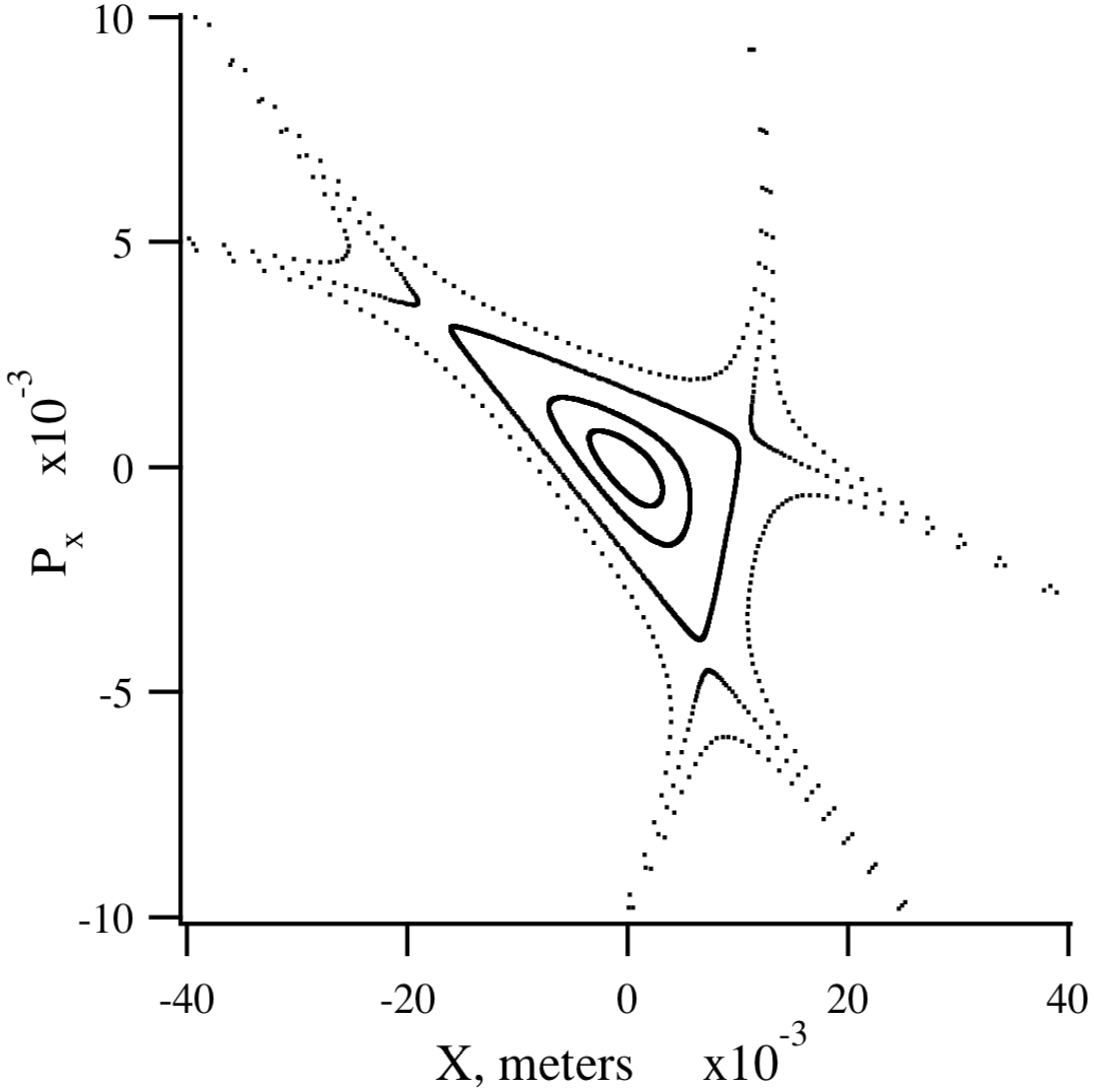
\includegraphics[height=3.5in]{psr3}
  \caption{ Horizontal phase-space plot illustrating
                  nonlinear instability when the horizontal
                      tune is near a 1/3 integer value.}
\end{figure}

     Evidently, as expected, nonlinearities in the one-turn transfer map
lead to instability if the betatron tune is near a 1/3 integer and the
betatron amplitude is too large.\index{nonlinear instability}  It is also easy to verify that this
effect is due to the chromaticity sextupoles.  To see this, one simply
makes another \Mary tracking run, for the same initial conditions, with
the sextupoles turned off.  Figure 2.5.4 below shows the result of making
and plotting such a run. Now all phase-space trajectories are stable in
that they appear to lie on smooth ellipses.


\begin{figure}[htp]
  \centering
  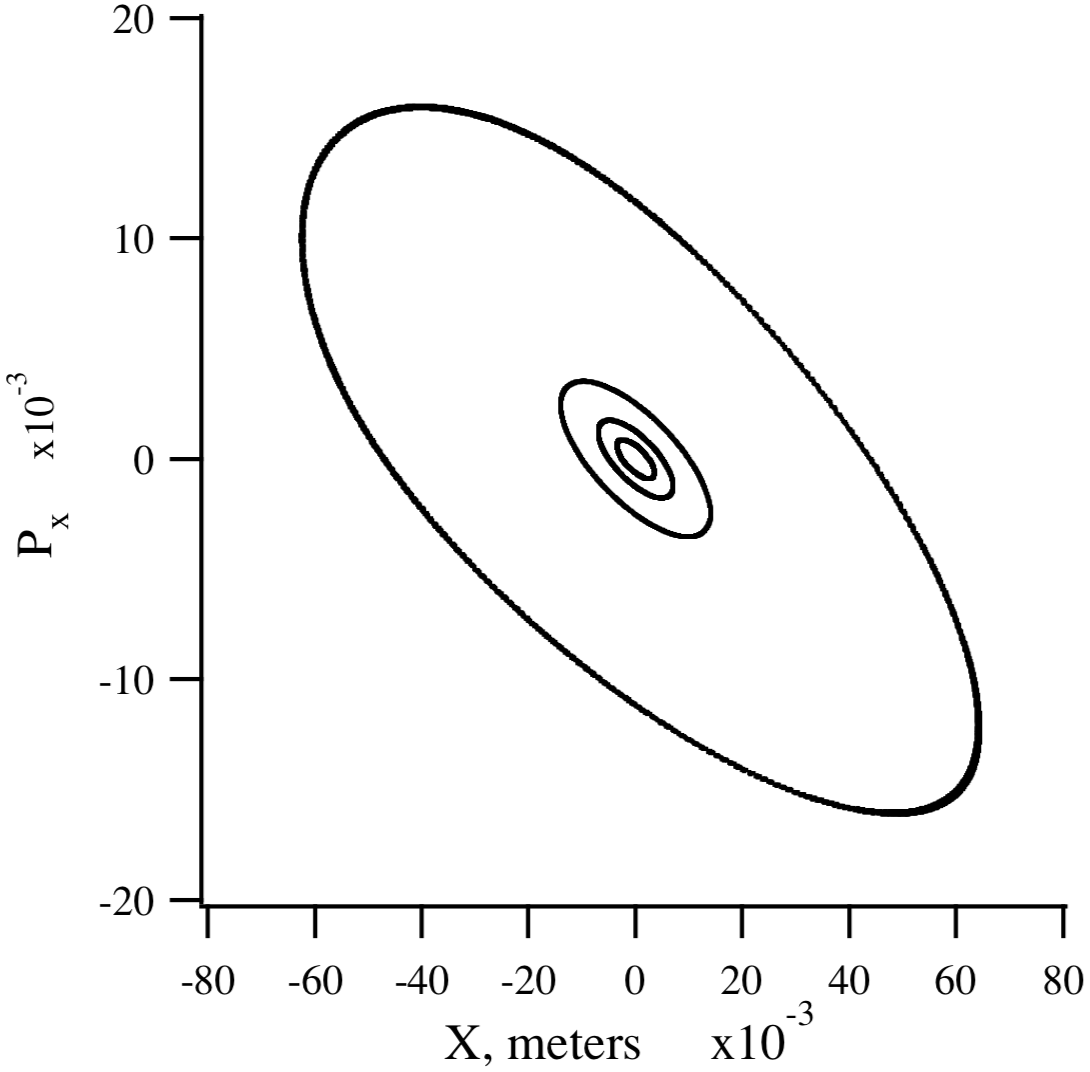
\includegraphics[height=3.5in]{psr3nosext}
  \caption{Horizontal phase-space plot made with the same
        initial conditions as figure 2.5.3 and sextupoles turned off.}
\end{figure}

     Nonlinearities in the one-turn transfer map can also have significant
effects on particle orbits even far away from resonant tunes.  Shown below
is an analysis and tracking run made for a case in which the quadrupoles
have been adjusted to give horizontal and vertical tunes of 3.254... and
2.253..., respectively, and the sextupoles have been reset to again achieve
very small first-order chromaticities.  Evidently, as can be seen from the
polynomial listing, the one-turn transfer map has noticeable nonlinear
content.

{
\footnotesize\tt
\begin{verbatim}
 #comment
  Exhibit 2.5.4.
  This is a study of a small static storage ring.
  Quad strengths are set to achieve horizontal and vertical tunes of
  approximately 3.25 and 2.25, respectively.
  Sextupole strengths are set to give negligible first order
  chromaticities.  This MARYLIE run will analyze the one turn transfer
  map and then track for 30,000 half turns.
 #beam
   4.869148131759700
  0.8494258478922000
   1.000000000000000
   1.000000000000000
 #menu
  drvs     drft
   0.300000000000000
  drs      drft
   0.450000000000000
  drml     drft
    1.48646000000000
  drl      drft
    2.28646000000000
  bend     pbnd
    36.0000000000000      0.000000000000000E+00  0.500000000000000
    1.20000000000000
  hfq      quad
   0.500000000000000       3.75000000000000       1.00000000000000
    1.00000000000000
  hdq      quad
   0.500000000000000      -2.20000000000000       1.00000000000000
    1.00000000000000
 hcs      sext
  0.500000000000000       4.18000000000000
 vcs      sext
  0.500000000000000      -7.84000000000000
 fileout  pmif
   1.00000000000000       12.0000000000000       3.00000000000000
 mapout   ptm
   3.00000000000000       3.00000000000000      0.000000000000000E+00
  0.000000000000000E+00   1.00000000000000
 raysin   rt
   13.0000000000000       14.0000000000000      -1.00000000000000
  0.000000000000000E+00  0.000000000000000E+00  0.000000000000000E+00
 track    rt
  0.000000000000000E+00   14.0000000000000       5.00000000000000
   30000.0000000000       3.00000000000000      0.000000000000000E+00
 chrom    tasm
   2.00000000000000      1.000000000000000E-03   1.00000000000000
  0.000000000000000E+00   3.00000000000000      0.000000000000000E+00
 iden     iden
 fin      end
#lines
 nsex
     1*drl         1*hdq         1*drs         1*bend        1*drs      &
     1*hfq         1*drl
 tsex
     1*drl         1*hdq         1*drs         1*bend        1*drs      &
     1*hfq         1*drvs        1*hcs         1*drml
 lsex
     1*drml        1*vcs         1*drvs        1*hdq         1*drs      &
     1*bend        1*drs         1*hfq         1*drl
 half
     1*nsex        1*tsex        1*lsex        1*nsex        1*nsex
 ring
     2*half
#lumps
#loops
#labor
    1*fileout
    1*raysin
    1*ring
    1*chrom
    1*mapout
    1*iden
    1*half
    1*track
    1*fin
    1 ray(s) read in from file  13

twiss analysis of static map
det in fxpt is     0.4198E+01

tunes and chromaticities for delta defined in terms of momentum deviation:

horizontal tune =  0.2547786892702122
first order horizontal chromaticity = -4.0271619374618478E-04
second order horizontal chromaticity =   32.65808774228796
horizontal tune when delta =  9.9999999999999999E-04
 0.2548109446417608

vertical tune =  0.2530051390161866
first order vertical chromaticity =  1.7975433225818153E-03
second order vertical chromaticity =  -22.15511182954404
vertical tune when delta =  9.9999999999999999E-04
 0.2529847814476796

tune separation when delta=  9.9999999999999999E-04
 1.8261631940811318E-03

normalized anharmonicities
 hhn=   53.24862334223061
 vvn=   26.85912432585413
 hvn=   30.24380891672483
det in fxpt is     0.4198E+01

matrix for map is :

 1.25112E+00  5.02535E+00  0.00000E+00  0.00000E+00  0.00000E+00 -9.78199E-01
-5.25419E-01 -1.31116E+00  0.00000E+00  0.00000E+00  0.00000E+00 -4.37925E-01
 0.00000E+00  0.00000E+00 -1.14286E+00  6.61944E+00  0.00000E+00  0.00000E+00
 0.00000E+00  0.00000E+00 -3.41867E-01  1.10510E+00  0.00000E+00  0.00000E+00
 1.06186E+00  3.48330E+00  0.00000E+00  0.00000E+00  1.00000E+00  2.51190E+01
 0.00000E+00  0.00000E+00  0.00000E+00  0.00000E+00  0.00000E+00  1.00000E+00

nonzero elements in generating polynomial are :

 f( 28)=f( 30 00 00 )= 0.19670225454821D+00
 f( 29)=f( 21 00 00 )= 0.55152652415966D+01
 f( 33)=f( 20 00 01 )=-0.52761919484391D+01
 f( 34)=f( 12 00 00 )= 0.50172369830512D+01
 f( 38)=f( 11 00 01 )=-0.41689831423080D+01
 f( 39)=f( 10 20 00 )=-0.22581270407549D+01
 f( 40)=f( 10 11 00 )= 0.93058486048550D+01
 f( 43)=f( 10 02 00 )= 0.74603243460861D+01
 f( 48)=f( 10 00 02 )=-0.22331812657246D+02
 f( 49)=f( 03 00 00 )=-0.22300968643423D+02
 f( 53)=f( 02 00 01 )= 0.16829903574911D+02
 f( 54)=f( 01 20 00 )=-0.76520697166645D+01
 f( 55)=f( 01 11 00 )= 0.53632722962837D+02
 f( 58)=f( 01 02 00 )=-0.71439832264728D+02
 f( 63)=f( 01 00 02 )=-0.43535209192095D+02
 f( 67)=f( 00 20 01 )= 0.28783874201457D-01
 f( 70)=f( 00 11 01 )=-0.24187912067743D+02
 f( 76)=f( 00 02 01 )= 0.79837794288049D+02
 f( 83)=f( 00 00 03 )=-0.41213129683146D+02
 f( 84)=f( 40 00 00 )=-0.67522289869404D+01
 f( 85)=f( 31 00 00 )=-0.44405063115873D+02
 f( 89)=f( 30 00 01 )=-0.56025060463220D+02
 f( 90)=f( 22 00 00 )=-0.96093705954530D+02
 f( 94)=f( 21 00 01 )=-0.39066499193696D+03
 f( 95)=f( 20 20 00 )=-0.20441377679327D+02
 f( 96)=f( 20 11 00 )= 0.15993051219359D+03
 f( 99)=f( 20 02 00 )=-0.31303598415936D+03
 f(104)=f( 20 00 02 )=-0.15430076765801D+03
 f(105)=f( 13 00 00 )= 0.12246481473571D+03
 f(109)=f( 12 00 01 )=-0.13128610510905D+04
 f(110)=f( 11 20 00 )=-0.73677929798981D+02
 f(111)=f( 11 11 00 )= 0.48244695142527D+03
 f(114)=f( 11 02 00 )=-0.77062655918068D+03
 f(119)=f( 11 00 02 )=-0.45537527754588D+03
 f(123)=f( 10 20 01 )=-0.88444610014570D+02
 f(126)=f( 10 11 01 )= 0.69461302445136D+03
 f(132)=f( 10 02 01 )=-0.13793237596248D+04
 f(139)=f( 10 00 03 )=-0.27258305008961D+03
 f(140)=f( 04 00 00 )= 0.64897838878841D+02
 f(144)=f( 03 00 01 )=-0.86404816059709D+03
 f(145)=f( 02 20 00 )=-0.98934033800144D+02
 f(146)=f( 02 11 00 )= 0.37345004409082D+03
 f(149)=f( 02 02 00 )=-0.27558907518709D+02
 f(154)=f( 02 00 02 )=-0.12974461873269D+04
 f(158)=f( 01 20 01 )=-0.14910629304975D+03
 f(161)=f( 01 11 01 )= 0.14394371034592D+04
 f(167)=f( 01 02 01 )=-0.34420211469510D+04
 f(174)=f( 01 00 03 )= 0.20695569207841D+02
 f(175)=f( 00 40 00 )=-0.47242815161365D+01
 f(176)=f( 00 31 00 )= 0.90692996273993D+02
 f(179)=f( 00 22 00 )=-0.65569116002824D+03
 f(184)=f( 00 20 02 )=-0.78455200631995D+02
 f(185)=f( 00 13 00 )= 0.21448424880106D+04
 f(190)=f( 00 11 02 )= 0.48481894507819D+03
 f(195)=f( 00 04 00 )=-0.27992273467860D+04
 f(200)=f( 00 02 02 )=-0.54256518967410D+03
 f(209)=f( 00 00 04 )=-0.33688405208407D+03
\end{verbatim}}


     With regard to the tracking calculations performed in this particular
\Mary run, the first few lines of the final condition file (the first
line of which is identical to the initial condition) are listed below.
They are produced by tracking a single particle for 30,000 half turns and
writing out the resulting phase-space coordinates on every third half turn.
(Note that the fourth parameter value associated with the command {\em track } in
\#menu is \mbox{$3.0 \times 10^4$,} and the fifth parameter value is 3.)
\vspace{5mm}

           First few lines of final condition file from tracking
\begin{footnotesize}
\begin{tt}
\begin{tabbing}
-1.699\=89E-07 -4.012\=00E-04 -9.380\=35E-08 -5.491\=85E-05 9.898\=83E-06 0.000\= \kill
\>$X$ \>$P_x$ \>$Y$ \>$P_y$ \>$\tau$ \>$P_{\tau}$
\end{tabbing}
\end{tt}
\vspace{-5mm}
\begin{verbatim}
  1.00000E-02  0.00000E+00  1.00000E-02  0.00000E+00  0.00000E+00  0.00000E+00
 -1.83645E-03  3.93826E-03 -1.27542E-02 -2.00523E-03 -4.94300E-03  0.00000E+00
 -1.17979E-02  5.51657E-03  1.00493E-02  3.23615E-03 -5.59053E-03  0.00000E+00
 -1.61643E-02  4.21440E-03 -2.36376E-03 -2.58659E-03 -1.42556E-03  0.00000E+00
\end{verbatim}
\end{footnotesize}

     Horizontal and vertical phase-space projections produced by plotting
the $X,P_x$  and $Y,P_y$  contents of the entire final condition file are shown
below in figures 2.5.5 and 2.5.6.  Observe that the horizontal and vertical
phase-space projections, even for a single particle, do not form nice
ellipses.  Rather, each ellipse appears to be braided, and if the tracking
run were extended for enough turns, would fill out a thick band.  It can be
shown that this effect arises from the nonlinear interaction between the
horizontal and vertical degrees of freedom due primarily to sextupoles.
Indeed, if the sextupoles are turned off, both phase-space plots become
nice ellipses.  Moreover, if the sextupoles are left on but only the
horizontal degree of freedom is excited (rather than both horizontal and
vertical as in this example), then the phase- space plot is again a thin
(although somewhat distorted) ellipse.

     One might wonder about the long-term effect of the nonlinearities in
this example.  Do the thickened ellipses that appear in figures 2.5.5 and
2.5.6
become continually thicker and larger as time goes on eventually leading to
particle loss?  Or do they merely thicken a finite amount but remain
bounded? One way to study this question is to use the \Mary normal form
options. They enable one to distinguish, at least in part, between
nonlinear phase- space behavior that can be predicted and is harmless to
long-term stability, and phase-space behavior that is chaotic and
potentially unstable.  Their use is illustrated, among other things, in the
next section.

\newpage
\begin{figure}[hp]
  \centering
  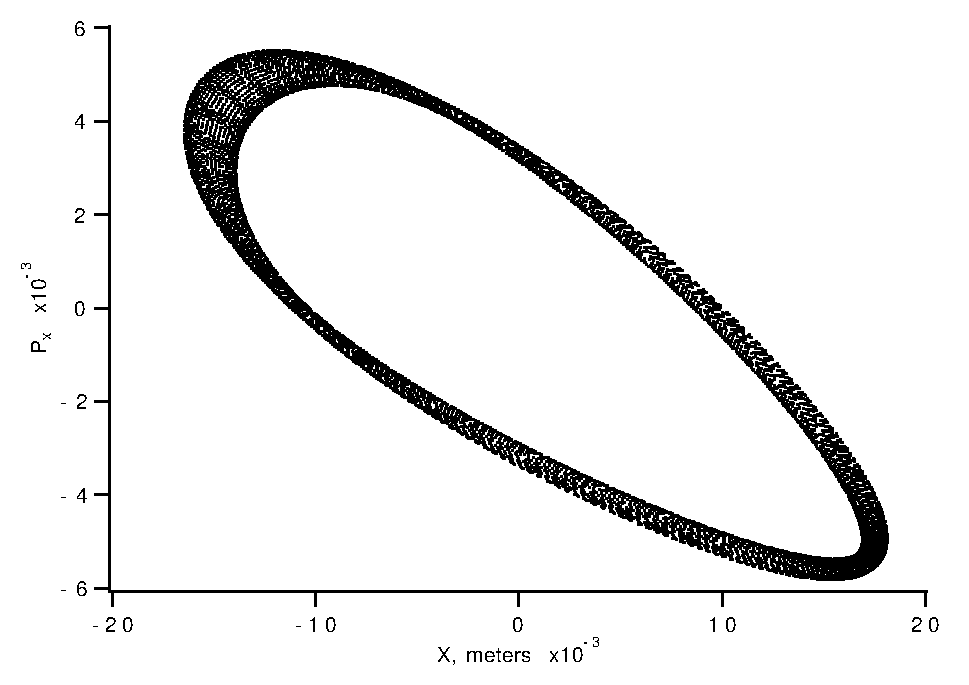
\includegraphics[height=2.69in]{fig2_5_5}
  \caption{Horizontal phase-space projection for
                  trajectory of a single particle in a ring
                              with sextupoles.}
\end{figure}

\begin{figure}[hp]
  \centering
  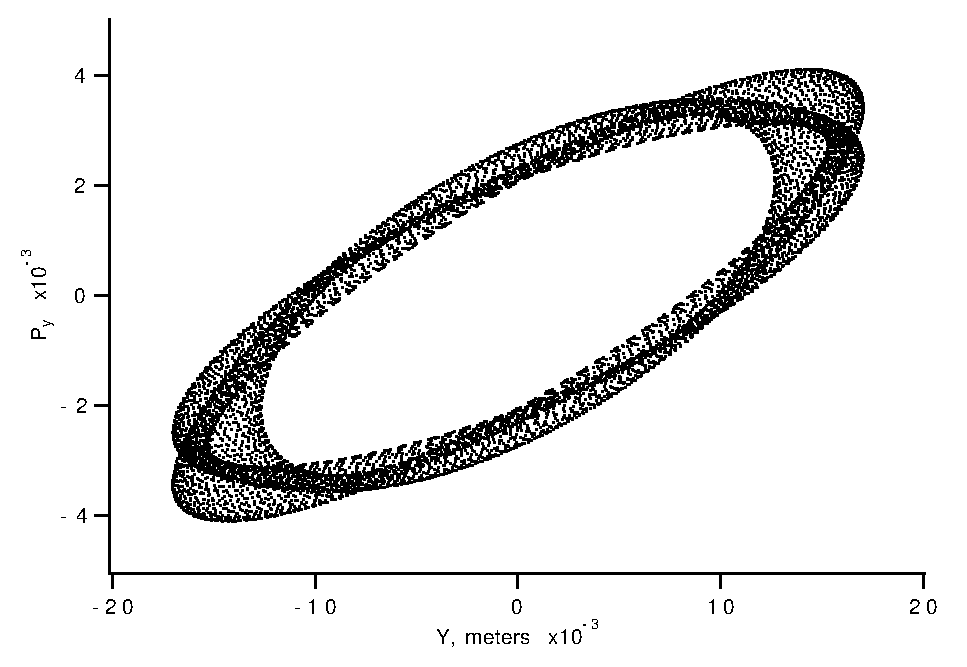
\includegraphics[height=2.69in]{fig2_5_6}
  \caption{Vertical phase-space projection for
                  trajectory of a single particle in a ring
                              with sextupoles.}
\end{figure}

\clearpage
\section{Small Storage Ring with Bunchers}
\label{ringbunchers}
     The example of the small static storage ring treated a time
independent system.  The purpose of this section is to give an example of
the application of \Mary to a time dependent system.  This system will be
a small electron storage ring with radio frequency bunching cavities.  It
is patterned after a design under consideration for construction at
Karlsruhe.  (In actuality, the Los Alamos Proton Storage Ring, upon which
the small static storage ring example of section 2.5 was modeled, also has radio frequency
cavities.  However, their effect was ignored in order to simplify the
earlier discussion.)

     Consider the small electron storage ring shown in figure 2.6.1.\index{storage ring}  It is
designed to circulate approximately 1.4 GeV electrons for the production of
synchrotron radiation.  The ring consists of 4 identical arcs and two radio
frequency cavities.  Each arc is composed of various drifts, a $90^{\circ}$
superconducting bending magnet, 4 quadrupoles, and 2 sextupoles (not
shown). The lattice has 4-fold symmetry when the cavities are turned off,
and 2-fold symmetry when they are identically powered.\index{buncher} \index{cavity} \index{RF cavity}


\begin{figure}[hbp]
  \centering
  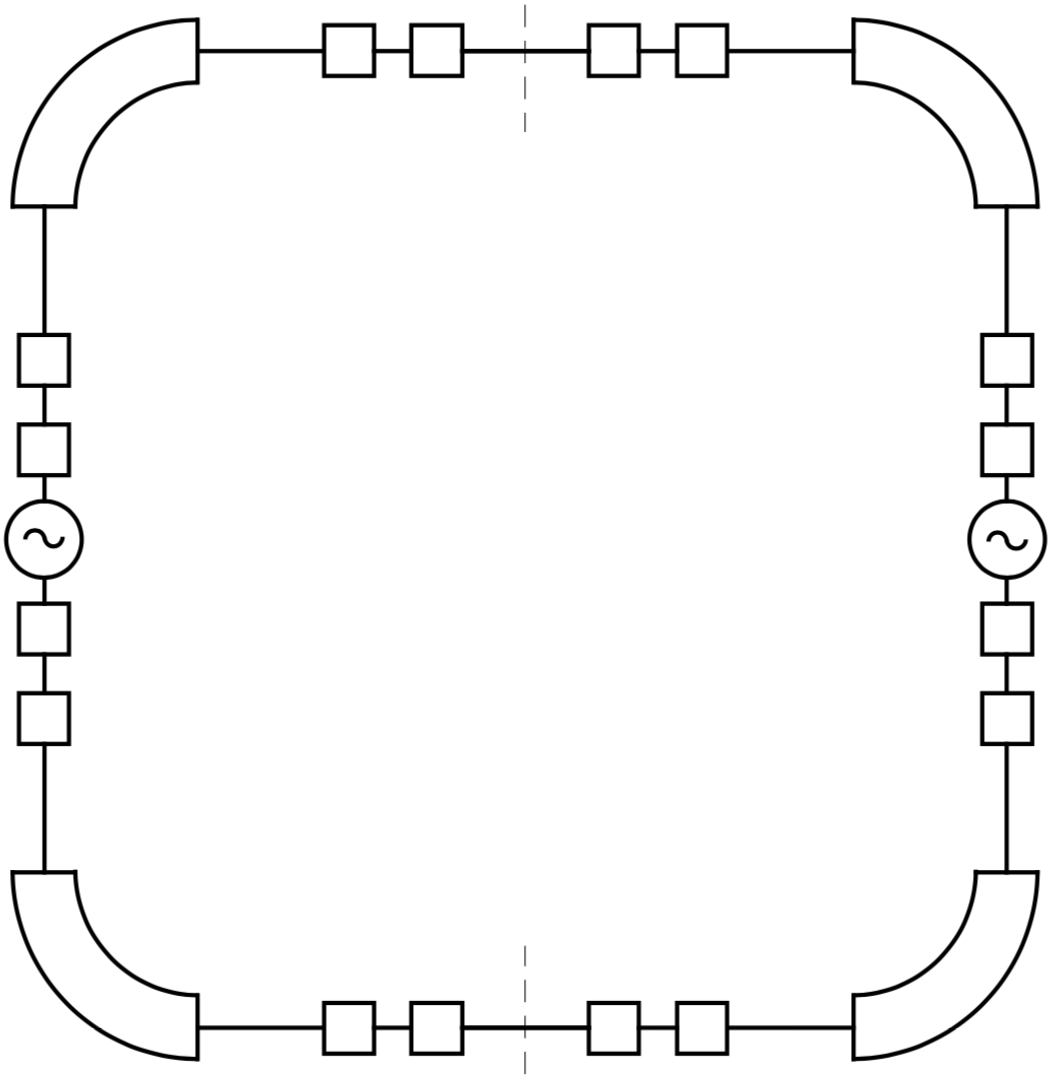
\includegraphics[scale=0.453]{ElectronLayout}
  \caption{Layout of Electron Storage Ring illustrating
                          4 arcs and 2 RF cavities.}
\end{figure}


    The content of an arc is shown in figure 2.6.2.  Note that the arc has
reflection symmetry about the center of the dipole if the effect of the
sextupoles is ignored.

\begin{figure}[htbp]
  \centering
  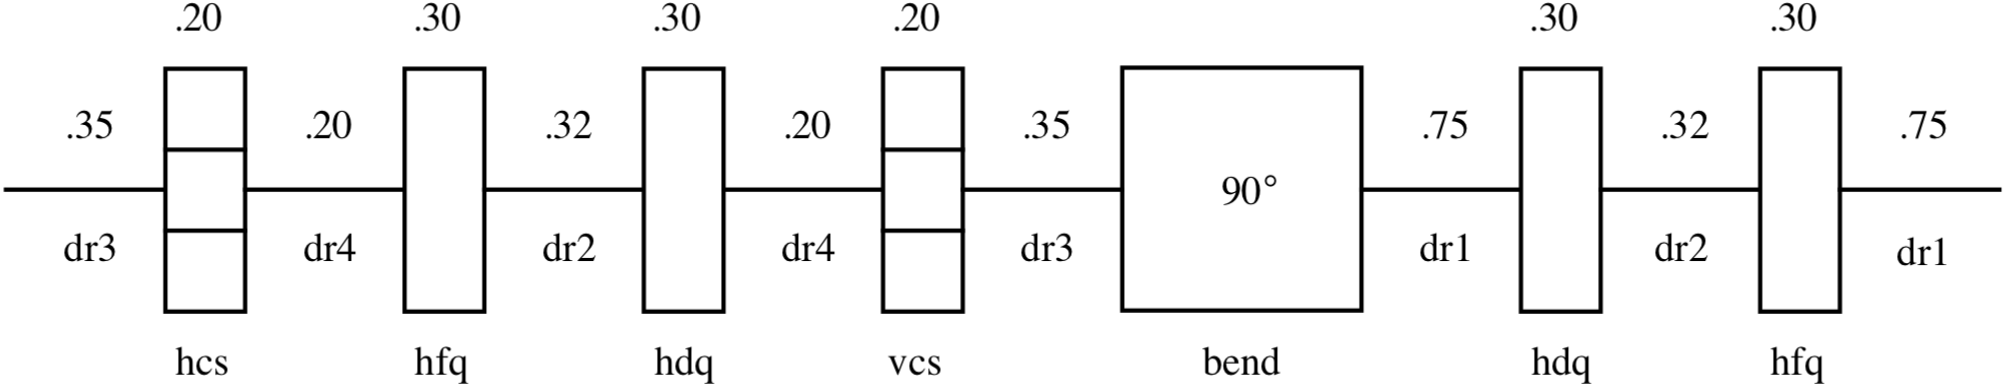
\includegraphics[scale=0.453]{ElectronRing}
  \caption{Details and dimensions of arc for the Electron Storage Ring.  The sextupoles
shown here are not shown in figure 2.6.1.}
\end{figure}

     The results of a \Mary run to study various aspects of this ring are
shown below.  The quadrupoles have been set to achieve static horizontal
and vertical tunes of $2.176\ldots$ and $1.118\ldots$, respectively; and the
sextupoles have been set to achieve near zero first-order chromaticities.
\pagebreak

{
\footnotesize\tt
\begin{verbatim}
 #comment
  Exhibit 2.6.1.
  This is a study of a small ring with buncher.
  This MARYLIE run will first calculate the transverse tunes and
  chromaticities for a static ring without RF cavities.  Next it will
  compute all three tunes when the RF cavities are included.
  Finally, it will track for 12,000 turns.
 #beam
   4.787400000236000
   2807.643747712000
   1.000000000000000
   1.000000000000000
 #menu
  dr1      drft
   0.750000000000000
  dr2      drft
   0.320000000000000
  dr3      drft
   0.350000000000000
  dr4      drft
   0.200000000000000
  bend     nbnd
    90.0000000000000      0.000000000000000E+00  0.500000000000000E+00
    4.00000000000000       1.00000000000000       1.00000000000000
  hfq      quad
   0.300000000000000       11.6094450000000       1.00000000000000
    1.00000000000000
  hdq      quad
   0.300000000000000      -11.0110200000000       1.00000000000000
    1.00000000000000
  hcs      sext
   0.200000000000000       8.91000000000000
  vcs      sext
   0.200000000000000      -31.2000000000000
  cvty     srfc
   -350000.000000000       502000000.000000
  chrom    tasm
    2.00000000000000      1.000000000000000E-03   1.00000000000000
   0.000000000000000E+00   3.00000000000000      0.000000000000000E+00
  tunes    tadm
    1.00000000000000      0.000000000000000E+00   3.00000000000000
   0.000000000000000E+00
  raysin   rt
    13.0000000000000       14.0000000000000      0.000000000000000E+00
   0.000000000000000E+00  0.000000000000000E+00  0.000000000000000E+00
  track    rt
   0.000000000000000E+00   14.0000000000000       5.00000000000000
    12000.0000000000       3.00000000000000      0.000000000000000E+00
  fin      end
  mapout   ptm
    3.00000000000000       3.00000000000000      0.000000000000000E+00
   0.000000000000000E+00   1.00000000000000
  fileout  pmif
    1.00000000000000       12.0000000000000       3.00000000000000
  iden     iden
 #lines
  arc
      1*dr3         1*hcs         1*dr4         1*hfq         1*dr2      &
      1*hdq         1*dr4         1*vcs         1*dr3         1*bend     &
      1*dr1         1*hdq         1*dr2         1*hfq         1*dr1
  half
      1*arc         1*cvty        1*arc
  statring
      4*arc
  dynring
      2*half
 #lumps
 #loops
 #labor
     1*fileout
     1*statring
     1*chrom
     1*mapout
     1*iden
     1*dynring
     1*tunes
     1*mapout
     1*raysin
     1*track
     1*fin

 twiss analysis of static map

 tunes and chromaticities for delta defined in terms of momentum deviation:
 horizontal tune =  0.1767754018607071
 first order horizontal chromaticity =  8.4331690833771913E-04
 second order horizontal chromaticity =   61.84375239529651
 horizontal tune when delta =  9.9999999999999999E-04
  0.1768380889300107

 vertical tune =  0.1187408593290881
 first order vertical chromaticity = -5.0971918876900108E-04
 second order vertical chromaticity =   50.75190581253528
 vertical tune when delta =  9.9999999999999999E-04
  0.1187911015157119

 tune separation when delta=  9.9999999999999999E-04
  5.8046987414298845E-02

 normalized anharmonicities
  hhn=   26.37172974127064
  vvn=   68.90926349103454
  hvn=  -161.4909890590244

 matrix for map is :

 4.44023E-01 7.63417E+00  0.00000E+00 0.00000E+00  0.00000E+00 -1.01718E+00
-1.05164E-01 4.44023E-01  0.00000E+00 0.00000E+00  0.00000E+00 -1.92402E-01
 0.00000E+00 0.00000E+00  7.34361E-01 1.41205E+00  0.00000E+00  0.00000E+00
 0.00000E+00 0.00000E+00 -3.26273E-01 7.34361E-01  0.00000E+00  0.00000E+00
 1.92402E-01 1.01718E+00  0.00000E+00 0.00000E+00  1.00000E+00 -1.94986E+00
 0.00000E+00 0.00000E+00  0.00000E+00 0.00000E+00  0.00000E+00  1.00000E+00

 nonzero elements in generating polynomial are :

  f( 28)=f( 30 00 00 )= 0.45215379538286D-01
  f( 29)=f( 21 00 00 )=-0.22046694853331D+00
  f( 33)=f( 20 00 01 )= 0.21307843039387D-01
  f( 34)=f( 12 00 00 )=-0.34001019319329D+01
  f( 38)=f( 11 00 01 )=-0.80852510867486D+01
  f( 39)=f( 10 20 00 )=-0.23700155752496D+01
  f( 40)=f( 10 11 00 )=-0.72221004647340D+01
  f( 43)=f( 10 02 00 )= 0.99716164303407D+01
  f( 48)=f( 10 00 02 )=-0.24163272701699D+00
  f( 49)=f( 03 00 00 )= 0.24871284484431D+02
  f( 53)=f( 02 00 01 )= 0.10293038577256D+02
  f( 54)=f( 01 20 00 )= 0.50118468271474D+01
  f( 55)=f( 01 11 00 )=-0.44809549519846D+01
  f( 58)=f( 01 02 00 )= 0.10485631631995D+02
  f( 63)=f( 01 00 02 )=-0.10110704197038D+02
  f( 67)=f( 00 20 01 )=-0.43240254040841D+01
  f( 70)=f( 00 11 01 )=-0.14604513970980D+02
  f( 76)=f( 00 02 01 )= 0.18184820623932D+02
  f( 83)=f( 00 00 03 )=-0.30157132940637D+01
  f( 84)=f( 40 00 00 )=-0.81736280922983D+00
  f( 85)=f( 31 00 00 )= 0.11682773681669D+02
  f( 89)=f( 30 00 01 )=-0.57373843211935D+01
  f( 90)=f( 22 00 00 )=-0.10667462524008D+03
  f( 94)=f( 21 00 01 )= 0.57774080071438D+02
  f( 95)=f( 20 20 00 )= 0.10610937449426D+02
  f( 96)=f( 20 11 00 )=-0.25346373720784D+02
  f( 99)=f( 20 02 00 )=-0.17887202924927D+01
  f(104)=f( 20 00 02 )=-0.33795119642547D+02
  f(105)=f( 13 00 00 )= 0.55094300709058D+03
  f(109)=f( 12 00 01 )=-0.34940813399429D+03
  f(110)=f( 11 20 00 )= 0.47360502589164D+02
  f(111)=f( 11 11 00 )=-0.35352607194411D+02
  f(114)=f( 11 02 00 )= 0.16557547039968D+03
  f(119)=f( 11 00 02 )= 0.25564377797871D+03
  f(123)=f( 10 20 01 )= 0.54619011834984D+02
  f(126)=f( 10 11 01 )=-0.14758283906768D+03
  f(132)=f( 10 02 01 )=-0.72171909711283D+02
  f(139)=f( 10 00 03 )=-0.82876422714614D+02
  f(140)=f( 04 00 00 )=-0.12623673101388D+04
  f(144)=f( 03 00 01 )= 0.11300019453141D+04
  f(145)=f( 02 20 00 )=-0.11207086004803D+03
  f(146)=f( 02 11 00 )= 0.28089975149293D+03
  f(149)=f( 02 02 00 )=-0.85697906810901D+03
  f(154)=f( 02 00 02 )=-0.74989176416074D+03
  f(158)=f( 01 20 01 )= 0.95032003682075D+02
  f(161)=f( 01 11 01 )= 0.46315498241881D+03
  f(167)=f( 01 02 01 )= 0.17210946628600D+03
  f(174)=f( 01 00 03 )= 0.34618343480949D+03
  f(175)=f( 00 40 00 )=-0.39584960702938D+00
  f(176)=f( 00 31 00 )= 0.34012760236674D+02
  f(179)=f( 00 22 00 )=-0.29803015500570D+02
  f(184)=f( 00 20 02 )= 0.22800959614659D+02
  f(185)=f( 00 13 00 )=-0.13414827063085D+03
  f(190)=f( 00 11 02 )=-0.16360310517214D+03
  f(195)=f( 00 04 00 )= 0.41037425482445D+02
  f(200)=f( 00 02 02 )=-0.29158811088700D+03
  f(209)=f( 00 00 04 )=-0.82952558576731D+02

 twiss analysis of dynamic map

 horizontal tune =  0.1766133182729722
 vertical tune =  0.1187408593290881
 temporal tune = -1.7314966426091506E-02

 normalized anharmonicities
  hhn=   26.32234081842545
  vvn=   68.66906498937427
  ttn=   2.564081220741627
  hvn=  -161.0403476609988
  htn=  0.8264933075857925
  vtn=  0.5946233516118033

 matrix for map is :

 4.45947E-01 7.57790E+00  0.00000E+00 0.00000E+00 -1.70376E-02 -9.93256E-01
-1.05212E-01 4.45947E-01  0.00000E+00 0.00000E+00  5.58342E-04 -1.92985E-01
 0.00000E+00 0.00000E+00  7.34361E-01 1.41205E+00  0.00000E+00  0.00000E+00
 0.00000E+00 0.00000E+00 -3.26273E-01 7.34361E-01  0.00000E+00  0.00000E+00
 1.92985E-01 9.93256E-01  0.00000E+00 0.00000E+00  9.93076E-01 -1.94279E+00
-5.58342E-04 1.70376E-02  0.00000E+00 0.00000E+00  5.12524E-03  9.93076E-01
 nonzero elements in generating polynomial are :

  f( 28)=f( 30 00 00 )= 0.45272402371279D-01
  f( 29)=f( 21 00 00 )=-0.21619291913033D+00
  f( 32)=f( 20 00 10 )= 0.52159116379009D-03
  f( 33)=f( 20 00 01 )= 0.22809711783722D-01
  f( 34)=f( 12 00 00 )=-0.33266111187308D+01
  f( 37)=f( 11 00 10 )= 0.27446242180918D-01
  f( 38)=f( 11 00 01 )=-0.80348939219789D+01
  f( 39)=f( 10 20 00 )=-0.23721440107942D+01
  f( 40)=f( 10 11 00 )=-0.72230756994141D+01
  f( 43)=f( 10 02 00 )= 0.99743831183019D+01
  f( 46)=f( 10 00 20 )=-0.14198633319081D-04
  f( 47)=f( 10 00 11 )= 0.69285355799949D-02
  f( 48)=f( 10 00 02 )=-0.22958036119541D+00
  f( 49)=f( 03 00 00 )= 0.24283780818181D+02
  f( 52)=f( 02 00 10 )=-0.17675339230659D+00
  f( 53)=f( 02 00 01 )= 0.99501518205640D+01
  f( 54)=f( 01 20 00 )= 0.49357178993046D+01
  f( 55)=f( 01 11 00 )=-0.45466022612201D+01
  f( 58)=f( 01 02 00 )= 0.10617210625343D+02
  f( 61)=f( 01 00 20 )= 0.37055997589258D-03
  f( 62)=f( 01 00 11 )=-0.27990717530384D-01
  f( 63)=f( 01 00 02 )=-0.10072004315623D+02
  f( 66)=f( 00 20 10 )=-0.22404457233068D-01
  f( 67)=f( 00 20 01 )=-0.43501278829361D+01
  f( 69)=f( 00 11 10 )=-0.18153809343687D-01
  f( 70)=f( 00 11 01 )=-0.14615671070792D+02
  f( 75)=f( 00 02 10 )= 0.37486925842262D-01
  f( 76)=f( 00 02 01 )= 0.18217899125922D+02
  f( 80)=f( 00 00 30 )=-0.11894584377677D-06
  f( 81)=f( 00 00 21 )=-0.27911087363220D-04
  f( 82)=f( 00 00 12 )= 0.24256888920499D-01
  f( 83)=f( 00 00 03 )=-0.29893516527248D+01
  f( 84)=f( 40 00 00 )=-0.81849404478391D+00
  f( 85)=f( 31 00 00 )= 0.11651079604483D+02
  f( 88)=f( 30 00 10 )=-0.13920760824296D-01
  f( 89)=f( 30 00 01 )=-0.57505430076205D+01
  f( 90)=f( 22 00 00 )=-0.10599786106222D+03
  f( 93)=f( 21 00 10 )= 0.24172901812277D+00
  f( 94)=f( 21 00 01 )= 0.58020142165025D+02
  f( 95)=f( 20 20 00 )= 0.10625101726234D+02
  f( 96)=f( 20 11 00 )=-0.25357087882830D+02
  f( 99)=f( 20 02 00 )=-0.17881415870767D+01
  f(102)=f( 20 00 20 )=-0.23139584357480D-02
  f(103)=f( 20 00 11 )=-0.86155728411927D-03
  f(104)=f( 20 00 02 )=-0.33800412976428D+02
  f(105)=f( 13 00 00 )= 0.54463794602174D+03
  f(108)=f( 12 00 10 )=-0.22781682264849D+01
  f(109)=f( 12 00 01 )=-0.35293093264212D+03
  f(110)=f( 11 20 00 )= 0.47692799517677D+02
  f(111)=f( 11 11 00 )=-0.35974719511946D+02
  f(114)=f( 11 02 00 )= 0.16629562793653D+03
  f(117)=f( 11 00 20 )=-0.93974817575462D-01
  f(118)=f( 11 00 11 )=-0.53253606073286D+00
  f(119)=f( 11 00 02 )= 0.25492742947047D+03
  f(122)=f( 10 20 10 )= 0.88421335400037D-01
  f(123)=f( 10 20 01 )= 0.54785968578495D+02
  f(125)=f( 10 11 10 )=-0.12029885863179D+00
  f(126)=f( 10 11 01 )=-0.14784356766062D+03
  f(131)=f( 10 02 10 )= 0.15288776819962D+00
  f(132)=f( 10 02 01 )=-0.72003436494803D+02
  f(136)=f( 10 00 30 )=-0.10249898861021D-01
  f(137)=f( 10 00 21 )=-0.50678910476843D-01
  f(138)=f( 10 00 12 )=-0.11701369149759D+00
  f(139)=f( 10 00 03 )=-0.82981002985973D+02
  f(140)=f( 04 00 00 )=-0.12462350349190D+04
  f(143)=f( 03 00 10 )= 0.19943296100117D+01
  f(144)=f( 03 00 01 )= 0.11328563670199D+04
  f(145)=f( 02 20 00 )=-0.11067647113872D+03
  f(146)=f( 02 11 00 )= 0.27084848589679D+03
  f(149)=f( 02 02 00 )=-0.84834634851423D+03
  f(152)=f( 02 00 20 )=-0.15917450414469D+01
  f(153)=f( 02 00 11 )=-0.39905668810137D+01
  f(154)=f( 02 00 02 )=-0.75350189263427D+03
  f(157)=f( 01 20 10 )= 0.38202021663940D+00
  f(158)=f( 01 20 01 )= 0.96791184584807D+02
  f(160)=f( 01 11 10 )=-0.28565426214560D+01
  f(161)=f( 01 11 01 )= 0.45678847238498D+03
  f(166)=f( 01 02 10 )= 0.24310048159471D+01
  f(167)=f( 01 02 01 )= 0.17905042205389D+03
  f(171)=f( 01 00 30 )=-0.31324939973368D+00
  f(172)=f( 01 00 21 )=-0.12181205220735D+01
  f(173)=f( 01 00 12 )=-0.21760723071158D+01
  f(174)=f( 01 00 03 )= 0.34501431914347D+03
  f(175)=f( 00 40 00 )=-0.39022737321736D+00
  f(176)=f( 00 31 00 )= 0.33968821547973D+02
  f(179)=f( 00 22 00 )=-0.29783342441179D+02
  f(182)=f( 00 20 20 )=-0.38273027582899D-03
  f(183)=f( 00 20 11 )= 0.41191036080077D+00
  f(184)=f( 00 20 02 )= 0.23321286693937D+02
  f(185)=f( 00 13 00 )=-0.13403115928927D+03
  f(188)=f( 00 11 20 )= 0.19164445611293D-02
  f(189)=f( 00 11 11 )=-0.76827567222306D+00
  f(190)=f( 00 11 02 )=-0.16456662147632D+03
  f(195)=f( 00 04 00 )= 0.40941098905118D+02
  f(198)=f( 00 02 20 )=-0.18844971967649D-02
  f(199)=f( 00 02 11 )= 0.10120639947267D+01
  f(200)=f( 00 02 02 )=-0.29069138010614D+03
  f(205)=f( 00 00 40 )=-0.23553455722979D-01
  f(206)=f( 00 00 31 )=-0.12704550327439D+00
  f(207)=f( 00 00 22 )=-0.32046328354160D+00
  f(208)=f( 00 00 13 )=-0.35661776470151D+00
  f(209)=f( 00 00 04 )=-0.83158327801083D+02
\end{verbatim}}

     As indicated in the {\em \#comments} entry, and as can be inferred from
{\em \#labor}, this \Mary run (thanks to the line {\em statring } and the commands
{\em statanal } and {\em chrom}\/) first analyzes the properties of the one-turn transfer
map when the RF cavities are turned off (omitted from the ring).
Inspection of the tunes and chromaticities obtained for this case of a
static ring shows that they do indeed have the desired values.
Subsequently, the one-turn transfer map of the static ring is written out
for future reference.

     Next (thanks to the line {\em dynring } and the command {\em tunes}\/), the
horizontal, vertical, and temporal (synchrotron) tunes are computed for the
time dependent (dynamic) one-turn transfer map.  That the RF cavities are
now included can be seen by observing that the line {\em dynring } is defined in
terms of the line {\em half}, and the line {\em half } includes the element {\em cvty}.
Inspection of the element {\em cvty } in {\em \#menu} shows that it refers to a short
(zero length) RF buncher having a voltage of 350 KeV and a frequency of 502
MHz.  Note that the sign of the cavity voltage is negative, as is
required to achieve stable synchrotron motion, since the ring is
operating above transition.  See section 6.13 and 8.1.

     The effect of the RF cavities can be seen analytically in at least two
ways.  First, observe that the synchrotron tune is nonzero when the
cavities are turned on.  Moreover, comparison of the horizontal tunes for
the static and dynamic rings shows that the introduction of the RF cavities
slightly changes the horizontal tune.  Consequently, there is
synchro-betatron coupling.

     Second, it should be noted that the one-turn transfer maps for the
static and dynamic rings are different.  In particular, the 6,5 entry of
the matrix for the dynamic one-turn transfer map is nonzero.  Also, there
are many more entries in the generating polynomial for the nonlinear part
of the dynamic one-turn transfer map.

     The effect of the RF cavities is also apparent in the phase-space data
generated by the tracking portion of the \Mary run.  The first few lines
of the final condition file (the first line of which is identical to the
initial condition) are listed below.  They are produced by tracking a
single particle for 12,000 turns and writing out the resulting phase-space
coordinates every third turn.  Note that the $P_{\tau}$  phase-space coordinate
(related to the energy) now changes due to synchrotron oscillation.
\vspace{5mm}

    First few lines of final condition file from tracking run
\begin{footnotesize}
\begin{tt}
\begin{tabbing}
-1.699\=89E-07 -4.012\=00E-04 -9.380\=35E-08 -5.491\=85E-05 9.898\=83E-06 0.000\= \kill
\>$X$ \>$P_x$ \>$Y$ \>$P_y$ \>$\tau$ \>$P_{\tau}$
\end{tabbing}
\end{tt}
\vspace{-5mm}
\begin{verbatim}
 0.50000E-02  0.00000E+00  0.50000E-02  0.00000E+00  0.00000E+00  0.10000E-02
-0.75953E-02  0.14178E-03 -0.35432E-02 -0.21199E-02 -0.69645E-02  0.93484E-03
 0.35812E-02 -0.85306E-04 -0.19390E-02  0.26666E-02 -0.12571E-01  0.79454E-03
-0.66481E-02  0.10591E-03  0.52487E-02 -0.70013E-03 -0.17555E-01  0.54973E-03
 0.56676E-02 -0/32624E-03 -0.40548E-02 -0.13211E-02 -0.19619E-01  0.279095E-03
\end{verbatim}
\end{footnotesize}


     Horizontal, vertical, and temporal phase-space projections produced by
plotting the $X,P_x$  and $Y,P_y$  and $\tau,P_{\tau}$  contents of the entire final condition
file are shown in figures 2.6.3, 2.6.4, and 2.6.5.  These figures illustrate two features
that are worthy of attention here.  First, figure 2.6.5 shows that there are
indeed synchrotron oscillations as expected.  Second, all 3 figures indicate
that the 3 phase-space projections, even for a single particle, do not lie on
nice ellipses.  As was the case with the static storage ring, it can be shown
that the ``thickening'' of the horizontal and vertical ellipses is due in part
to nonlinear sextupole effects.  Moreover in this case, the thickening of the
temporal ellipse is due to synchro-betatron coupling, and additional
thickening of the horizontal ellipse is caused by dispersion.

\begin{figure}[hbp]
  \centering
  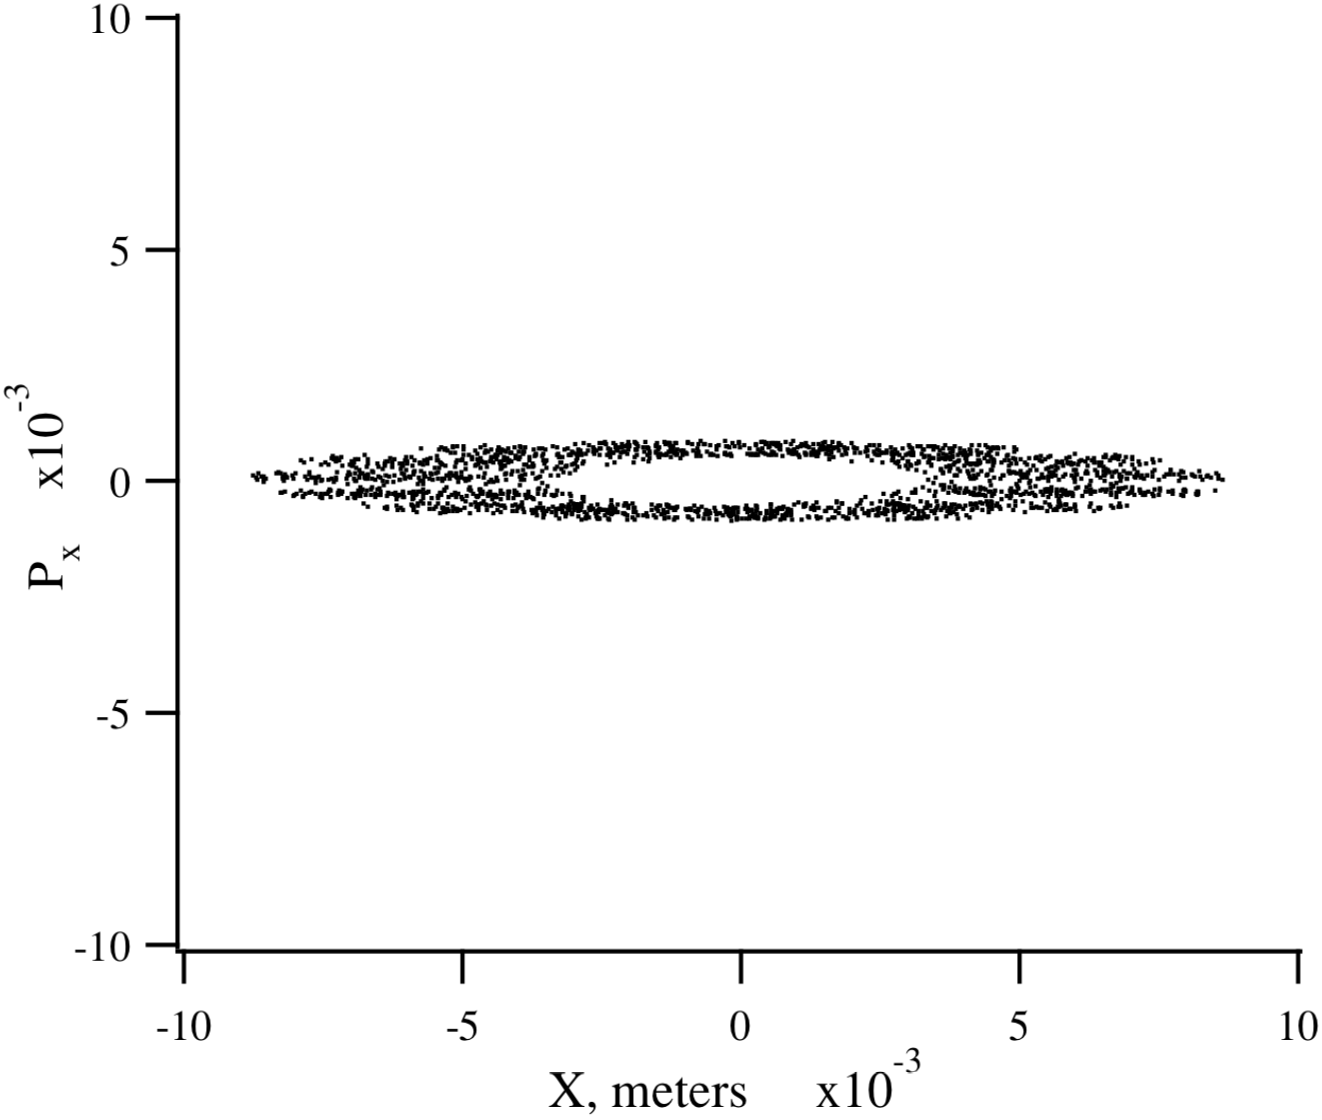
\includegraphics[scale=0.453]{bunch1x}
  \caption{Horizontal phase-space projection for trajectory
       of a single particle in a ring with sextupoles and bunchers.}
\end{figure}

\begin{figure}[hbp]
  \centering
  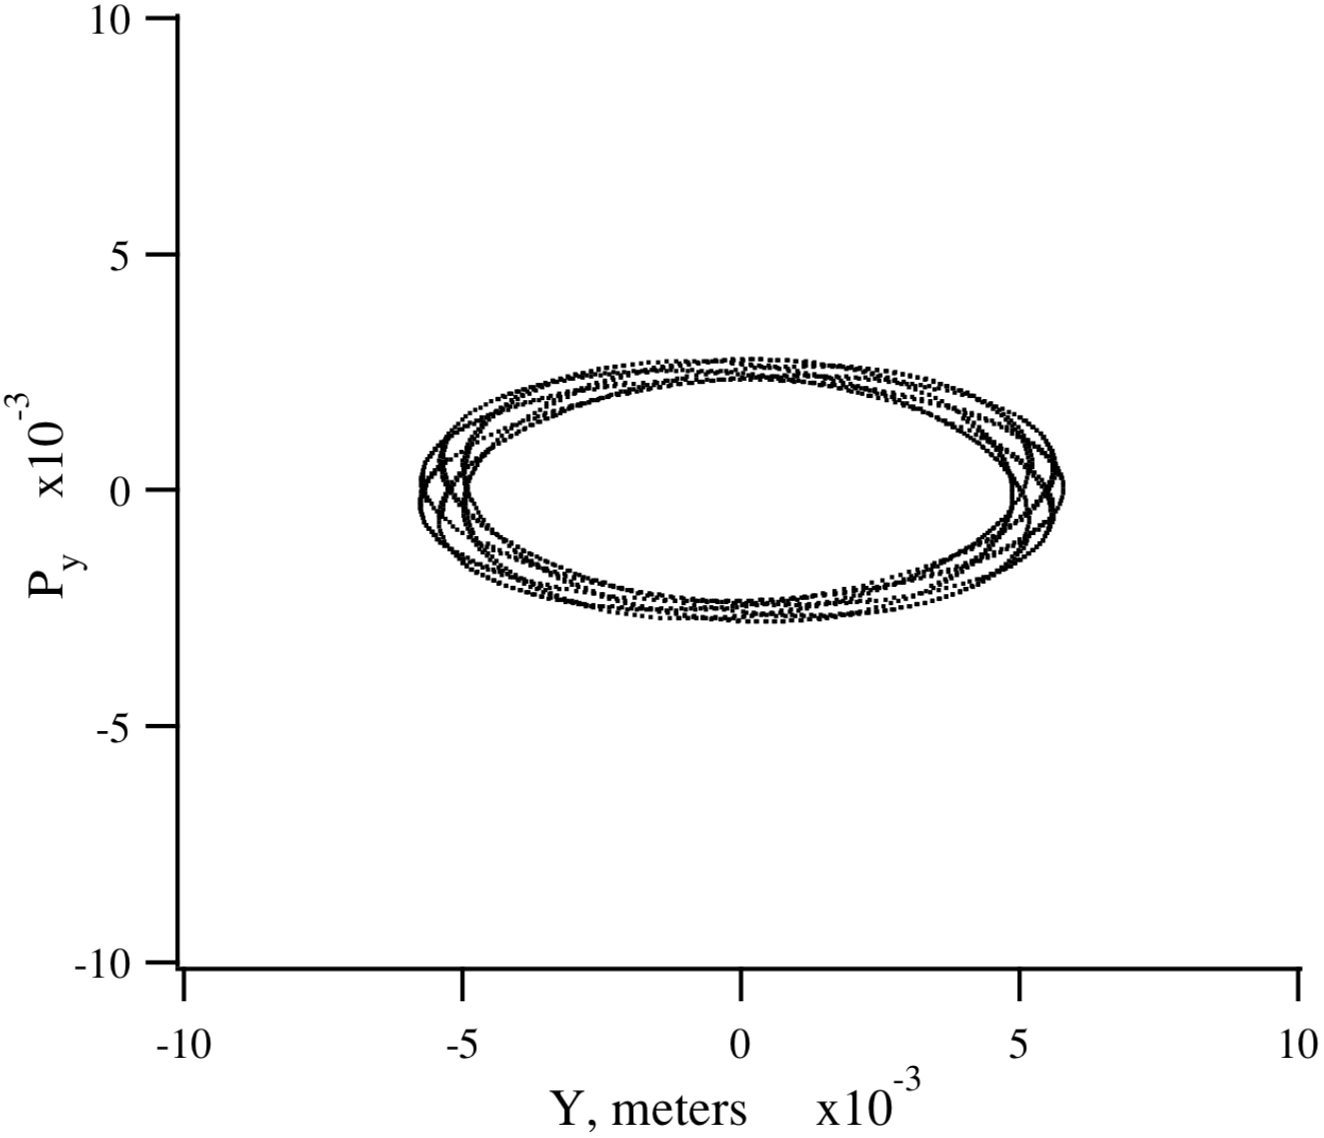
\includegraphics[scale=0.453]{bunch1y}
  \caption{Vertical phase-space projection for trajectory of a
      single particle in a ring with sextupoles and bunchers.}
\end{figure}

\begin{figure}[htbp]
  \centering
  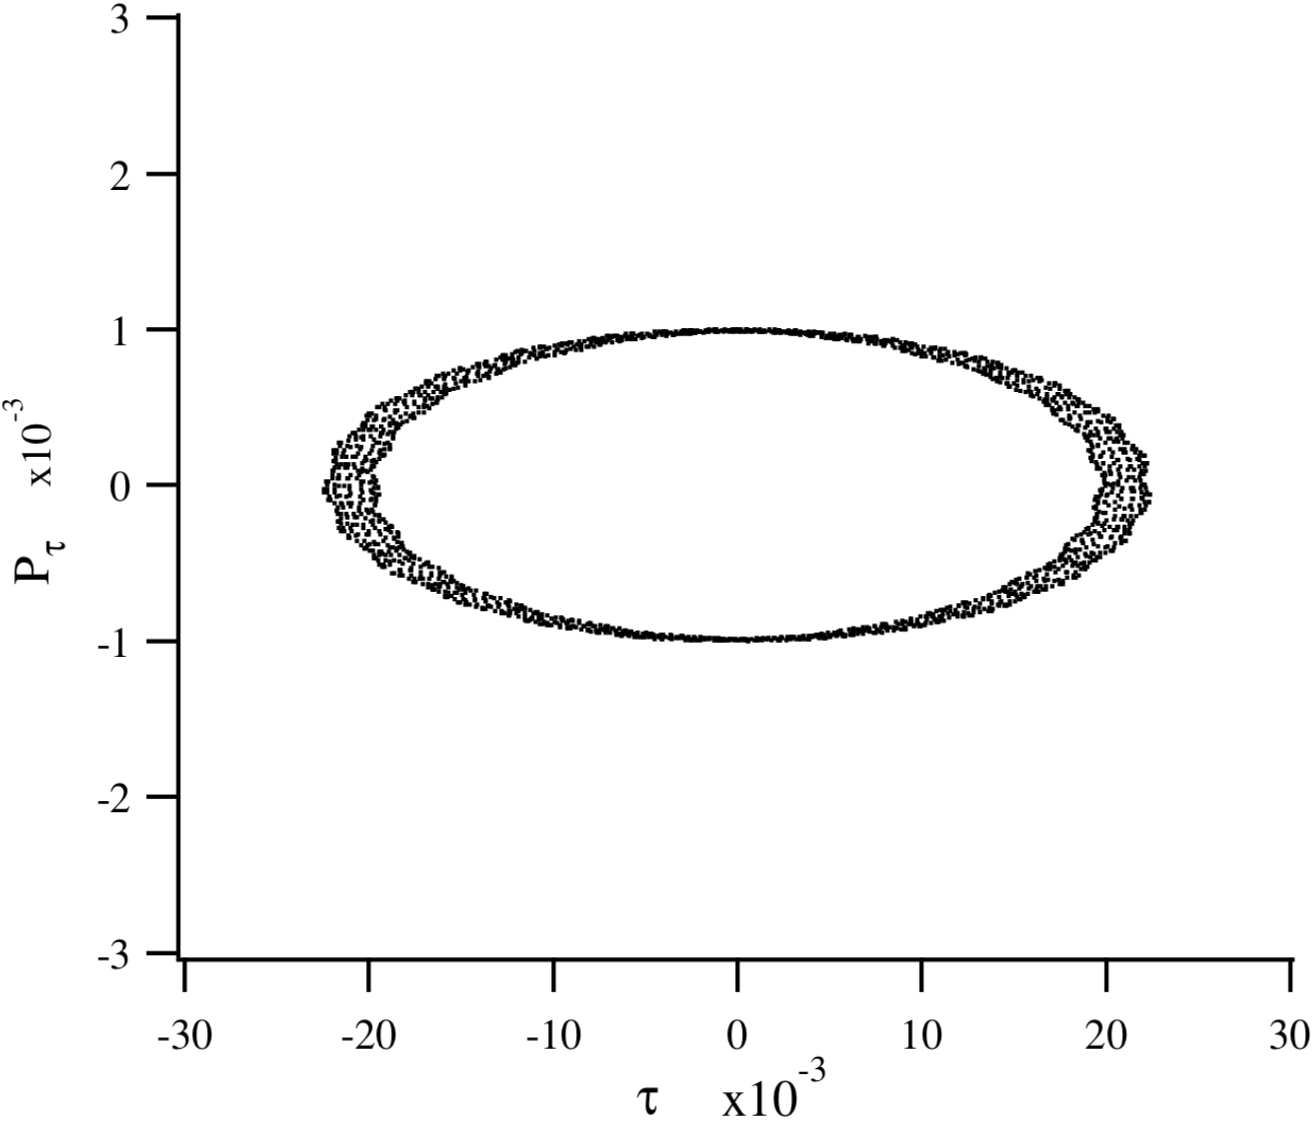
\includegraphics[scale=0.453]{bunch1t}
  \caption{Temporal phase-space projection for trajectory of
       a single particle in a ring with sextupoles and bunchers.}
\end{figure}

     At this point, as with the case of the static storage ring, one may
again wonder about the long-term effect of nonlinearities. One way to
approach this question is to proceed as follows:  In the case of no
nonlinearities, the phase-space trajectory of a stable particle lies on a
3-dimensional torus in 6-dimensional phase space.  (The horizontal,
vertical, and temporal projections of this torus then produce three nice
ellipses.)  One might hope that the addition of small nonlinear effects
simply distorts this torus.\index{torus}  Indeed, the existence of so-called KAM tori
can be proved in some cases.\index{KAM tori}  Moreover, using Lie algebraic techniques, it
is possible to compute the shape such distorted tori would have.  In fact,
it is possible to compute a ``normal form'' transformation map whose inverse
would transform such a distorted torus back into a {\em perfect } torus.
(A perfect torus is the topological product of circles.)  It is
this transformation inverse map that is computed by the commands
{\em dnor}, {\em normap}, and {\em inv}.  See the line {\em cleanup}.
Finally, \Mary could be used to
apply this inverse map to the results of a tracking run, and the
transformed phase-space points thus obtained should lie on a perfect torus.

     The results of following this procedure for the case at hand are illustrated
in the \Mary run shown below.  This run produces tracking data and computes the inverse normalizing map.  The command {\em mapout} prints out this map
to show the reader that the inverse normal form map has nontrivial linear
and nonlinear content.  Finally, this map is applied to the tracking data with the aid of the commands {\em phasein} and {\em xfrmdata}.

{
\footnotesize\tt
\begin{verbatim}
 #comment
  Exhibit 2.6.2.
  This is a study of a small ring with buncher.
  This MARYLIE run will compute the one-turn map and the normalizing map
  (script A) for the dynamic ring.  Then it will track for 12,000 turns.
  Finally, it will apply script A inverse to the tracking (phase space) data.
 #beam
   4.787400000236000
   2807.643747712000
   1.000000000000000
   1.000000000000000
 #menu
  dr1      drft
   0.750000000000000
  dr2      drft
   0.320000000000000
  dr3      drft
   0.350000000000000
  dr4      drft
   0.200000000000000
  bend     nbnd
    90.0000000000000      0.000000000000000E+00  0.500000000000000E+00
    4.00000000000000       1.00000000000000       1.00000000000000
  hfq      quad
   0.300000000000000       11.6094450000000       1.00000000000000
    1.00000000000000
  hdq      quad
   0.300000000000000      -11.0110200000000       1.00000000000000
    1.00000000000000
  hcs      sext
   0.200000000000000       8.91000000000000
  vcs      sext
   0.200000000000000      -31.2000000000000
  cvty     srfc
   -350000.000000000       502000000.000000
  inv      inv
  chrom    tasm
    2.00000000000000      1.000000000000000E-03   1.00000000000000
   0.000000000000000E+00   3.00000000000000      0.000000000000000E+00
  tunes    tadm
    1.00000000000000      0.000000000000000E+00   3.00000000000000
   0.000000000000000E+00
  dnor     dnor
   0.000000000000000E+00  0.000000000000000E+00  0.000000000000000E+00
   0.000000000000000E+00  0.000000000000000E+00
  normap   gbuf
    1.00000000000000       1.00000000000000
  raysin   rt
    13.0000000000000       14.0000000000000      0.000000000000000E+00
   0.000000000000000E+00  0.000000000000000E+00  0.000000000000000E+00
  track    rt
   0.000000000000000E+00   14.0000000000000       5.00000000000000
    12000.0000000000       3.00000000000000      0.000000000000000E+00
  phasein  rt
    14.0000000000000       15.0000000000000     -1.000000000000000E+00
   0.000000000000000E+00  0.000000000000000E+00  0.000000000000000E+00
  xfrmdata rt
   0.000000000000000E+00   15.0000000000000       5.00000000000000
    1.00000000000000       1.00000000000000      0.000000000000000E+00
  fin      end
  mapout   ptm
    3.00000000000000       3.00000000000000      0.000000000000000E+00
   0.000000000000000E+00   1.00000000000000
  fileout  pmif
    1.00000000000000       12.0000000000000       3.00000000000000
  iden     iden
 #lines
  arc
      1*dr3         1*hcs         1*dr4         1*hfq         1*dr2      &
      1*hdq         1*dr4         1*vcs         1*dr3         1*bend     &
      1*dr1         1*hdq         1*dr2         1*hfq         1*dr1
  half
      1*arc         1*cvty        1*arc
  statring
      4*arc
  dynring
      2*half
  cleanup
     dnor  iden  normap  inv  mapout  phasein  xfrmdata
 #lumps
 #loops
 #labor
     1*fileout
     1*dynring
     1*raysin
     1*track
     1*cleanup
     1*fin

 matrix for map is :

 3.42760E-01 -3.85186E-34 -3.04104E-20  1.58120E-20 -9.09186E-19  6.21097E-01
 1.06109E-17  2.91212E+00  6.12098E-20 -3.18262E-20 -2.96632E-03  3.74484E-17
 3.85291E-17 -2.27930E-16  6.93319E-01  0.00000E+00  1.14384E-17  2.82857E-16
 4.12874E-17  1.76283E-16 -4.21693E-17  1.44234E+00  6.66292E-17  1.94556E-17
 8.51799E-18  3.93992E-01 -4.48665E-18  2.33285E-18  2.17430E-01  0.00000E+00
-4.67616E-03 -6.90005E-16  4.10774E-17 -2.13583E-17 -1.81334E-17  4.59072E+00

 nonzero elements in generating polynomial are :

  f( 28)=f( 30 00 00 )=-0.10460366964122D+01
  f( 29)=f( 21 00 00 )= 0.69200308272702D+00
  f( 30)=f( 20 10 00 )= 0.19898531389056D-15
  f( 31)=f( 20 01 00 )=-0.97347766627371D-14
  f( 32)=f( 20 00 10 )=-0.83158066949627D-02
  f( 33)=f( 20 00 01 )= 0.60612509412607D+00
  f( 34)=f( 12 00 00 )= 0.16648016481781D+00
  f( 35)=f( 11 10 00 )= 0.27279872506370D-14
  f( 36)=f( 11 01 00 )= 0.42375978544118D-15
  f( 37)=f( 11 00 10 )= 0.23026162999557D-01
  f( 38)=f( 11 00 01 )= 0.58613392995786D+00
  f( 39)=f( 10 20 00 )= 0.20511507145183D+02
  f( 40)=f( 10 11 00 )=-0.29972861950604D+02
  f( 41)=f( 10 10 10 )=-0.86409166793028D-14
  f( 42)=f( 10 10 01 )= 0.27786813771905D-14
  f( 43)=f( 10 02 00 )=-0.24571580215646D+02
  f( 44)=f( 10 01 10 )=-0.14373908883572D-13
  f( 45)=f( 10 01 01 )=-0.10103670383497D-14
  f( 46)=f( 10 00 20 )= 0.94716588280191D-03
  f( 47)=f( 10 00 11 )= 0.12964325061954D-01
  f( 48)=f( 10 00 02 )=-0.59465760190480D-01
  f( 49)=f( 03 00 00 )=-0.24197396160921D-01
  f( 50)=f( 02 10 00 )=-0.21098197225429D-14
  f( 51)=f( 02 01 00 )=-0.34622240280119D-14
  f( 52)=f( 02 00 10 )= 0.20963195822836D-01
  f( 53)=f( 02 00 01 )=-0.20161635759263D+00
  f( 54)=f( 01 20 00 )= 0.16460477389170D+02
  f( 55)=f( 01 11 00 )= 0.28998616728426D+02
  f( 56)=f( 01 10 10 )= 0.10829774863246D-13
  f( 57)=f( 01 10 01 )= 0.21228854055368D-14
  f( 58)=f( 01 02 00 )=-0.19433941567307D+02
  f( 59)=f( 01 01 10 )=-0.10830474022225D-13
  f( 60)=f( 01 01 01 )= 0.22334003872122D-14
  f( 61)=f( 01 00 20 )= 0.14647159365356D-02
  f( 62)=f( 01 00 11 )=-0.10199373053827D-01
  f( 63)=f( 01 00 02 )=-0.17738193455811D-01
  f( 64)=f( 00 30 00 )=-0.22237968545890D-14
  f( 65)=f( 00 21 00 )=-0.10577369403063D-14
  f( 66)=f( 00 20 10 )= 0.74266804499367D-01
  f( 67)=f( 00 20 01 )= 0.36656647331060D+00
  f( 68)=f( 00 12 00 )= 0.20728918613886D-14
  f( 69)=f( 00 11 10 )=-0.76396352091883D-01
  f( 70)=f( 00 11 01 )= 0.13890161158937D+00
  f( 71)=f( 00 10 20 )= 0.81737494981975D-18
  f( 72)=f( 00 10 11 )= 0.18562798797641D-15
  f( 73)=f( 00 10 02 )= 0.21835856493026D-16
  f( 74)=f( 00 03 00 )=-0.63262946709291D-14
  f( 75)=f( 00 02 10 )=-0.12123175636308D+00
  f( 76)=f( 00 02 01 )= 0.18273761587177D+00
  f( 77)=f( 00 01 20 )=-0.19969271071889D-16
  f( 78)=f( 00 01 11 )= 0.10002559395463D-15
  f( 79)=f( 00 01 02 )= 0.30290671594400D-16
  f( 80)=f( 00 00 30 )=-0.17525279110915D+00
  f( 81)=f( 00 00 21 )=-0.90165480465597D-05
  f( 82)=f( 00 00 12 )=-0.26261509257058D+00
  f( 83)=f( 00 00 03 )= 0.27205651724059D-02
  f( 84)=f( 40 00 00 )= 0.64895158004707D+00
  f( 85)=f( 31 00 00 )=-0.63078289525923D+02
  f( 86)=f( 30 10 00 )= 0.11075828167483D-12
  f( 87)=f( 30 01 00 )= 0.38733655058272D-12
  f( 88)=f( 30 00 10 )= 0.19730226060826D-01
  f( 89)=f( 30 00 01 )= 0.11022865304340D+00
  f( 90)=f( 22 00 00 )=-0.57605066262867D+00
  f( 91)=f( 21 10 00 )=-0.33862756313845D-12
  f( 92)=f( 21 01 00 )= 0.30753675862786D-12
  f( 93)=f( 21 00 10 )=-0.25914603597188D+00
  f( 94)=f( 21 00 01 )= 0.31074041102328D+00
  f( 95)=f( 20 20 00 )=-0.22929114528247D+03
  f( 96)=f( 20 11 00 )= 0.13078909602871D+03
  f( 97)=f( 20 10 10 )=-0.30794334939343D-12
  f( 98)=f( 20 10 01 )=-0.14594010721922D-12
  f( 99)=f( 20 02 00 )=-0.27168370001907D+03
  f(100)=f( 20 01 10 )=-0.47781000303471D-12
  f(101)=f( 20 01 01 )= 0.12308842943721D-12
  f(102)=f( 20 00 20 )= 0.72400292463216D-01
  f(103)=f( 20 00 11 )=-0.17985311762636D+02
  f(104)=f( 20 00 02 )= 0.27908608434503D+00
  f(105)=f( 13 00 00 )=-0.36988524143543D+02
  f(106)=f( 12 10 00 )= 0.17835763545761D-12
  f(107)=f( 12 01 00 )= 0.41731695485390D-12
  f(108)=f( 12 00 10 )= 0.19334186177349D+00
  f(109)=f( 12 00 01 )=-0.40065051923326D+00
  f(110)=f( 11 20 00 )= 0.20520120279298D+03
  f(111)=f( 11 11 00 )= 0.31013799054283D+03
  f(112)=f( 11 10 10 )=-0.75021472111021D-13
  f(113)=f( 11 10 01 )= 0.13695012017578D-13
  f(114)=f( 11 02 00 )= 0.21711188678069D+03
  f(115)=f( 11 01 10 )= 0.18984684498544D-12
  f(116)=f( 11 01 01 )= 0.30265389873074D-13
  f(117)=f( 11 00 20 )= 0.75110205029637D+00
  f(118)=f( 11 00 11 )= 0.32024270651727D-01
  f(119)=f( 11 00 02 )=-0.46166662933022D+01
  f(120)=f( 10 30 00 )= 0.36316852919621D-12
  f(121)=f( 10 21 00 )=-0.39273965881445D-13
  f(122)=f( 10 20 10 )=-0.28267347981104D+02
  f(123)=f( 10 20 01 )= 0.21197033992734D+02
  f(124)=f( 10 12 00 )= 0.39437038957407D-12
  f(125)=f( 10 11 10 )= 0.19233218494030D+02
  f(126)=f( 10 11 01 )= 0.18537290025478D+03
  f(127)=f( 10 10 20 )=-0.41117546018783D-14
  f(128)=f( 10 10 11 )= 0.49428353684671D-13
  f(129)=f( 10 10 02 )= 0.16279858176900D-14
  f(130)=f( 10 03 00 )=-0.15485952548739D-12
  f(131)=f( 10 02 10 )= 0.17189421279801D+02
  f(132)=f( 10 02 01 )=-0.33690145720357D+02
  f(133)=f( 10 01 20 )= 0.96954561663828D-14
  f(134)=f( 10 01 11 )=-0.30591978459213D-13
  f(135)=f( 10 01 02 )= 0.12746563234660D-13
  f(136)=f( 10 00 30 )= 0.55260023701988D+01
  f(137)=f( 10 00 21 )=-0.30169192630793D-01
  f(138)=f( 10 00 12 )=-0.35631152567884D+00
  f(139)=f( 10 00 03 )=-0.40336903343816D-01
  f(140)=f( 04 00 00 )=-0.45693469250418D+00
  f(141)=f( 03 10 00 )=-0.44692845707631D-12
  f(142)=f( 03 01 00 )= 0.20478311095529D-12
  f(143)=f( 03 00 10 )=-0.13035493863339D+00
  f(144)=f( 03 00 01 )=-0.56851306886882D+00
  f(145)=f( 02 20 00 )= 0.21162300673632D+03
  f(146)=f( 02 11 00 )= 0.11091257274726D+03
  f(147)=f( 02 10 10 )=-0.24894743851286D-12
  f(148)=f( 02 10 01 )=-0.10421190733649D-12
  f(149)=f( 02 02 00 )= 0.28935183856521D+03
  f(150)=f( 02 01 10 )=-0.26036453147490D-12
  f(151)=f( 02 01 01 )= 0.78091269768035D-13
  f(152)=f( 02 00 20 )=-0.13578593989600D+00
  f(153)=f( 02 00 11 )=-0.18535719712035D+02
  f(154)=f( 02 00 02 )=-0.21570043691224D+00
  f(155)=f( 01 30 00 )=-0.23661322271043D-12
  f(156)=f( 01 21 00 )= 0.36850780905810D-12
  f(157)=f( 01 20 10 )= 0.16104994058979D+01
  f(158)=f( 01 20 01 )=-0.56892181282795D+02
  f(159)=f( 01 12 00 )=-0.70371945371337D-13
  f(160)=f( 01 11 10 )=-0.42482532637124D+02
  f(161)=f( 01 11 01 )= 0.52043569511038D+02
  f(162)=f( 01 10 20 )=-0.12538448629495D-13
  f(163)=f( 01 10 11 )= 0.32841884726300D-13
  f(164)=f( 01 10 02 )=-0.88716089162818D-14
  f(165)=f( 01 03 00 )= 0.57227401111737D-12
  f(166)=f( 01 02 10 )= 0.19596962487988D+02
  f(167)=f( 01 02 01 )= 0.60883631992542D+02
  f(168)=f( 01 01 20 )= 0.43902563215762D-14
  f(169)=f( 01 01 11 )= 0.26597595968999D-13
  f(170)=f( 01 01 02 )= 0.25601889625554D-14
  f(171)=f( 01 00 30 )=-0.25813399199839D-02
  f(172)=f( 01 00 21 )=-0.16594672191018D+01
  f(173)=f( 01 00 12 )=-0.36820662666965D-02
  f(174)=f( 01 00 03 )= 0.12221350313491D-01
  f(175)=f( 00 40 00 )= 0.12727395025196D+02
  f(176)=f( 00 31 00 )= 0.89783562113194D+02
  f(177)=f( 00 30 10 )= 0.16641883626633D-12
  f(178)=f( 00 30 01 )= 0.76428316260937D-13
  f(179)=f( 00 22 00 )=-0.86484837939725D+02
  f(180)=f( 00 21 10 )= 0.13322081000687D-12
  f(181)=f( 00 21 01 )=-0.24050556036498D-13
  f(182)=f( 00 20 20 )= 0.45911287467622D-01
  f(183)=f( 00 20 11 )=-0.17484947380742D+02
  f(184)=f( 00 20 02 )=-0.39878282615400D+00
  f(185)=f( 00 13 00 )=-0.19935210012102D+03
  f(186)=f( 00 12 10 )=-0.86440268094447D-14
  f(187)=f( 00 12 01 )= 0.82130084971219D-13
  f(188)=f( 00 11 20 )= 0.43263259560514D-01
  f(189)=f( 00 11 11 )= 0.29449704923219D+00
  f(190)=f( 00 11 02 )=-0.15708199862304D+01
  f(191)=f( 00 10 30 )=-0.17342752562997D-13
  f(192)=f( 00 10 21 )=-0.32687067290678D-14
  f(193)=f( 00 10 12 )=-0.29825195346950D-13
  f(194)=f( 00 10 03 )=-0.80511602524577D-15
  f(195)=f( 00 04 00 )= 0.16100884288046D+02
  f(196)=f( 00 03 10 )= 0.18642238791199D-12
  f(197)=f( 00 03 01 )=-0.48128094689396D-13
  f(198)=f( 00 02 20 )= 0.14478186615918D-01
  f(199)=f( 00 02 11 )=-0.17410223098787D+02
  f(200)=f( 00 02 02 )= 0.33839335207046D+00
  f(201)=f( 00 01 30 )= 0.45114594483085D-14
  f(202)=f( 00 01 21 )=-0.16264690824082D-13
  f(203)=f( 00 01 12 )= 0.40966025123915D-14
  f(204)=f( 00 01 03 )=-0.16660736068576D-14
  f(205)=f( 00 00 40 )=-0.89667175754049D-03
  f(206)=f( 00 00 31 )= 0.61215249623609D+02
  f(207)=f( 00 00 22 )= 0.33779619515527D-03
  f(208)=f( 00 00 13 )= 0.36555246487907D+02
  f(209)=f( 00 00 04 )= 0.78407302582081D-03
\end{verbatim}}

     Figures 2.6.6, 2.6.7, and 2.6.8 show the $X$,$P_x$  and $Y$,$P_y$  and $\tau$,$P_\tau$  projections of the
transformed phase-space data produced by plotting the final condition file
of this second \Mary run.  Remarkably, all 3 plots are nearly perfect
circles! Correspondingly, the transformed phase-space data lies on a nearly
perfect torus.  Thus, in this case, the thickening of the original ellipses
in figures 2.6.3, 2.6.4, and 2.6.5 is due to apparently harmless nonlinear effects that
can be understood in terms of a Lie algebraically computable map.  This
example illustrates that the ability to remove harmless nonlinear effects
from phase-space data is an important tool for tracking studies, for one
can then examine on a much finer scale whatever chaotic behavior might
remain.

\begin{figure}[hbp]
  \centering
  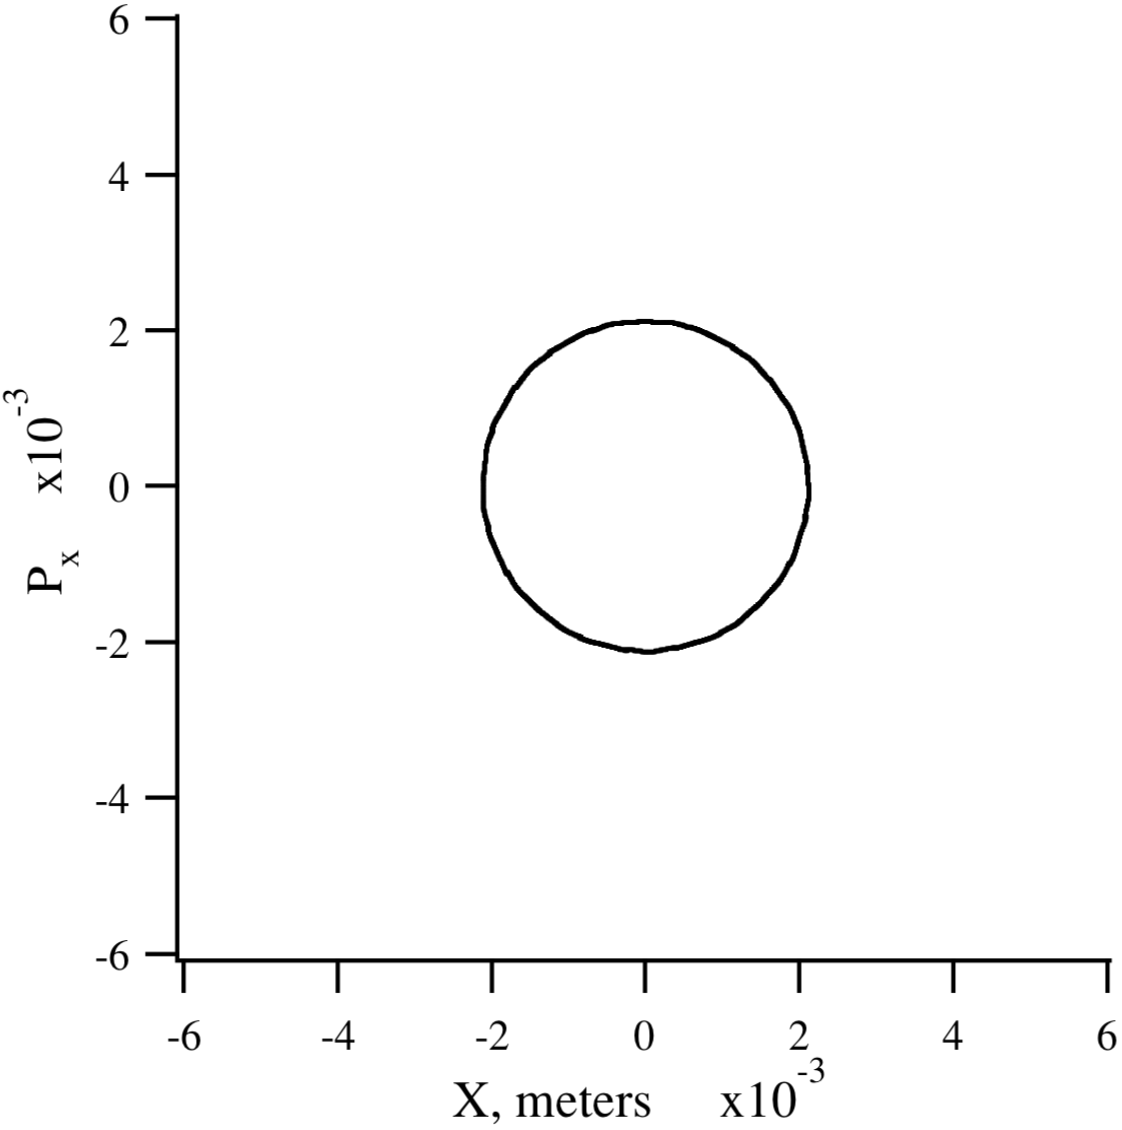
\includegraphics[scale=0.453]{bunch2x}
  \caption{Horizontal projection of transformed phase-space data.}
\end{figure}


\begin{figure}[hbp]
  \centering
  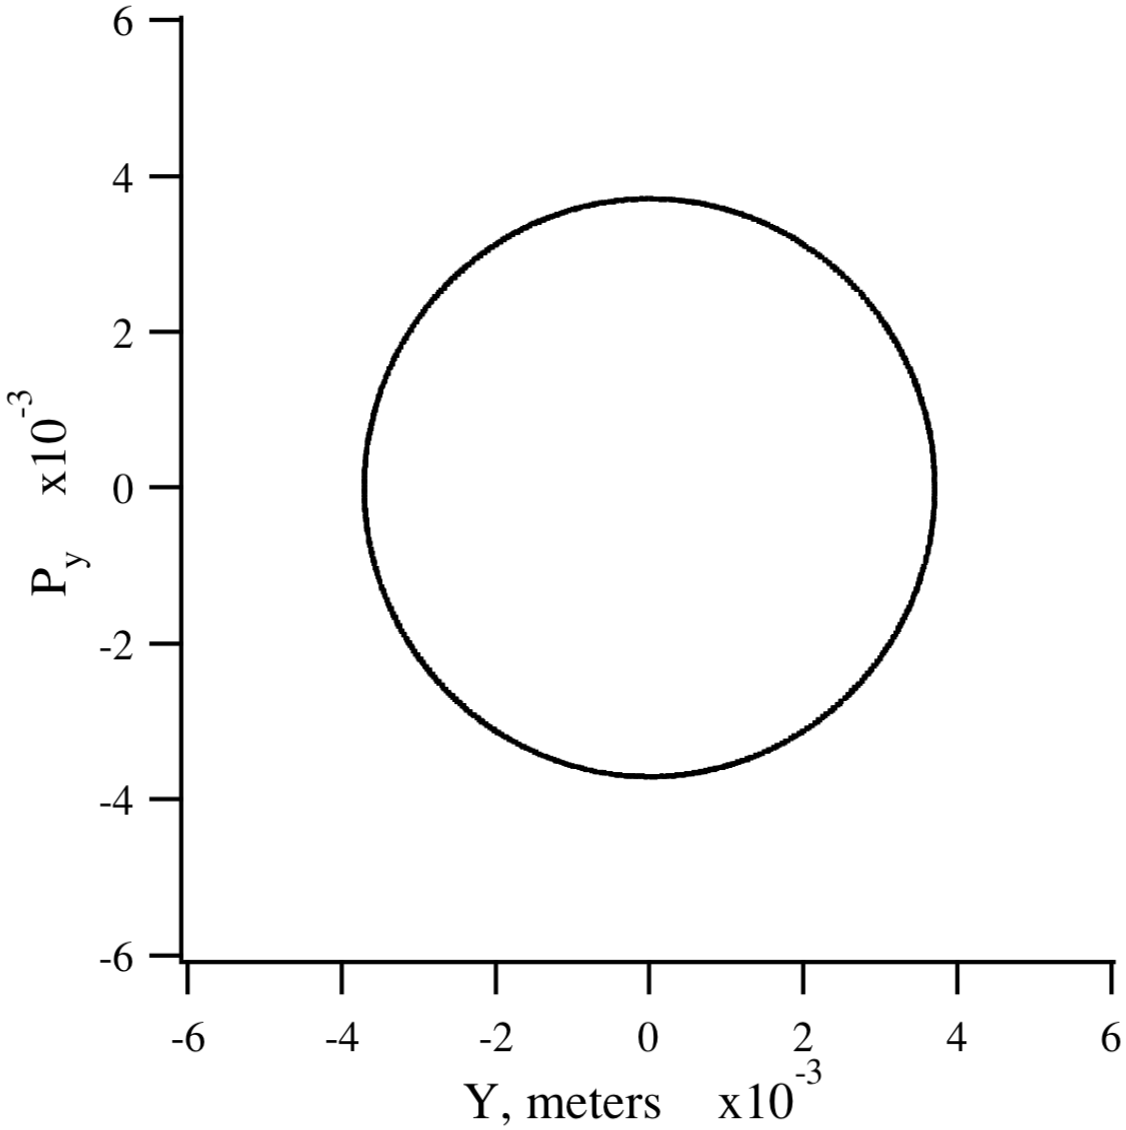
\includegraphics[scale=0.453]{bunch2y}
  \caption{Vertical projection of transformed phase-space data.}
\end{figure}


\begin{figure}[hbp]
  \centering
  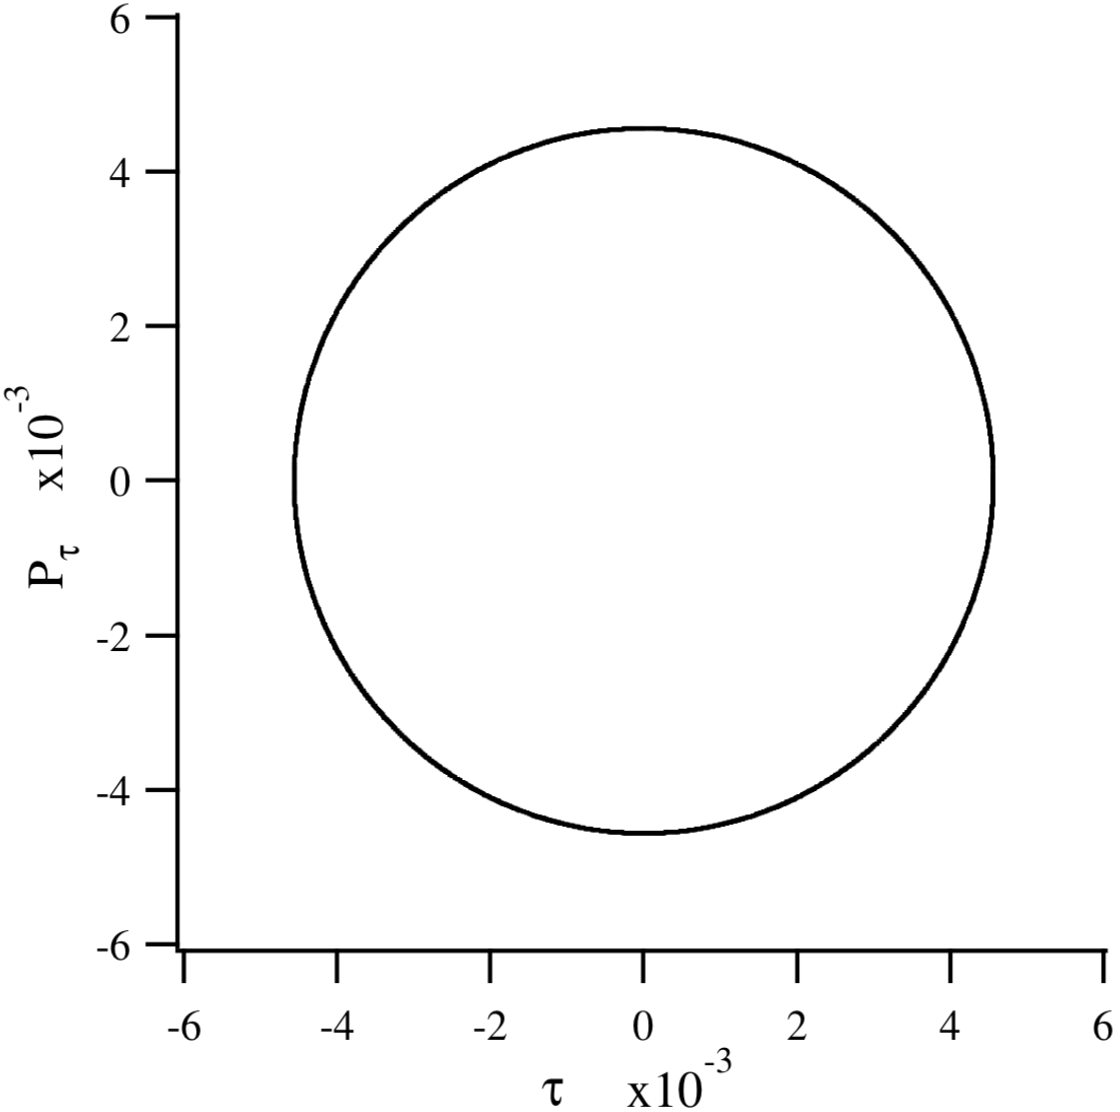
\includegraphics[scale=0.453]{bunch2t}
  \caption{Temporal projection of transformed phase-space data.}
\end{figure}

\clearpage

\section{Large Storage Ring}
\label{largering}
     The previous examples dealt with small systems having relatively few
elements.  The purpose of this section is to give an example of the application
of \Mary to a large system having a large number of elements.  In
particular, an illustration will be given of the use of the {\em \#lump} and {\em \#loop}
features of \Maryend.

     Consider the storage ring shown schematically in figure 2.7.1.\index{storage ring}  It is a
preliminary design of a ring for a Superconducting Super Collider\index{Superconducting Super Collider}, and is
intended to store 20 TeV protons.  As illustrated, the design calls for 6
equally spaced interaction points.  For simplicity, it will be assumed that
all 6 portions of the ring between interaction points are identical.  That
is, the ring will be assumed to have 6 identical superperiods.

\begin{figure}[hbp]
  \centering
  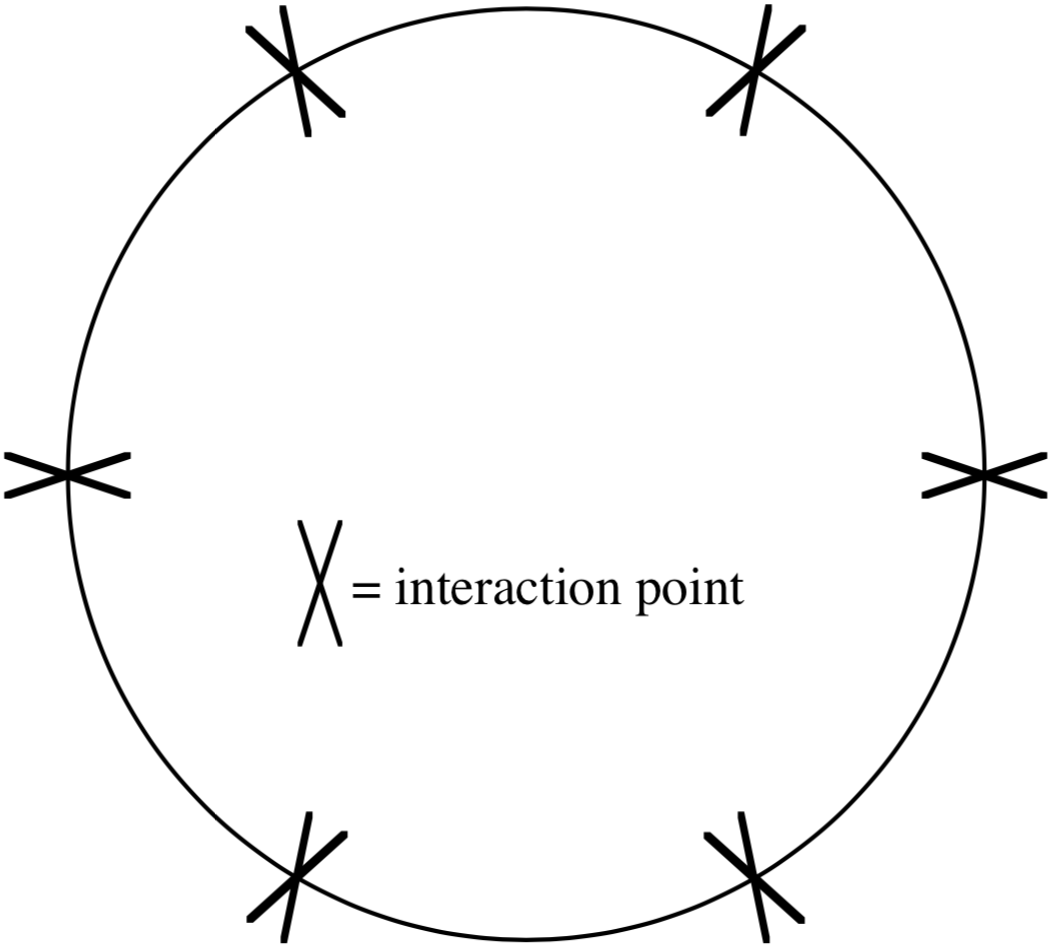
\includegraphics[scale=0.450]{SSCRing}
  \caption{Schematic of Superconducting Super Collider
          storage ring showing 6 equally spaced interaction points
separated by superperiods.}
\end{figure}

     The contents of a superperiod are shown schematically in figure 2.7.2.
It is assumed that both horizontal and vertical beta functions at the
interaction point have the value $\beta^*=1 \mbox{ meter}$.  The section labeled {\em lob1 } is a leading low beta matching section that matches the low beta values at the
interaction point to the larger beta values in the rest of the ring.
Similarly, {\em lob2 } is a trailing low beta section that matches the larger beta
values in the ring to the low values at the interaction point.

\begin{figure}[htbp]
  \centering
  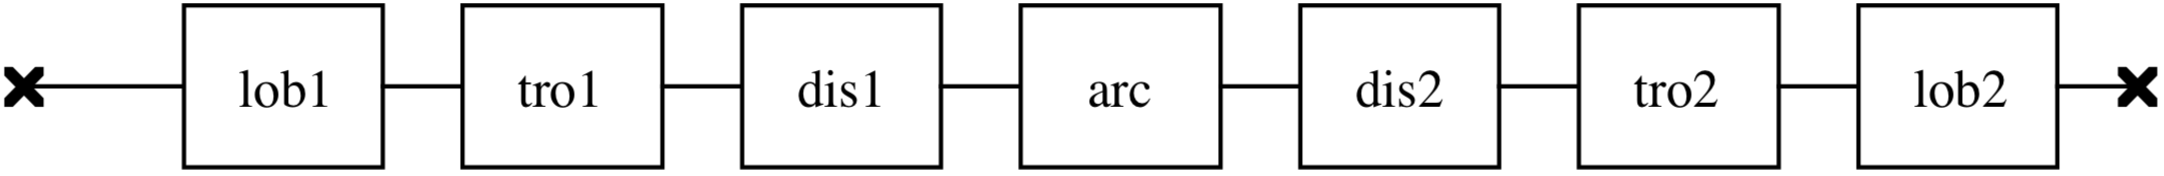
\includegraphics[width=0.98\textwidth]{SSCSuperperiod}
  \caption{Schematic of superperiod for Superconducting
                Super Collider showing its various sections.}
\end{figure}

The sections labeled {\em tro1 } and {\em tro2 } are phase trombones.  They consist
of collections of quadrupoles and drifts, and are used to adjust the tunes
of the ring.\index{phase trombone}

     The sections labeled {\em dis1 } and {\em dis2 } are leading and trailing dispersion
matching sections.  They match the nonzero dispersion values in the section
labeled {\em arc } to zero values at the interaction points, in the low beta
matching sections, and in the phase trombones.

     The arc itself, as shown in figure 2.7.3, consists of two matching
sections labeled {\em arcin } and {\em arcout}, and 60 cells composed of drifts,
dipoles, quadrupoles, and sextupoles.  The arcs provide the major bending
for the ring, and all chromaticity corrections.\index{cell}

\begin{figure}[htbp]
  \centering
  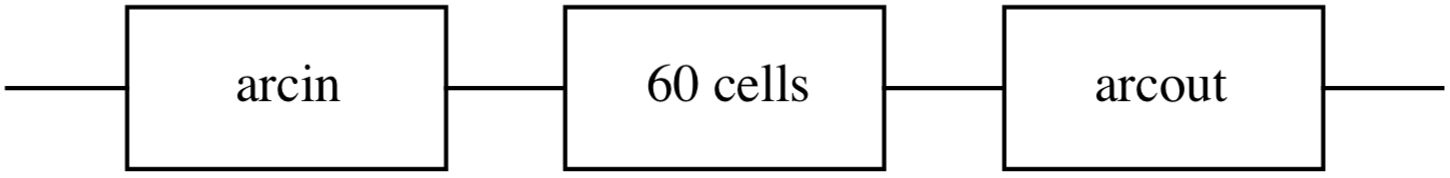
\includegraphics[scale=0.423]{SSCArc}
  \caption{ Schematic of arc for superperiod of
                       Superconducting Super Collider.}
\end{figure}

     Shown below is a \Mary run designed to study various features of
this Superconducting Super Collider design.  Note that {\em \#menu} has now taken
on Chinese proportions.  The contents of a superperiod are listed in the
{\em \#lines} component under the line {\em sixth}, and are as shown in figure
2.7.2.
The contents of the various sections can be seen from the lines {\em lob1}, {\em tro1},
etc., and the various lines and elements to which they refer.  Altogether,
a superperiod consists of 851 elements, and the entire ring consists of
5106 elements.

{
\footnotesize\tt
\begin{verbatim}
 #comment
  Exhibit 2.7.
  This is a study of a large storage ring.
  This MARYLIE run builds up the transfer map for one superperiod (one
  sixth of the ring), prints it out, and computes its tunes and
  chromaticities.
  It also traces rays through one superperiod.
  Then the run tracks for 3000 superperiods (500 turns) using the lump and
  loop features of MARYLIE.  In this case the superperiod is broken up into
  three lumps.
  Each lump contains approximately 40 sextupoles.
 #beam
   66715.94873007700
   21315.60784226800
   1.000000000000000
   1.000000000000000
 #menu
  drc      drft
    5.75000000000000
  drs      drft
    1.87500000000000
  drts     drft
   0.750000000000000
  drtl     drft
    94.7500000000000
  dr56     drft
    18.0000000000000
  dr34     drft
    120.000000000000
  dr1      drft
    1.00000000000000
  dr45     drft
    18.7000000000000
  drex     drft
    20.0000000000000
  drds     drft
    95.0000000000000
  bend     nbnd
   0.444444444444444      0.000000000000000E+00  0.500000000000000E+00
    6.19780700000000       1.00000000000000       1.00000000000000
  qfa      quad
    2.50000000000000       150.844700000000       1.00000000000000
    1.00000000000000
  qda      quad
    2.50000000000000      -150.844700000000       1.00000000000000
    1.00000000000000
  qfb      quad
    5.00000000000000       149.062900000000       1.00000000000000
    1.00000000000000
  qdb      quad
    5.00000000000000      -149.062900000000       1.00000000000000
    1.00000000000000
  qfc      quad
    5.00000000000000       154.497200000000       1.00000000000000
    1.00000000000000
  qdc      quad
    5.00000000000000      -154.497200000000       1.00000000000000
    1.00000000000000
  qfd      quad
    5.00000000000000       153.572400000000       1.00000000000000
    1.00000000000000
  qdd      quad
    5.00000000000000      -153.572400000000       1.00000000000000
    1.00000000000000
  qf1      quad
    6.80000000000000       294.181400000000       1.00000000000000
    1.00000000000000
  qd1      quad
    6.80000000000000      -294.181400000000       1.00000000000000
    1.00000000000000
  qf2      quad
    10.9000000000000       246.370400000000       1.00000000000000
    1.00000000000000
  qd2      quad
    10.9000000000000      -246.370400000000       1.00000000000000
    1.00000000000000
  qf3      quad
    12.1000000000000       221.969400000000       1.00000000000000
    1.00000000000000
  qd3      quad
    12.1000000000000      -221.969400000000       1.00000000000000
    1.00000000000000
  qf4      quad
    5.80000000000000       175.429200000000       1.00000000000000
    1.00000000000000
  qd4      quad
    5.80000000000000      -175.429200000000       1.00000000000000
    1.00000000000000
  qf5      quad
    12.0000000000000       202.941600000000       1.00000000000000
    1.00000000000000
  qd5      quad
    12.0000000000000      -202.941600000000       1.00000000000000
    1.00000000000000
  qf6      quad
    4.00000000000000       48.0381000000000       1.00000000000000
    1.00000000000000
  qd6      quad
    4.00000000000000      -48.0381000000000       1.00000000000000
    1.00000000000000
  qfh      quad
    2.50000000000000       135.701600000000       1.00000000000000
    1.00000000000000
  qdh      quad
    2.50000000000000      -135.710300000000       1.00000000000000
    1.00000000000000
  qf       quad
    5.00000000000000       135.701600000000       1.00000000000000
    1.00000000000000
  qd       quad
    5.00000000000000      -135.710300000000       1.00000000000000
    1.00000000000000
  sf       sext
    2.00000000000000       146.192300000000
  sd       sext
    2.00000000000000      -232.556300000000
  chrom    tasm
    2.00000000000000      1.000000000000000E-03   1.00000000000000
   0.000000000000000E+00   3.00000000000000      0.000000000000000E+00
  fin      end
  circ     circ
   0.000000000000000E+00   14.0000000000000       5.00000000000000
    3000.00000000000       1.00000000000000      0.000000000000000E+00
  raysin   rt
    13.0000000000000       14.0000000000000      -1.00000000000000
   0.000000000000000E+00  0.000000000000000E+00  0.000000000000000E+00
  track    rt
   0.000000000000000E+00   14.0000000000000       5.00000000000000
   0.000000000000000E+00   1.00000000000000      0.000000000000000E+00
  fileout  pmif
    1.00000000000000       12.0000000000000       3.00000000000000
  mapout   ptm
    3.00000000000000       3.00000000000000      0.000000000000000E+00
   0.000000000000000E+00   1.00000000000000
  iden     iden
 #lines
  lob1
      1*drex        1*qf1         1*dr1         1*qf1         1*dr1      &
      1*qd2         1*dr1         1*qd2         1*dr1         1*qf3      &
      1*dr34        1*qf4         1*dr45        1*qd5         1*dr56     &
      1*qf6
  tro1
      1*drts        1*qfa         1*drtl        1*qdb         1*drtl     &
      1*qfc         1*drtl        1*qdd         1*drtl        1*qfc      &
      1*drtl        1*qdb         1*drtl        1*qfa         1*drts
  dis1
      1*qfh         1*drc         1*bend        1*drc         1*qd       &
      1*drc         1*bend        1*drc         1*qf          1*drds     &
      1*qd          1*drds
  nsex
      1*qf          1*drc         1*bend        1*drc         1*qd       &
      1*drc         1*bend        1*drc
  arcin
      3*nsex
  cell
      1*qf          1*drs         1*sf          1*drs         1*bend     &
      1*drs         1*sd          1*drs         1*qd          1*drc      &
      1*bend        1*drc
  arcout
      2*nsex        1*qf          1*drc         1*bend        1*drc      &
      1*qd
  dis2
      1*drds        1*qf          1*drds        1*qd          1*drc      &
      1*bend        1*drc         1*qf          1*drc         1*bend     &
      1*drc         1*qdh
  tro2
      1*drts        1*qda         1*drtl        1*qfb         1*drtl     &
      1*qdc         1*drtl        1*qfd         1*drtl        1*qdc      &
      1*drtl        1*qfb         1*drtl        1*qda         1*drts
  lob2
      1*qd6         1*dr56        1*qf5         1*dr45        1*qd4      &
      1*dr34        1*qd3         1*dr1         1*qf2         1*dr1      &
      1*qf2         1*dr1         1*qd1         1*dr1         1*qd1      &
      1*drex
  arc
      1*arcin      60*cell        1*arcout
  sixth
      1*lob1        1*tro1        1*dis1        1*arc         1*dis2     &
      1*tro2        1*lob2
 #lumps
  lu1
      1*lob1        1*tro1        1*dis1        1*arcin      20*cell
  lu2
     20*cell
  lu3
     20*cell        1*arcout      1*dis2        1*tro2        1*lob2
 #loops
  loop1
      1*lu1         1*lu2         1*lu3
 #labor
     1*fileout
     1*sixth
     1*mapout
     1*chrom
     1*raysin
     1*track
     1*loop1
     1*circ
     1*fin

 matrix for map is :

-2.20484E-01 -9.76044E-01  0.00000E+00  0.00000E+00 0.00000E+00  3.31843E-05
 9.75258E-01 -2.18180E-01  0.00000E+00  0.00000E+00 0.00000E+00  9.38706E-05
 0.00000E+00  0.00000E+00 -2.17810E-01 -9.75919E-01 0.00000E+00  0.00000E+00
 0.00000E+00  0.00000E+00  9.75487E-01 -2.20391E-01 0.00000E+00  0.00000E+00
 5.30602E-05  8.43817E-05  0.00000E+00  0.00000E+00 1.00000E+00 -3.08744E+00
 0.00000E+00  0.00000E+00  0.00000E+00  0.00000E+00 0.00000E+00  1.00000E+00

 nonzero elements in generating polynomial are :

  f( 28)=f( 30 00 00 )=-0.45311841613799D-03
  f( 29)=f( 21 00 00 )=-0.42051084540769D-03
  f( 33)=f( 20 00 01 )= 0.29648412108137D+02
  f( 34)=f( 12 00 00 )= 0.10911021904278D-02
  f( 38)=f( 11 00 01 )=-0.95249092944067D+01
  f( 39)=f( 10 20 00 )= 0.11502630453174D-02
  f( 40)=f( 10 11 00 )=-0.18054566777158D-03
  f( 43)=f( 10 02 00 )=-0.15326259212955D-02
  f( 48)=f( 10 00 02 )=-0.55062715297709D+00
  f( 49)=f( 03 00 00 )= 0.24483150102761D-03
  f( 53)=f( 02 00 01 )=-0.29683518290291D+02
  f( 54)=f( 01 20 00 )= 0.54776622918203D-03
  f( 55)=f( 01 11 00 )=-0.18847354118399D-02
  f( 58)=f( 01 02 00 )=-0.57848883740275D-03
  f( 63)=f( 01 00 02 )= 0.23001005099699D+00
  f( 67)=f( 00 20 01 )=-0.24757716825927D+02
  f( 70)=f( 00 11 01 )=-0.33941869234081D+02
  f( 76)=f( 00 02 01 )= 0.24813595098500D+02
  f( 83)=f( 00 00 03 )= 0.12041613026027D+01
  f( 84)=f( 40 00 00 )= 0.53719143669651D+03
  f( 85)=f( 31 00 00 )=-0.65032625055806D+02
  f( 89)=f( 30 00 01 )= 0.13709185308574D+03
  f( 90)=f( 22 00 00 )= 0.11876136002758D+04
  f( 94)=f( 21 00 01 )=-0.15643146269412D+04
  f( 95)=f( 20 20 00 )= 0.45029248023302D+04
  f( 96)=f( 20 11 00 )=-0.46566047360800D+04
  f( 99)=f( 20 02 00 )= 0.32549479751298D+04
  f(104)=f( 20 00 02 )= 0.12224260475573D+04
  f(105)=f( 13 00 00 )= 0.55183722231071D+02
  f(109)=f( 12 00 01 )= 0.12811016337292D+04
  f(110)=f( 11 20 00 )= 0.39631314514662D+04
  f(111)=f( 11 11 00 )= 0.39099667109689D+04
  f(114)=f( 11 02 00 )=-0.42920577299781D+04
  f(119)=f( 11 00 02 )=-0.80112587128335D+04
  f(123)=f( 10 20 01 )= 0.19710683960939D+04
  f(126)=f( 10 11 01 )=-0.35423279001297D+04
  f(132)=f( 10 02 01 )= 0.43932597295168D+03
  f(139)=f( 10 00 03 )= 0.93187862459852D+02
  f(140)=f( 04 00 00 )= 0.94129796938971D+02
  f(144)=f( 03 00 01 )=-0.12848761161860D+03
  f(145)=f( 02 20 00 )= 0.32433986263860D+04
  f(146)=f( 02 11 00 )= 0.43007468516398D+04
  f(149)=f( 02 02 00 )= 0.44206956850141D+04
  f(154)=f( 02 00 02 )=-0.11847696000829D+02
  f(158)=f( 01 20 01 )=-0.63696419838679D+03
  f(161)=f( 01 11 01 )=-0.27452997974719D+03
  f(167)=f( 01 02 01 )= 0.84212462331467D+03
  f(174)=f( 01 00 03 )=-0.52565377323814D+02
  f(175)=f( 00 40 00 )=-0.72806787999036D+02
  f(176)=f( 00 31 00 )=-0.37282112837702D+03
  f(179)=f( 00 22 00 )= 0.69948623624571D+03
  f(184)=f( 00 20 02 )= 0.18516383109418D+04
  f(185)=f( 00 13 00 )=-0.21045575538010D+02
  f(190)=f( 00 11 02 )=-0.77762707818965D+04
  f(195)=f( 00 04 00 )= 0.32523737181351D+03
  f(200)=f( 00 02 02 )=-0.45676194736033D+03
  f(209)=f( 00 00 04 )= 0.46703244054266D+01

 twiss analysis of static map

 tunes and chromaticities for delta defined in terms of momentum deviation:
 horizontal tune =  0.7148060664739763
 first order horizontal chromaticity =  2.2120285662994830E-06
 second order horizontal chromaticity =  -517.6580207488710
 horizontal tune when delta =  9.9999999999999999E-04
  0.7142884106652559

 vertical tune =  0.7148438795599776
 first order vertical chromaticity =  1.1365906773273283E-06
 second order vertical chromaticity =  -569.8755596054544
 vertical tune when delta =  9.9999999999999999E-04
  0.7142740051369628

 tune separation when delta=  9.9999999999999999E-04
  1.4405528293126579E-05

 normalized anharmonicities
  hhn=  -245.3126910141522
  vvn=  -115.7606385786890
  hvn=  -1227.239884296586
 lump lu1      constructed and stored.( 1)
 lump lu2      constructed and stored.( 2)
 lump lu3      constructed and stored.( 3)
 circulating thru loop1:
      1    2    3
\end{verbatim}}

     As indicated in {\em \#comments}, the \Mary run first builds up the
transfer map for one superperiod, prints it out, and computes its tunes and
chromaticities.  This is accomplished by the entries {\em sixth}, {\em mapout}, and
{\em chrom } in the {\em \#labor} component.  Inspection of the generating polynomial for
the nonlinear portion of the superperiod transfer map shows that it has
noticeable nonlinear content as one might expect from the presence of
numerous sextupoles.  Also, inspection of the result of the chromaticity
calculation shows that the sextupoles have been set to achieve negligible
first-order chromaticities.

     The second function of this \Mary run is to track trajectories
through multipole turns around the ring.  The first appearance in {\em \#labor} of
the command {\em rays } causes the writing of the initial conditions into the
final condition file.  The second appearance of {\em rays}, since it follows the
word {\em sixth}, causes \Mary to apply the superperiod transfer map to the
initial conditions and to write the resulting final conditions in the final
condition file.

     Subsequently, the word {\em loop1 } and the command {\em circ } cause \Mary to
circulate 3000 times through the contents of the loop {\em loop1}, and to write
tracking results into the final condition file after each circulation.
(Observe that the parameters associated with the definition of {\em circ } in
{\em \#menu} have the values 3000 and 1.)

     Reference to the {\em \#lump} component of the \Mary Master Input File
shows that it contains the lumps {\em lu1}, {\em lu2}, and {\em lu3}.  A lump is a collection of elements combined together and treated by a single transfer map.  For
example, as listed in its contents, {\em lu1 } refers to a single transfer map
obtained by combining all the maps for all the elements in {\em lob1}, {\em tro1},
{\em dis1}, {\em arcin}, and {\em 20*cell}.  Observe from the output that as \Mary runs, it announces the construction and storage of lumps by name and assigns them
identification numbers for future reference.

     Now look at the contents of {\em loop1 } as listed under {\em \#loops}.  It contains
the lumps {\em lu1}, {\em lu2}, and {\em lu3}.  When \Mary encounters the name of a loop in \#labor followed by a circulation command such as {\em circ}, it applies the
transfer maps contained in the loop over and over again in succession.
(Look at the \Mary output, and observe that it announces the name of the
loop and the identification numbers of the transfer maps through which
circulation is occurring.)  In this case, the first map {\em lu1 } is applied to
the initial conditions.  Next {\em lu2 } is applied to the resulting phase-space
data.  Then {\em lu3 } is applied to the phase-space data resulting from the
previous application of {\em lu2}.  This completes one circulation around the
loop.  The sequence now repeats.  The transfer map {\em lu1 } acts on the results
obtained from the previous application of {\em lu3}, etc., until the prescribed
number of circulations (3000 in this case) have been completed.

     Examination of the combined contents  of {\em lu1}, {\em lu2}, and {\em lu3} shows that it is identical to the contents of the superperiod {\em sixth}.  As a result,
each circulation in this case amounts to tracking through a superperiod.

     Now comes a subtle but important point.  If \Mary 3.0 were exact to
arbitrary order, the result of applying the transfer map for one
superperiod and the result of performing one circulation would be exactly
the same. However, because \Mary 3.0 only works to third order, higher
order results are lost when a series of transfer maps are combined to
produce a net transfer map.  By contrast, when successive transfer maps are
allowed to act numerically on phase-space data, these so-called {\em cross terms}
are retained. Consequently, the result of using 3 lumps for a superperiod
should be more accurate (should retain more high-order terms) than the
result of using a single map.  Indeed, the accuracy should become better
and better the more and smaller the lumps.  Of course, the cost of
computation increases accordingly because the time consuming part of a
tracking calculation is the numerical evaluation of the action of transfer
maps on phase-space data.

     In any given case, it is necessary to experiment to find the optimum
lump size that minimizes computation time without sacrificing too much
accuracy. Shown below are the first few lines of the final condition file
resulting from the present \Mary run.  The first two lines are two
initial conditions.  The next two lines are the result of applying the one
superperiod transfer map to these two initial conditions.  Lines 5 and 6
are the result of the first circulation through the lumps {\em lu1}, {\em lu2},
and {\em lu3} in {\em loop1}.  The remaining lines are the result of subsequent circulations.
\vspace{5mm}

         First few lines of final condition file from tracking run
\begin{footnotesize}
\begin{tt}
\begin{tabbing}
-1.699\=89E-07 -4.012\=00E-04 -9.380\=35E-08 -5.491\=85E-05 9.898\=83E-06 0.000\= \kill
\>$X$ \>$P_x$ \>$Y$ \>$P_y$ \>$\tau$ \>$P_{\tau}$
\end{tabbing}
\end{tt}
\vspace{-5mm}
\begin{verbatim}
 0.30000E-03  0.00000E+00  0.30000E-03  0.00000E+00  0.00000E+00 0.00000E+00
 0.10000E-02  0.00000E+00  0.10000E-02  0.00000E+00  0.00000E+00 0.00000E+00
-0.66366E-04  0.29239E-03 -0.65638E-04  0.29269E-03 -0.43071E-06 0.00000E+00
-0.22862E-03  0.96816E-03 -0.22878E-03  0.97688E-03 -0.52978E-05 0.00000E+00
-0.66366E-04  0.29239E-03 -0.65636E-04  0.29269E-03 -0.43599E-06 0.00000E+00
-0.22867E-03  0.96853E-03 -0.22844E-03  0.97723E-03 -0.59345E-05 0.00000E+00
-0.27052E-03 -0.12874E-03 -0.27133E-03 -0.12879E-03  0.83488E-06 0.00000E+00
-0.88631E-03 -0.44215E-03 -0.90325E-03 -0.44732E-03  0.95155E-05 0.00000E+00
\end{verbatim}
\end{footnotesize}

     Lines 3 and 5, which are the respective results of applying to the
initial condition in line 1 the one superperiod transfer map and one
circulation, are nearly identical.  Lines 4 and 6, which result from
applying the one superperiod transfer map and one circulation to the
initial condition in line 2, differ in the fourth place.  A difference in
accuracy is to be expected for these two initial conditions because the
initial condition in line 2 has larger betatron amplitudes, and
consequently higher order nonlinear effects should then be more important.

     Evidently superperiod by superperiod tracking is sufficiently accurate
for the smaller betatron amplitude case.  Further investigation shows that
breaking up a superperiod into 3 lumps gives sufficient accuracy in the
larger betatron amplitude case.  In actual operation of a Superconducting
Super Collider, the betatron amplitudes would be expected to be an order of
magnitude smaller than even that of the first initial condition.  Thus
\Mary 3.0 superperiod by superperiod tracking of the error-free design
lattice gives excellent accuracy for orbits of physical interest.

     Figures 2.7.4 and 2.7.5 show phase-space plots resulting from the tracking
portion of the \Mary run.  The orbits appear to have long-term stability.
Indeed, much longer tracking runs give similar results.  It should also be
observed that there is considerable braiding and thickening of the
phase-space projections.  Again, as with the examples of the small proton
and small electron rings, this is a nonlinear and presumably harmless
effect due to sextupoles.

\begin{figure}[hbp]
  \centering
  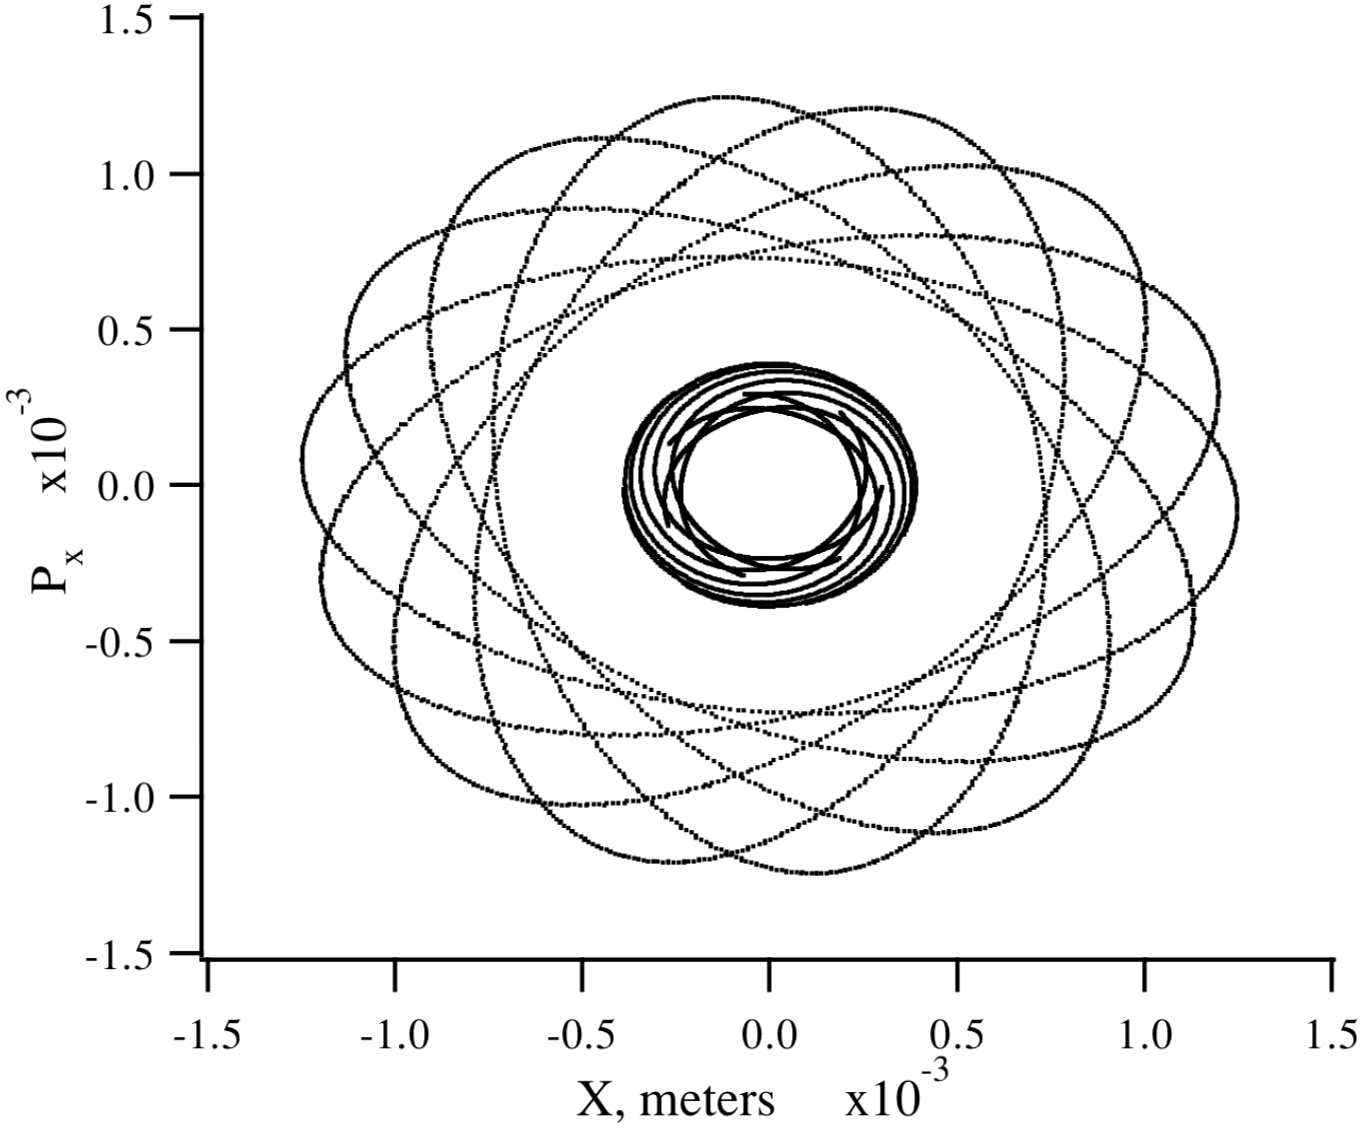
\includegraphics[scale=0.443]{sscx}
  \caption{Horizontal phase-space projection for trajectories
      of two particles in a Superconducting Super Collider.}
\end{figure}


\begin{figure}[hbp]
  \centering
  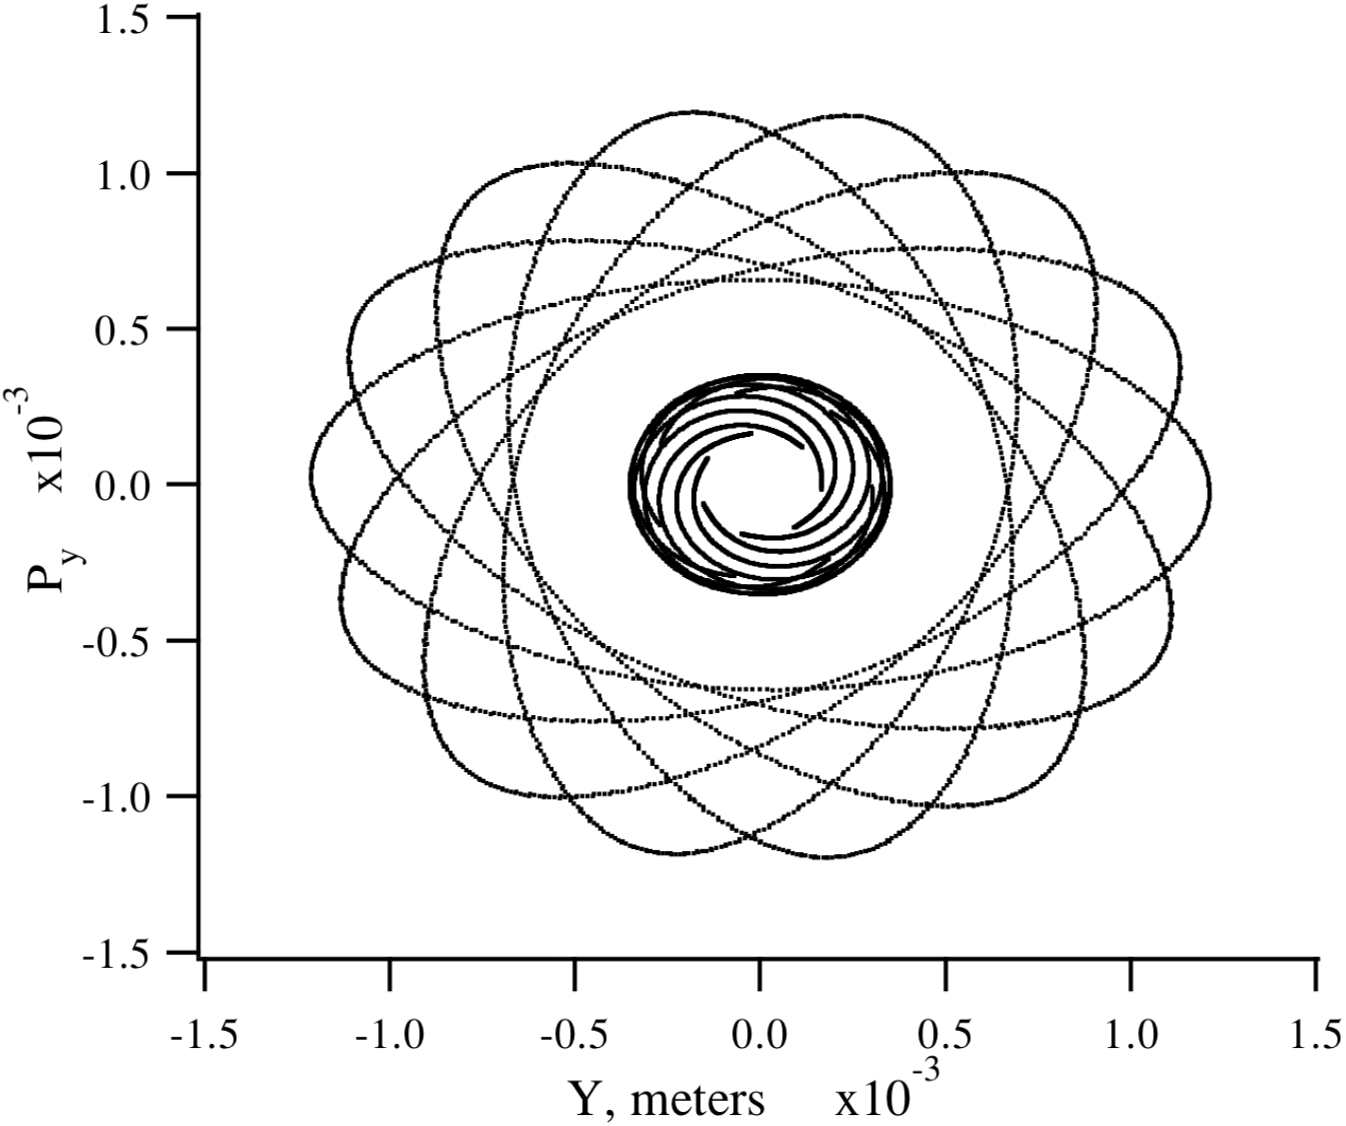
\includegraphics[scale=0.443]{sscy}
  \caption{Vertical phase-space projection for trajectories
       of two particles in a Superconducting Super Collider.
}
\end{figure}
